\documentclass[11pt,a4paper]{article}
% Packages every document in this directory shares. Kept apart from
% notation.tex so a symbol change and a package change are separate reviews.
\usepackage[margin=1in]{geometry}
\usepackage{amsmath}
\usepackage{amssymb}
\usepackage{booktabs}
\usepackage{graphicx}
\usepackage{tikz}
\usetikzlibrary{shapes.geometric}
\usepackage{microtype}
\usepackage{algorithm}
\usepackage{algpseudocode}
\usepackage[numbers]{natbib}
\usepackage[hidelinks]{hyperref}

% The one visual vocabulary the problem-statement sketches share. Circles are
% variables, squares are factors, shading marks where an observation enters,
% and a triangle marks a factor that gates on a second variable. Each of the
% eleven sketches carried a private copy, between them four circle diameters,
% three square sizes and four fonts, so a reader learned the convention once
% per figure (issue #529). A figure that needs a shape of its own adds it
% locally, on top of these.
\tikzset{
  fgvariable/.style={circle, draw, fill=white, minimum size=0.58cm,
                     inner sep=0.5pt, font=\footnotesize},
  fgobserved/.style={fgvariable, fill=black!12},
  fgfactor/.style={rectangle, draw, fill=white, minimum size=0.16cm,
                   inner sep=0pt},
  fgdata/.style={fgfactor, fill=black!25},
  fgindicator/.style={fgfactor, fill=black!55},
  fggate/.style={regular polygon, regular polygon sides=3, draw, fill=white,
                 minimum size=0.25cm, inner sep=0pt},
  fglink/.style={draw, thick},
  fgabsent/.style={draw, thin, gray, dashed},
  fgnote/.style={anchor=west, font=\footnotesize}
}

% Shared notation for every document in this directory.
%
% One definition per symbol, input by both the paper and the textbook, so a
% symbol cannot mean two things in two places (issue #249). A document that
% needs a symbol adds it here rather than defining its own; the notation table
% in the textbook is generated from this list by hand and reviewed against it.

% --- Structures ----------------------------------------------------------
\newcommand{\tree}{\mathcal{T}}          % a tree topology
\newcommand{\graph}{\mathcal{G}}         % a general undirected graph
\newcommand{\states}{\mathcal{A}}        % the state alphabet
\newcommand{\rootnode}{\rho}             % the root of a rooted tree
\newcommand{\neighbourhood}{\mathcal{N}} % a discrete move neighbourhood

% --- Continuous parameters ------------------------------------------------
\newcommand{\Q}{\mathbf{Q}}              % a rate matrix
\newcommand{\Pmat}{\mathbf{P}}           % a transition probability matrix
\newcommand{\SubMat}{\mathbf{S}}         % a symmetric exchangeability matrix
\newcommand{\bpi}{\boldsymbol{\pi}}      % a stationary or initial distribution
\newcommand{\branch}{\boldsymbol{\tau}}  % branch lengths
\newcommand{\params}{\boldsymbol{\theta}}% unconstrained parameters
\newcommand{\constrained}{\phi}          % the constraint map

% --- Data and objectives --------------------------------------------------
\newcommand{\data}{\mathbf{D}}           % observed data
\newcommand{\objective}{\mathcal{L}}     % the scalar being optimized
\newcommand{\energy}{H}                  % a Hamiltonian
\newcommand{\hidden}{\mathbf{Z}}         % a hidden state path
\newcommand{\emission}{\mathcal{E}}      % an emission family

% --- Reading a generated caption -----------------------------------------
% The captions under figures/ are written by the QA build, never by hand
% (docs/CLAUDE.md). This reads one in so a document quotes it rather than
% restating it.
\newread\qacaptionfile
\newcommand{\qacaptionread}[2]{%
  \begingroup
  \endlinechar=-1
  \openin\qacaptionfile=#1\relax
  \global\read\qacaptionfile to #2
  \closein\qacaptionfile
  \endgroup
}


\title{Graph-Structured Models, Their Algorithms, \\
and the Properties That Referee Them}
\author{M.\ J.\ Wilson}
\date{\today}

\begin{document}
\maketitle

\begin{abstract}
\noindent
A self-contained account of the problem classes this project supports---four
primary ones and the instances derived from them---the algorithms that solve
them, and---the part a methods section usually omits---the mathematical
properties each algorithm is validated against, and why those properties are
the right referees. Written for a reader with a scientific and
performance-computing background but none in phylogenetics or statistical
physics. It describes \emph{algorithms}, not an implementation: no result here
depends on how any of it is coded, and the companion paper carries the results.
\end{abstract}

\tableofcontents

\section{Notation}
\label{sec:notation}

One symbol, one meaning, across this document and the companion paper.

\begin{center}
\begin{tabular}{ll}
\toprule
Symbol & Meaning \\
\midrule
$\tree$        & a tree topology \\
$\graph$       & a general undirected graph \\
$\states$      & the state alphabet, $|\states| = k$ \\
$\rootnode$    & the root of a rooted tree \\
$\neighbourhood(\cdot)$ & the neighbourhood a discrete move set reaches in one step \\
$\Q$           & a rate matrix; $\Pmat(t) = \exp(\Q t)$ its transition matrix \\
$\SubMat$      & a symmetric exchangeability matrix \\
$\bpi$         & a stationary or initial distribution \\
$\branch$      & branch lengths \\
$\params$      & unconstrained parameters, $\params \in \mathbb{R}^d$ \\
$\constrained$ & the constraint map, $\constrained(\params)$ the feasible parameters \\
$\data$        & the observed data \\
$\objective$   & the scalar being minimized \\
$\energy$      & a Hamiltonian \\
$\hidden$      & a hidden state path \\
$\emission$    & an emission family \\
$\parity$      & a parity-check matrix; the codewords are the $c$ with $\parity c = 0$ \\
$\hadamard$    & the Sylvester--Hadamard matrix, italic where $\parity$ is bold \\
\midrule
$x_i$          & a discrete variable of a factor graph, $x_i \in \states$ \\
$\psi_a$       & a factor: a non-negative function of the variables $x_{\partial a}$ it touches \\
$m_{a \to i},\ m_{i \to a}$ & a message from factor to variable, and from variable to factor \\
$b_i,\ b_a$    & a belief: the marginal of a variable or a factor, exact on a tree \\
$Z$            & a partition function; $\log Z$ the evidence \\
$T,\ \beta = 1/T$ & a temperature and its inverse; a schedule is $T(t)$ over a budget of $t$ steps \\
\bottomrule
\end{tabular}
\end{center}

Two conventions are load-bearing later. Optimization is always
\emph{minimization}, so a likelihood-based objective is a negative
log-likelihood. And $\objective$ is a function of $\params$, the unconstrained
vector, not of the parameters a person names---the two are connected by
$\constrained$, and Section~\ref{sec:abstraction} says why the distinction is
not cosmetic.

A third governs the symbols the problem sections keep. Every model below is an
instance of the factor graph of Section~\ref{sec:factor-graph}, and its
variables are the $x_i$ of that section; but a spin is written $\sigma_i$ and a
hidden state $z_t$, the names a reader arrives with. The identification is made
once, where each model is stated as a factor graph: $x_i \equiv \sigma_i$ on a
Potts graph, $x_t \equiv z_t$ on a chain, $x_u \equiv z_u$ at a node of a tree.
Every section then carries the same five parts, in this order: the model; the
sizes it is supported at, from the fixtures and the size tiers; the model as a
factor graph, with a sketch of that structure; the algorithms as instances of
Equation~\ref{eq:sum-product} or of the optimization each is, stated in the
appendix and cited from the section; and the validation, one referee at a time
with what it does and does not establish. What differs between the problems is
then visible as content rather than presentation, and a section missing one of
the five parts fails a guard rather than a review.

\section{The Shape All Four Problems Share}
\label{sec:shape}

Each problem class below couples a \emph{combinatorial} search over a
structure to a \emph{continuous} optimization of parameters given that
structure. The two are not interleaved steps of one optimizer: a structural
move changes what the parameter vector \emph{means} and how long it is, so it
constructs a new objective rather than stepping inside an existing one.
Everything else here follows from that division.

\subsection{Factor Graphs: The One Structure}
\label{sec:factor-graph}

A tree under a substitution model, a Potts model on a graph and a hidden
Markov chain are one object: a set of discrete variables $x_1, \dots, x_N$ and
a set of factors $\psi_a$, each a non-negative function of a subset
$x_{\partial a}$, with
\begin{equation}
  p(x) = \frac{1}{Z} \prod_a \psi_a(x_{\partial a}),
  \qquad
  Z = \sum_x \prod_a \psi_a(x_{\partial a}).
  \label{eq:factor-graph}
\end{equation}
The bipartite graph between variables and factors is the factor graph
\citep{kschischang2001, koller2009}. In its \emph{normal} (Forney) form every
variable is an edge between exactly two factors, a variable shared by more
passing through an equality factor $\delta(x, x', \dots)$ \citep{forney2001};
the form changes the drawing and not the distribution, which is checked by
computing the same marginals on both. Observations enter as factors: a leaf's
state is an indicator, an emission a unary factor over the hidden state, so the
graph is over latent variables alone and a density and a probability are
handled alike.

Sum-product sends, from factor $a$ to variable $i$,
\begin{equation}
  m_{a \to i}(x_i) = \sum_{x_{\partial a \setminus i}}
    \psi_a(x_{\partial a}) \prod_{j \in \partial a \setminus i} m_{j \to a}(x_j),
  \qquad
  m_{i \to a}(x_i) = \prod_{b \in \partial i \setminus a} m_{b \to i}(x_i),
  \label{eq:sum-product}
\end{equation}
and on a tree one leaf-to-root and one root-to-leaf pass are exact
(Appendix~\ref{app:sum-product}): on the tree's factor graph this is pruning, Equation~\ref{eq:pruning}; on a chain it
is the forward recursion, Equation~\ref{eq:forward}; on a pairwise graph it
is Equation~\ref{eq:bp-message}. On a loopy graph the fixed point is the Bethe
approximation of Equation~\ref{eq:bethe}. Replacing the sum by a maximum gives
max-product, whose max-marginals carry the MAP assignment---on a chain,
Viterbi. One implementation of Equation~\ref{eq:sum-product} serves every
problem class, each pinned to the evaluator that predates it.

\paragraph{A coupled shape.}
The coupled spatio-sequential model puts a Potts prior on spatial labels
$\ell_n \in \{1..M\}$, one hidden chain $k_{s,m}$ per class, and a
\emph{gated} emission joining one label to one chain state:
\begin{equation}
  \log p(\ell, k, x) = \beta \sum_{\langle n,n' \rangle} J_{nn'}\,\delta(\ell_n, \ell_{n'})
    + \sum_m \Big[ \log \pi_m(k_{1,m}) + \sum_{s > 1} \log A_m(k_{s-1,m}, k_{s,m}) \Big]
    + \sum_n \sum_s \log P(x_{sn} \mid k_{s,\ell_n}, \theta_{\ell_n}) - \log Z_{\mathrm{Potts}},
  \label{eq:joint}
\end{equation}
Equation~\ref{eq:factor-graph} with pairwise, chain and degree-two gated
factors, and no fourth code path. Section~\ref{sec:coupled} states the model
in full, with the estimator its structure dictates.

\paragraph{A parity-check code.}
A low-density parity-check code is Equation~\ref{eq:factor-graph} with
binary variables, a unary factor per bit carrying the channel's
log-likelihood ratio, and a hard parity constraint per row of the check
matrix (Section~\ref{sec:ldpc}). It is the problem message passing was invented
for \citep{gallager1962}, and the fourth problem class: its decoder is
Equation~\ref{eq:sum-product} specialised to one number per message, held to
the general implementation on codes small enough for both.

\paragraph{What pins the general algorithm.}
Equation~\ref{eq:sum-product} is validated where each of its instances already
has an oracle, and by nothing new: on a tree-shaped Potts graph against
enumeration over $q^{|V|}$ configurations, on a chain against the sum over
$k^T$ paths, on a tree at one site against pruning, and on a loopy graph
against the pairwise belief propagation of Equation~\ref{eq:bp-message}---the
same approximation reached by two codes, which is agreement and not truth. The
Forney form is pinned by computing the same marginals on both drawings. An
algorithm agreeing only with itself is a second opinion, not an evaluator
(Section~\ref{sec:properties}).

\subsection{The Continuous Optimization Abstraction}
\label{sec:abstraction}

Let the objective be a differentiable scalar $\objective(\params)$ over an
unconstrained vector $\params \in \mathbb{R}^d$, with a map $\constrained$
carrying $\params$ to the constrained parameters a model is stated in:
positive branch lengths through a logarithm, a distribution over $k$ states
through a softmax on $k-1$ free values, a positive scale through a logarithm.

\paragraph{Why the map and not a projection.}
An optimizer that must be \emph{stopped} from leaving the feasible set will
eventually leave it, and a constrained parameter at its boundary has no
interval worth reporting. Constraining by construction removes both: every
point in $\mathbb{R}^d$ is feasible, and $\nabla_{\params} \objective$ is
defined everywhere.

\paragraph{Why the map must be injective.}
Where a reparameterization leaves $\objective$ unchanged, the direction along
it is not estimable: the observed information is singular and an interval
undefined. A softmax on $k$ free values has that flat direction---adding a
constant to every value changes nothing---which is why $k-1$ are used.
Removing the freedom is the constraint map's job, not the optimizer's.

\paragraph{What follows for inference.}
Standard errors come from the observed information at the optimum, pushed
through $\constrained$ by the delta method: $\mathrm{Var}(\constrained(\params))
\approx J \Sigma J^{\top}$ with $J$ the Jacobian of $\constrained$. An
\emph{asymptotic} statement, exact only in the large-sample limit, which is why
Section~\ref{sec:properties} makes realized interval coverage a measurement.

\subsection{Sampling the Posterior, and Adapting the Sampler}
\label{sec:hmc}

Where the delta-method interval is an approximation, the posterior can be
sampled instead and an interval read as a quantile. Hamiltonian Monte Carlo
\citep{neal2011} reads $\objective$ as a negative log density, adds a momentum
$p \sim \mathcal{N}(0, M)$, and proposes by integrating the Hamiltonian
$H(\params, p) = \objective(\params) + \tfrac{1}{2} p^{\top} M^{-1} p$ with a
symplectic integrator for $L$ steps of size $\varepsilon$, accepting with
probability $\alpha = \min\{1, \exp(-\Delta H)\}$. The integrator is reversible
and volume-preserving, so $\Delta H$ is the whole of the acceptance ratio, and
exact on the flow it conserves, so $\Delta H$ is bounded rather than growing
with $L$. A temperature enters as the momentum's variance, and a diagonal mass
$M = \mathrm{diag}(1/\sigma_i^2)$ as a change of coordinates,
$\phi_i = \params_i / \sigma_i$: the unit-mass dynamics on
$\objective(\sigma \odot \phi)$ are the mass-$M$ dynamics on $\params$ term for
term, so one integrator serves every metric and every temperature.

\paragraph{Adaptation, as a warm-up.}
The step $\varepsilon$ right for one posterior is wrong for the next, and the
coordinates' scales $\sigma_i$ are the posterior's. Both are set in a warm-up
whose draws are discarded, after which the chain runs at fixed values and has
the target as its stationary distribution; a chain that kept adapting would
not. The scales are the sample standard deviations of a warm-up window. The
step is driven to a target acceptance $\delta$ by dual averaging
\citep[Sec.~3.2]{hoffman2014}: after proposal $m$ with acceptance probability
$\alpha_m$,
\begin{equation}
  \bar h_m = \Big(1 - \frac{1}{m + t_0}\Big)\bar h_{m-1}
             + \frac{\delta - \alpha_m}{m + t_0}, \qquad
  \log \varepsilon_m = \mu - \frac{\sqrt{m}}{\gamma}\,\bar h_m, \qquad
  \log \bar\varepsilon_m = m^{-\kappa}\log \varepsilon_m
             + (1 - m^{-\kappa})\log \bar\varepsilon_{m-1},
  \label{eq:dual-averaging}
\end{equation}
with $\mu = \log(10\,\varepsilon_0)$ and the constants $\gamma$, $t_0$,
$\kappa$ setting the rate; the iterates $\varepsilon_m$ do not converge, the
averaged $\bar\varepsilon_m$ does, and the chain runs at the last of those. The
iteration runs twice, once at unit mass to estimate the scales and once on the
metric they define, since rescaling the coordinates changes the step right for
them.

\paragraph{Regime.}
On a target that is locally quadratic the leapfrog energy error is bounded
and oscillatory, so $\alpha(\varepsilon)$ stays near one up to the stability
limit $\varepsilon\,\omega_{\max} < 2$ on the stiffest direction and falls to
zero past it: a target of $\delta = 0.65$ lies \emph{on} that cliff, and an
iteration driven by a single Metropolis probability per proposal oscillates
across it and averages to a step whose acceptance is not $\delta$. Two
remedies, both measured rather than assumed: each proposal's step is drawn
uniformly from
$\bar\varepsilon\,(1 \pm j)$ \citep[Sec.~5.4.2.2]{neal2011}, which averages
$\alpha$ over the band and turns the cliff into a slope with one root; and
$\gamma$ is set larger than the value published for a trajectory-averaged
statistic, since the iterates' spread in $\log\varepsilon$ scales as
$1/(\gamma\sqrt{m})$. The chain after warm-up keeps the jitter, the step its
acceptance was adapted for, and every draw is still from a kernel with the
right stationary distribution.

\paragraph{A ladder from what it measures.}
The same principle sets a tempering ladder for Section~\ref{sec:tempering}. What
makes a ladder right is the exchange acceptance of Equation~\ref{eq:exchange}
between each neighbouring pair---near zero the replicas are independent chains,
near one a rung is redundant---so a warm-up measures it on a candidate ladder
and revises: a pair below a stated band is bisected at the geometric mean, a
rung both of whose pairs are above the band is removed, and a pair above the
band beside one inside it has their shared rung moved geometrically halfway
toward the far end of the pair inside. Geometric, because the exchange ratio
depends on the temperatures through $\beta_i - \beta_j$, so for an energy whose
spread the temperature sets, the acceptance is a function of the ratio of
neighbours. The endpoints are the caller's and never move; the warm-up's cost
in sweeps is charged to any comparison against a ladder set by hand.

\paragraph{What pins it.}
Equation~\ref{eq:dual-averaging} is arithmetic and is stepped by hand against
the implementation; the mass matrix is a change of coordinates and is held to
a mass-matrix leapfrog written out, to round-off. What a draw costs is the
effective sample size per gradient evaluation, with the size estimated by the
initial positive sequence \citep{geyer1992} and that estimator held to an
autoregressive chain whose integrated autocorrelation time is a closed form.
Three statistics follow: the adapted chain's acceptance lands within a stated
distance of $\delta$ over independent seeds; its posterior means and spreads
agree with a fixed-parameter chain's within Monte Carlo error, on the analytic
Gaussian and on a four-taxon tree; and the adapted ladder's exchanges lie
inside the band on the frustrated lattice, with its ground-state hit rate at
equal sweeps reported beside the hand ladder's. The fixed-parameter samplers
are unchanged and remain the oracles.

\subsection{The Discrete Search as a Decision Process}
\label{sec:policy-gradient}

The structural search is a Markov decision process \citep{suttonbarto2018}:
the state is the current structure with its fitted parameters, an action is a
move from the neighbourhood $\neighbourhood(\cdot)$, and the reward is the
improvement in the objective. An episode ends on a step budget or when no move
improves the score---a property of the state, and the stopping rule the greedy
baseline obeys, which is what makes the two comparable. The reward being a
difference, the undiscounted return telescopes,
\begin{equation}
  G = \sum_{t=0}^{T-1} R_t
    = \sum_{t=0}^{T-1} \big[\objective(s_t) - \objective(s_{t+1})\big]
    = \objective(s_0) - \objective(s_T),
  \label{eq:return}
\end{equation}
the improvement between the first and last state whatever path joined them.
That licenses an undiscounted return---a discount would prefer improvement
found early over the same improvement found late---and it is why a truncation
landing between a sacrifice and its payoff teaches the opposite of the truth,
so a truncated episode is recorded as one.

The policy is a softmax over the scores of the \emph{available} actions,
$\pi(a \mid s) \propto \exp f(s, a)$ for $a \in \neighbourhood(s)$, so a
neighbourhood of any size is admissible. A scorer with a single weight on the
improvement a move buys is an inverse temperature, and greedy search is its
zero-temperature limit; such an agent can learn only how much to accept a
worsening move to reach a better optimum, which is the credit-assignment
question this search makes sharp. That class cannot rank two moves differently
from hill climbing, so the tree environment also scores a move by what it
computes without a fit: the change in parsimony score, the fraction of sites
compatible with the split the move breaks and with the split it makes, and the
sizes of the two subtrees it exchanges, each standardized within the
neighbourhood. A feature constant over a neighbourhood is cancelled by the
softmax and excluded; the Robinson--Foulds distance from the current tree, the
same for every NNI neighbour, is the standing example. Whether the wider class
learns more is measured at a matched budget, never inferred from its width.
The policy is trained by the score-function estimator with a baseline,
\begin{equation}
  \nabla J = \mathbb{E}\Big[\sum_{t} \nabla \log \pi(a_t \mid s_t)\,
             \big(G_t - b(s_t)\big)\Big],
  \qquad G_t = \sum_{u \ge t} R_u,
  \label{eq:reinforce}
\end{equation}
where a baseline $b$ independent of the sample it is subtracted from leaves the
estimator unbiased and reduces its variance, not its bias: $G_t$ is a sum of
objective differences whose scale is the problem's, so an uncentred gradient
varies by orders of magnitude between instances. The comparison against the
greedy baseline is at a matched budget of objective evaluations per decision,
never in wall-clock time.

\paragraph{The scorer, and what is identifiable in it.}
The score $f(s, a)$ is a function of the action's features, and two
parameterizations serve. A \emph{linear} scorer, $f = w^{\top} x(s, a)$, is the
reference, because its weights are what a recovery test can state a truth
against: on the lattice environment the improvement a move buys decomposes
exactly into two features, so the greedy searcher \emph{is} a particular $w$
inside the policy class, and ``did the agent learn the landscape'' becomes a
statement about $w$ rather than about a loss curve. A
\emph{multilayer-perceptron} scorer --- two hidden layers over the same
features, one output per action --- is for a reward not linear in them. It is
measured against the linear one at a matched budget and never assumed better:
a wider class that is not needed costs sample efficiency and gives up the
recovery statement. Both share the softmax's gauge. Adding a constant to every
score in a state changes nothing, so a feature constant over the neighbourhood
carries no identifiable weight and is excluded, and neither scorer has a bias
term. The critic of Section~\ref{sec:actor-critic} shows the rule is about the
softmax and not about features: a value is not a softmax, a constant there
\emph{is} identifiable, and the critic carries one.

\paragraph{Exploration is declared, not learned.}
A softmax over improvements ends its episode at the first state no move
improves, so an agent chooses which local optimum to enter and can never
leave one. The remedy is to collect episodes under a \emph{behaviour} policy
that takes the trained policy's best action except with probability
$\epsilon$, where it draws uniformly from the neighbourhood --- the only way a
\emph{worsening} move is taken. It is not trainable and exposes no weights, so
a measured escape rate is attributable to $\epsilon$ and not to a training run
alongside it; $\epsilon$ follows a declared schedule over the iterations, as a
temperature does in Section~\ref{sec:tempering}. At $\epsilon = 0$ the agent
still walks, deterministically: past a local optimum the best available action
is the least-bad move, not the same object as a climb that would have stopped.

Two consequences for the accounting, both easy to get wrong in the direction
that flatters the agent. An episode allowed to continue past a local optimum is
scored on the \emph{best} state it saw and not its last, or a better searcher
looks worse the longer it runs. And the matched baseline is then greedy
\emph{with restarts}: a single greedy run stops after a few decisions and
leaves the rest of the budget unspent, so a result stated against it overstates
itself. One failure produces plausible numbers rather than an error ---
wrapping an \emph{untrained} policy is not hill climbing, since with equal
scores the best action is whichever the neighbourhood lists first, and what is
measured is exploration around a fixed arbitrary move.

\paragraph{What pins it.}
Equation~\ref{eq:return} is an identity and is asserted exactly on every
recorded episode. Equation~\ref{eq:reinforce} is an expectation, so its
estimator is pinned against the gradient of the exact expected return,
computable by enumerating every episode on a small environment, and the
baseline's unbiasedness by the same enumeration: the expected gradient with and
without $b$ agree. An environment small enough to enumerate is the oracle for
the learning machinery, as a tree small enough to enumerate is for the search.

\subsection{Actor--Critic and Proximal Policy Optimization}
\label{sec:actor-critic}
The baseline in \eqref{eq:reinforce} may depend on the state. The natural
choice is the state value $V^\pi(s) = \mathbb{E}[G_t \mid s_t = s]$, the
improvement the search still expects from $s$, estimated by a \emph{critic}
fitted to sampled returns; the estimator is then weighted by the
\emph{advantage} $A_t = G_t - V(s_t)$, unbiased for any critic and of least
variance in this family when the critic is exact (Appendix~\ref{app:rl}).
Where the return is exact by enumeration, so is $V^\pi$, and a critic is
scored against it rather than against its own loss. The Monte Carlo return and
the one-step bootstrap $R_t + V(s_{t+1})$ are the two ends of the
\emph{generalized advantage} \citep{schulman2016}, at $\gamma = 1$,
\begin{equation}
  A_t^{(\lambda)} = \sum_{l \ge 0} \lambda^l \delta_{t+l},
  \qquad
  \delta_t = R_t + V(s_{t+1}) - V(s_t),
  \label{eq:gae}
\end{equation}
with $V(s_T) = 0$ at a terminal state and the critic's value at a truncated
one; $\lambda = 1$ recovers $G_t - V(s_t)$ and $\lambda = 0$ the temporal
difference, trading the critic's bias against the return's variance.

The score-function estimator is valid only for the policy that collected the
episodes. \emph{Proximal policy optimization} \citep{schulman2017} reuses a
batch for several gradient steps by importance-weighting each decision with
$\rho_t = \pi(a_t \mid s_t) / \pi_{\mathrm{old}}(a_t \mid s_t)$ and clipping
the ratio's effect on the objective,
\begin{equation}
  \objective_{\mathrm{PPO}} = \mathbb{E}\Big[\sum_t
    \min\big(\rho_t A_t,\; \mathrm{clip}(\rho_t, 1-\epsilon, 1+\epsilon)\, A_t\big)\Big],
  \label{eq:ppo-clip}
\end{equation}
so an update cannot move the policy far from the one the advantages were
estimated under. At the collecting policy every ratio is one and, without
clipping, the gradient of \eqref{eq:ppo-clip} is the actor--critic's; the
regression suite pins that identity and measures on the Potts chain what the
reuse buys: the fraction of the 81 starts from which the trained policy reaches
the enumerated optimum, at a matched number of episodes. The same ratio makes
the update valid when a \emph{behaviour} policy collected the episodes: with
$\pi_{\mathrm{old}}$ replaced by $\beta$, the $\epsilon$-greedy wrapper of the
policy being trained, the search can leave a local optimum the softmax would
settle into, and the estimator is corrected by $\pi / \beta$.

\paragraph{What the critic reads, and what it may not.}
$V$ is a function of the state, while the decision process supplies features
of \emph{actions}. The state's features are therefore aggregates over its
neighbourhood --- the mean and the maximum of the action features, and the
logarithm of the neighbourhood's size --- covering every instance without
widening the interface, a terminal state having no actions and so the zero
vector. Appendix~\ref{app:rl} carries the rule that makes the baseline
legitimate: the critic may read the state and never the action sampled at that
step. Where the return is exact by enumeration $V^\pi$ is exact too, and the
critic is scored against \emph{that}; a critic scored against its own training
loss can fit its targets, miss $V^\pi$, and leave an estimator unbiased and
useless.

\paragraph{Off-policy, and what the ratio costs.}
Equation~\ref{eq:ppo-clip} is one case of a general correction. For any
behaviour policy $\beta$ with $\beta(a \mid s) > 0$ wherever $\pi(a \mid s) >
0$, weighting each decision by $\rho_t = \pi(a_t \mid s_t) / \beta(a_t \mid
s_t)$ makes the estimator of Equation~\ref{eq:reinforce} unbiased for $\pi$ on
episodes that $\beta$ collected \citep{suttonbarto2018}. The support condition
is not a technicality: an action $\beta$ never samples contributes nothing, so
a \emph{deterministic} behaviour policy corrects nothing. That is the second
reason for the exploring wrapper's uniform draw, and why its mixture must be
available as a distribution and not only as a sampler --- $(1 - \epsilon)$ on
the best action and $\epsilon / |\neighbourhood(s)|$ everywhere is what the
ratio divides by. That $\epsilon$ is the exploration rate; the one in
Equation~\ref{eq:ppo-clip} is a clip width, and the two are unrelated.

The correction costs variance, and the cost has a shape. A ratio is unbounded
above, so one decision the behaviour policy made rarely can dominate a batch;
a weight formed as the \emph{product} of ratios along a trajectory is worse,
its variance growing with the episode length. Two answers are carried, and
they are not the same. The per-decision form of Equation~\ref{eq:ppo-clip}
weights each step by its own ratio rather than the trajectory's product, which
removes the growth with episode length. The clip bounds the ratio's effect on
the objective, and so the size of an update, while leaving the estimator's
variance where it was: a trust region and not a variance reduction, and
reading it as the second is the standing error about it.

\subsection{Planning with a Learned Prior and Value}
\label{sec:planning}
A policy answers ``which move'' from what it has seen; a planner looks
ahead. From the current state, each of $n$ simulations descends a tree of
successors choosing, at every expanded node, the child that maximizes
\begin{equation}
  Q(s, a) + c\, \pi(a \mid s)\, \frac{\sqrt{N(s)}}{1 + N(s, a)},
  \label{eq:puct}
\end{equation}
the mean return backed up through that child plus an exploration bonus that
is the prior the policy gives the move, decaying with the child's visits
\citep{silver2017}; the first unexpanded child is scored by the critic and the
return backed up to the root. The root's visit counts, normalized, are a
policy that improves on the prior, and \emph{expert iteration}
\citep{anthony2017} trains the policy toward that distribution by cross-entropy
and the critic toward the achieved return, so the planner's answers become the
policy's. Every expansion evaluates a successor, so the search is counted in
the unit the rest of this document counts, and the comparison with greedy
states the rate and the evaluations together (Appendix~\ref{app:rl}).

\paragraph{Compound moves.}
A move set fixes the granularity of a decision, and a search whose
neighbourhood holds one interchange must find a sacrifice and its payoff as two
decisions --- the credit assignment a truncated episode destroys. An
\emph{option} is a policy over primitive moves with an initiation set and a
termination rule, so a sequence that pays off only as a unit becomes one
decision and is credited as one \citep{sutton1999}; the termination rule can be
learned beside the policy that calls it \citep{bacon2017}. Nothing here builds
one, and the budget rule says what it would have to survive: a compound move
evaluates every primitive it composes, so an option reaching a better optimum
by evaluating more candidates than hill climbing has not won.

\paragraph{Planning with a learned model.}
The planner above expands the \emph{true} successor and reads the true reward,
affordable only because a move's reward is a closed form at known parameters.
It stops being affordable the moment the reward is a fit per candidate, the
regime every problem here is in. The answer is then to plan on a learned model:
a transition and a reward in a latent space, trained so that the values,
policies and rewards the plan reads agree with the observed ones, and not so
that the latent state reconstructs the real one \citep{schrittwieser2020}.
Requiring only the quantities the search reads to be right makes it a method
rather than a reconstruction, and makes it checkable here: on an instance small
enough to enumerate, a planner on a learned model must return an optimal action
wherever the planner on the true one does. It is not built.

\subsection{Relaxing a Discrete Decision}
\label{sec:relaxation}
A third route past a discrete search is to make it continuous. Write a
configuration over $L$ sites and $k$ states as a row-stochastic $q$, one
simplex per site, and read the discrete score on it. Two demands separate a
relaxation from a second model, and both are checkable.

\emph{It must be an extension of what it relaxes.} At every vertex --- every
one-hot $q$ --- the relaxed value must equal the discrete score exactly,
asserted over every configuration of an enumerable instance. A relaxation
merely close at the corners optimizes a different problem and nothing measured
on it transfers --- the demand Section~\ref{sec:tropical} makes of the tropical
relaxation, and the reason Equation~\ref{eq:tropical-corner} is a derived
tolerance rather than a constant.

\emph{Its boundary is multilinearity, not the shape of the graph.} If every
term of the score involves at most one factor from each site, then under a
factorized $q$ distinct sites are independent and each term's expectation is
that term at the marginals:
\begin{equation}
  \mathbb{E}_{q}\big[\,\mathrm{score}(x)\,\big] = \mathrm{score}(q),
  \label{eq:multilinear}
\end{equation}
exactly, so the form evaluated at the marginals \emph{is} the expected discrete
score and not an approximation. The condition is easy to state wrongly. It is
not that the model must be a chain --- a lattice is as multilinear --- nor that
the terms must be pairwise, a term coupling three \emph{distinct} sites being
one factor per site. What breaks it is a term reading one site twice, since for
an indicator $\mathbb{E}[X^2] = \mathbb{E}[X] \neq \mathbb{E}[X]^2$. Two things
follow. A multilinear function on a product of simplices attains its maximum at
a vertex, so the relaxation introduces no optimum the discrete problem lacks
and what a relaxed search loses is lost to the ascent. And the deterministic
relaxation needs no sampling, which sharpens the question about the stochastic
one: since Equation~\ref{eq:multilinear} is exact, whatever bias an estimator
shows belongs to the estimator.

Sampling a relaxed configuration is the Gumbel-softmax: perturb each site's
log-probabilities by independent Gumbel noise and take a softmax at
temperature $\tau$ where an $\arg\max$ would give a draw, which is
reparameterized --- differentiable in the probabilities --- and biased at every
$\tau > 0$, exact only in a limit where the gradient vanishes. The bias is
measured against the exact gradient enumeration supplies and never assumed
small, and the score-function estimator of Equation~\ref{eq:reinforce} is the
unbiased alternative at higher variance: Section~\ref{sec:actor-critic}'s trade
in a second place. Carrying the construction from one categorical variable to a
\emph{structured} object, where the $\arg\max$ is a combinatorial solver rather
than a coordinate, is the stochastic-softmax-trick family \citep{paulus2020}
--- what a differentiable topology would need, and the direction
Section~\ref{sec:tropical} approaches from the other side.

\subsection{Surrogates and Bounds}
\label{sec:surrogates}
The evaluation a discrete search pays for---a fit of $\branch$ per topology,
or $\log Z$ for a lattice---is what makes the search expensive, so each
problem carries \emph{surrogates}: cheaper functions of the structure standing
in for it. A surrogate makes a claim --- a lower bound, an upper bound, or a
point prediction --- and the claim is part of the object. An analytic bound is
proved (Appendix~\ref{app:bounds}) and \emph{certified}: checked against the
exact value on every structure an oracle can score, with no violation allowed.
A learned predictor is \emph{calibrated} instead, shifted by a quantile of its
held-out residuals, and certified to the coverage it claims. The search ranks a
neighbourhood by a surrogate and fits only the top candidates
(Algorithm~\ref{alg:surrogate-rank}); the accepted move is always evaluated in
full, so a surrogate changes what is fitted and never what is reported.

For a topology the maximized log-likelihood $\ell^\ast(\tree) = \max_{\branch}
\ell(\tree, \branch)$ is bracketed by two one-pass quantities. Any feasible
lengths give a lower bound, and lengths $\hat{\branch}$ solved by
non-negative least squares from the pairwise Jukes--Cantor distances
$\hat d_{ab}$ are feasible:
\begin{equation}
  \ell(\tree, \hat{\branch}) \;\le\; \ell^\ast(\tree),
  \qquad
  \hat{\branch} = \arg\min_{\branch \ge 0}
    \sum_{a<b} \Big(\sum_{e \in \mathrm{path}(a,b)} \tau_e - \hat d_{ab}\Big)^2 .
  \label{eq:plugin-bound}
\end{equation}
Under Jukes--Cantor $\Pmat(t) = a\,\mathbf{I} + (1-a)\,\mathbf{J}/k$ with
$a = e^{-kt/(k-1)}$, so a site likelihood is multilinear in the $a_e$ and its
maximum over the box $[0,1]^{|E|}$ sits at a vertex, where every branch
either forbids a change or forgets the parent's state at cost $1/k$. With the
tree rooted at the first leaf, the vertex maximum of site $s$ is
$\pi(x_{1,s})\,k^{-F_s(\tree)}$ for the site's Fitch score $F_s$, whence
\begin{equation}
  \ell^\ast(\tree) \;\le\; \sum_s \log \pi(x_{1,s}) \;-\; F(\tree)\,\log k .
  \label{eq:parsimony-bound}
\end{equation}
Both apply to a subtree as they do to the tree.

A third trades exactness for cost by the site count rather than the tree.
Site-pattern compression, Equation~\ref{eq:site-patterns}, is exact and
saturates; blocks of $N > 1$ consecutive sites repeat too rarely for the same
identity to save anything, so a block partition buys a bracket instead.
Partition the $L$ columns into $\lceil L/N \rceil$ blocks of $N$
consecutive sites, and let $\mathcal{F}$ be the blocks occurring at least $m$
times. Evaluate those exactly, by Equation~\ref{eq:site-patterns} over their
columns, and bound the remaining $B$ sites by the extremes of a single site's
log-likelihood over the whole column alphabet
(Algorithm~\ref{alg:block-frequency}):
\begin{equation}
  \ell_{\mathcal{F}} + B \, \underline{\lambda}(\tree, \branch)
  \;\le\; \ell(\tree, \branch) \;\le\;
  \ell_{\mathcal{F}} + B \, \overline{\lambda}(\tree, \branch),
  \qquad
  \begin{aligned}
    \underline{\lambda} &= \textstyle\min_{x \in \states^n}
      \log p(x \mid \tree, \branch, \Q), \\
    \overline{\lambda} &= \textstyle\max_{x \in \states^n}
      \log p(x \mid \tree, \branch, \Q),
  \end{aligned}
  \label{eq:block-frequency-bound}
\end{equation}
with $\ell_{\mathcal{F}}$ the frequent blocks' own log-likelihood. Both
$\underline\lambda$ and $\overline\lambda$ are had in one pass over the tree
and independently of $L$, by Equation~\ref{eq:pruning} with each leaf's
message replaced by the extremes of its transition row
(Appendix~\ref{app:bounds}); relaxing them to those one-pass values makes the
bracket cheap and makes it loose. The width is exactly
$B\,(\overline\lambda - \underline\lambda)$, so the cutoff $m$ sets the trade:
$m = 1$ leaves $B = 0$ and returns the exact value, and raising $m$ moves
blocks into the tail and never out. Only the lower end bounds
$\ell^\ast(\tree)$, by the argument Equation~\ref{eq:plugin-bound} rests on.
Measured at five taxa and 2,000
sites, $N = 1$ and $m = 8$ leaves a width of $1.0\,|\ell|$ and $N \ge 3$
leaves the whole alignment in the tail, so neither end orders topologies and
what ranks is $\ell_{\mathcal{F}}$ itself, a point prediction over a fixed
subsample that claims nothing.

For a lattice the partition function is bracketed by two variational
quantities. The naive mean-field bound is Gibbs' inequality at a product
distribution $q = \prod_i q_i$, tightest at its fixed point:
\begin{equation}
  \log Z \;\ge\; \sum_i \sum_\sigma q_i(\sigma)\, h_i(\sigma)
    + \sum_{\langle i,j \rangle} J_{ij} \sum_\sigma q_i(\sigma)\, q_j(\sigma)
    - \sum_i \sum_\sigma q_i(\sigma) \log q_i(\sigma) .
  \label{eq:mean-field-bound}
\end{equation}
Because $\log Z$ is convex in the parameters, Jensen's inequality over a
distribution $\rho$ on spanning trees $T$, with parameters $\theta(T)$
supported on $T$ and averaging to $\theta$, gives an upper bound each term of
which is exact by one leaf-to-root pass:
\begin{equation}
  \log Z(\theta) \;\le\; \sum_T \rho(T)\, \log Z\big(\theta(T)\big),
  \qquad
  \sum_T \rho(T)\,\theta(T) = \theta ,
  \label{eq:spanning-tree-bound}
\end{equation}
the tree-reweighted bound of \citet{wainwright2005}. From any bracket
$L \le \log Z(\beta) \le U$ at inverse temperature $\beta$, and
$e^{-\beta E_{\min}} \le Z(\beta) \le k^N e^{-\beta E_{\min}}$,
\begin{equation}
  -\frac{U}{\beta} \;\le\; E_{\min} \;\le\; \frac{N \log k - L}{\beta} .
  \label{eq:ground-state-bounds}
\end{equation}

\subsection{Reading a Comparison}
\label{sec:comparisons}
Every problem statement below ends with the same question: given more than one
method that applies, which is worth a budget at the sizes that section
supports. Three axes answer it, asked in the same order.

\emph{The precondition} is a structural property of the instance deciding
whether a method may run at all, and it is not a matter of degree: a
non-negative coupling, a metric on labels, a tree, a terminated trellis, an
output-symmetric channel. A method whose precondition fails is refused rather
than run badly, which separates the comparisons here from a ranking --- a cell
of Section~\ref{sec:applicability} is empty where a precondition failed as
often as where nobody wrote the code.

\emph{The cost} is counted in the unit that problem counts: objective
evaluations for a discrete search, sweeps for a sampler, passes over the
graph for a marginalization, configurations for an enumeration. It is never
counted in seconds. A cost in operations and in the live set a recursion holds
is a property of the algorithm and transfers between machines; a wall clock is
a property of neither, and the language a kernel is expressed in --- and the
boundary between it and the language that calls it --- measures a small
fraction of a call rather than the term that decides a method. No choice here
turns on it, and the measurements belong to the companion paper.

\emph{The reach of the referee} is the size past which nothing exact scores the
answer. It changes what may be \emph{claimed} rather than what may be run:
inside it a method is scored against a truth, outside it against a recovered
structure, a bound, or another method --- agreement and not truth
(Section~\ref{sec:properties}). Two methods that agree inside the reach and
diverge outside it have not been separated, and a comparison crossing the reach
without saying so has changed its subject mid-sentence.

Where the three leave a genuine choice, the answer is a measurement at an equal
budget in the problem's own unit over shared seeds, and a statement about that
instance. Where they do not, the section says which of the three decided.

\paragraph{What a referee assumes about the application.}
A referee is only as good as the property it rests on, and those properties are
not shared: each is a fact about the model its section states and would be
false of a neighbouring one. Table~\ref{tab:referee-assumptions} collects them,
one per problem, so a result read out of one section carries the assumption it
was refereed under.

\begin{table}[htbp]
  \centering
  \footnotesize
  \begin{tabular}{@{}p{0.19\textwidth}p{0.38\textwidth}p{0.37\textwidth}@{}}
    \toprule
    Problem & The property its referees rest on & What is unrefereed without it \\
    \midrule
    Phylogenetic inference (\ref{sec:phylo})
      & Sites are independent and identically distributed given the tree,
        and the model is time-reversible.
      & Pattern compression stops being an identity, and the pulley
        principle stops holding, so the root's position becomes an
        estimand rather than a gauge. \\
    Potts models (\ref{sec:potts})
      & The move set reaches every configuration the enumeration sums over,
        and the number of moves in a sweep does not depend on the state.
      & The goodness-of-fit test reports a chain that has not mixed as a
        chain drawing from the wrong distribution, and the two failures are
        indistinguishable in its output. \\
    Hidden Markov models (\ref{sec:hmm})
      & The emission family's declared support, and identifiability up to
        the permutation of hidden states.
      & A bound written for a probability is asserted of a density, and
        recovery compares two parameter sets under different labellings. \\
    Coupled model (\ref{sec:coupled})
      & The gated factor has degree two, so a per-class posterior is a
        chain posterior.
      & The expectation step is an approximation of the posterior rather
        than the posterior, and the enumerated instance referees the wrong
        quantity. \\
    Large parsimony (\ref{sec:parsimony})
      & The step matrix is a metric, so every rooting of an unrooted
        topology scores the same.
      & The score depends on a rooting the search does not carry, and the
        enumeration referees a different criterion at each. \\
    Frustrated lattices (\ref{sec:frustrated})
      & The periodic geometry the counting argument closes on, and that a
        planted state is an upper bound and not the optimum.
      & An energy asserted at every size is asserted of a lattice the count
        does not close on, and a search reaching the planted energy is read
        as having succeeded. \\
    Gaussian mixture (\ref{sec:mixture})
      & Observations are independent, and the components separate enough
        that an ordering resolves the permutation.
      & The alignment matches the wrong component, and a failure of the
        labelling is reported as a failure of the fit. \\
    Count-emission mixture (\ref{sec:emissionmixture})
      & The posterior factorizes across observations, and the trial count's
        form is declared.
      & The enumeration over a prefix says nothing about the remaining
        observations, which is the whole of what it is for. \\
    Test functions (\ref{sec:testfunctions})
      & The published minimizers, and that the surface is not a likelihood.
      & Nothing: this is the one problem whose referee costs nothing at any
        size, which is why it is carried. \\
    Parity-check decoding (\ref{sec:ldpc})
      & Channel output symmetry, and a declared stopping rule that counts a
        capped iteration as a failure.
      & Every rate measured past the encoder's reach is a rate on one word
        rather than on the code. \\
    Turbo decoding (\ref{sec:turbo})
      & Both trellises terminated, and the same output symmetry carried
        through a recursive encoder and the message map.
      & The recursion's boundary is an assumption rather than a fact, and
        one constituent decoder stops being exact. \\
    \bottomrule
  \end{tabular}
  \caption{The application-specific property each problem's validation rests
  on, and what stops being refereed where it fails. The properties are not
  interchangeable and none is inherited: each is a fact about the model its
  own section states.}
  \label{tab:referee-assumptions}
\end{table}

\section{Problem Statement: Phylogenetic Inference}
\label{sec:phylo}

\subsection{The model}
\label{sec:phylo:model}
Character evolution along a branch is a continuous-time Markov chain with rate
matrix $\Q$; the transition probabilities over a branch of length $t$ are the
matrix exponential $\Pmat(t) = \exp(\Q t)$ \citep{felsenstein2004}. A
time-reversible model factors as $\Q = \SubMat \operatorname{diag}(\bpi)$ with
$\SubMat$ symmetric, and then satisfies detailed balance,
$\pi_i \Q_{ij} = \pi_j \Q_{ji}$.

The simplest such model is Jukes--Cantor on $k$ states: every substitution
equally likely and $\bpi$ uniform, with $\Q$ scaled so that one unit of branch
length is one expected substitution per site,
\begin{equation}
  -\sum_{i \in \states} \pi_i\, \Q_{ii} = 1,
  \label{eq:normalization}
\end{equation}
which puts the transition probabilities in closed form
\citep{felsenstein2004, durbin1998}:
\begin{equation}
  \Pmat_{ij}(t) = \frac{1}{k} + \Big(\delta_{ij} - \frac{1}{k}\Big)\,
                  \exp\!\Big(-\frac{k}{k-1}\, t\Big).
  \label{eq:jc}
\end{equation}
Rows sum to one, $\Pmat(0) = \mathbf{I}$, and every entry tends to $1/k$ as
$t \to \infty$; the general time-reversible model replaces the single rate by
$\SubMat$ and $\bpi$, keeping Equation~\ref{eq:normalization}.

Given a topology $\tree$ over $n$ taxa, branch lengths $\branch$, and an
alignment $\data$ of $L$ sites, sites evolve independently and the likelihood
marginalizes every assignment $z$ of states to the internal nodes:
\begin{equation}
  p(\data \mid \tree, \branch, \Q)
    = \prod_{s=1}^{L} \;\sum_{z}\; \pi_{z_{\rootnode}}
      \prod_{(u \to v)} \Pmat_{z_u z_v}(\tau_v),
  \label{eq:site-independence}
\end{equation}
the product over the branches $(u \to v)$ of the rooted tree with the leaves
fixed by the data---$k^{\,n-2}$ terms per site for a binary tree. Summing it
directly is the oracle every faster evaluation is checked against.

\paragraph{Supported sizes.}
\label{par:phylo:sizes}
The declared range is $n \in [10, 1000]$ taxa by $L \in [100, 11{,}000]$ sites,
and the largest evaluation measured is 200 taxa by 11,000 sites. What is
\emph{refereed} is smaller, the referee being an enumeration: the $(2n-5)!!$
unrooted topologies number 15 at five taxa, 105 at six, 945 at seven and 10,395
at eight, so the per-pull-request tier carries the five- and six-taxon
fixtures, the stress tier seven, and the release tier eight and the twenty- and
fifty-taxon trees that only the distance start referees. Direct
marginalization over the $k^{\,n-2}$ internal assignments of
Equation~\ref{eq:site-independence} referees the likelihood on the same
fixtures at $k = 4$ and $L$ from 200 to 200,000 sites. The Hadamard start is
offered from three to twelve taxa, its spectrum having $2^{n-1}$ entries, and
every enumeration here refuses more than 200,000 configurations rather than
attempting them.

\subsection{As a factor graph}
One site is one instance of Equation~\ref{eq:factor-graph}. The variables are
the states $x_u \equiv z_u \in \states$ at every node $u$ of the rooted tree,
leaves included. The factors are the root prior $\psi_{\rootnode}(x_{\rootnode})
= \pi_{x_{\rootnode}}$, one pairwise factor per branch,
$\psi_v(x_u, x_v) = \Pmat_{x_u x_v}(\tau_v)$ for $u$ the parent of $v$, and one
indicator per leaf, $\psi_\ell(x_\ell) = \mathbb{1}[x_\ell = \text{observed}]$,
which folds the data in. The bipartite graph is a tree, so
Equation~\ref{eq:sum-product} is exact, and $Z$ is the site likelihood
$p(\data_s \mid \tree, \branch, \Q)$; sites being independent
(Equation~\ref{eq:site-independence}), the alignment's likelihood is the
product of $L$ such $Z$. In the Forney form every internal node's state is an
edge through an equality factor of degree three---two branches and, at the
root, the prior---which is the drawing Section~\ref{sec:coupled} uses.
Figure~\ref{fig:phylo:sketch} is that structure on four taxa.

% The tree factor graph of Section~\ref{sec:phylo}, drawn by hand on the eight
% taxa of the release fixture. Input by textbook.tex; a sketch and not a
% rendered figure, so it is outside the figure cache and the render cap, which
% govern generated output only. The branch lengths are those of
% tests/regression/fixtures/tree_jc/release.yaml, and the horizontal axis is
% their unit: one node's depth is the sum of the lengths above it.
\begin{figure}[htbp]
\centering
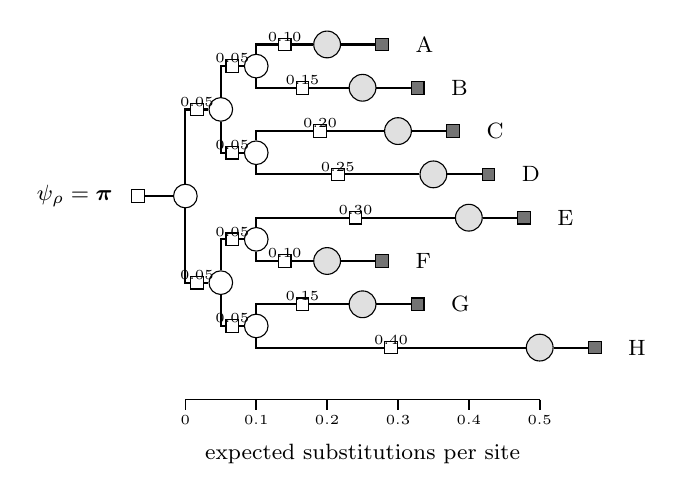
\begin{tikzpicture}[
    x=9cm, y=0.55cm,
    fgsmall/.style={fgvariable, minimum size=0.30cm, inner sep=0pt},
    blen/.style={font=\tiny, inner sep=1pt},
    taxon/.style={anchor=west, font=\footnotesize}
  ]
  % node name/depth/height
  \foreach \n/\d/\h in {%
      root/0/3.5, l/0.05/5.5, ll/0.10/6.5, lr/0.10/4.5,
      r/0.05/1.5, rl/0.10/2.5, rr/0.10/0.5}
    { \node[fgsmall] (\n) at (\d, \h) {}; }
  \foreach \n/\d/\h/\t in {%
      A/0.20/7/A, B/0.25/6/B, C/0.30/5/C, D/0.35/4/D,
      E/0.40/3/E, F/0.20/2/F, G/0.25/1/G, H/0.50/0/H}
    { \node[fgobserved, minimum size=0.34cm, inner sep=0pt] (\n) at (\d, \h) {};
      \node[fgfactor, fill=black!55] (i\n) at (\d, \h) [xshift=7mm] {};
      \draw[fglink] (\n) -- (i\n);
      \node[taxon] at (\d, \h) [xshift=10mm] {\t}; }
  % parent/child/length: a square branch, the factor at the midpoint of its
  % horizontal segment, the length above it.
  \foreach \p/\c/\len in {%
      root/l/0.05, root/r/0.05, l/ll/0.05, l/lr/0.05, r/rl/0.05, r/rr/0.05,
      ll/A/0.10, ll/B/0.15, lr/C/0.20, lr/D/0.25,
      rl/E/0.30, rl/F/0.10, rr/G/0.15, rr/H/0.40}
    { \draw[fglink] (\p) |- (\c);
      \path (\p |- \c) -- (\c)
        node[fgfactor, pos=0.5] {} node[blen, pos=0.5, above] {\len}; }
  % the root prior
  \node[fgfactor] (prior) at (0, 3.5) [xshift=-6mm] {};
  \draw[fglink] (prior) -- (root);
  \node[fgnote, anchor=east] at (0, 3.5) [xshift=-8mm] {$\psi_\rootnode = \bpi$};
  % the axis, in the unit the branch lengths are in
  \draw[semithick] (0, -1.2) -- (0.5, -1.2);
  \foreach \d in {0, 0.1, 0.2, 0.3, 0.4, 0.5}
    { \draw[semithick] (\d, -1.2) -- ++(0, -0.25)
        node[below, font=\tiny, inner sep=1.5pt] {\d}; }
  \node[font=\footnotesize, anchor=north] at (0.25, -2.0)
    {expected substitutions per site};
\end{tikzpicture}
\caption{One site of the eight-taxon release fixture as a factor graph, drawn
at the fixture's own branch lengths. Open circles are the states of the
internal nodes and shaded circles the states at the leaves; the small square
on each branch is the pairwise factor $\Pmat(\tau_v)$ of
Equation~\ref{eq:jc}, labelled with that branch's length; the filled square at
each leaf is the indicator folding in the observed character; and the square
at the root is the prior $\bpi$. Horizontal position is the sum of the branch
lengths above a node, in the unit the axis carries, so the drawing is the
topology and the lengths at once. The bipartite graph is a tree, so
Equation~\ref{eq:sum-product} is exact and its leaf-to-root pass is
Equation~\ref{eq:pruning}. Figure~\ref{fig:sim-tree} is the same fixture with
the characters this structure generates at its leaves.}
\label{fig:phylo:sketch}
\end{figure}


\qacaptionread{figures/sim_tree_caption.txt}{\simTreeCaption}
\begin{figure}[htbp]
  \centering
  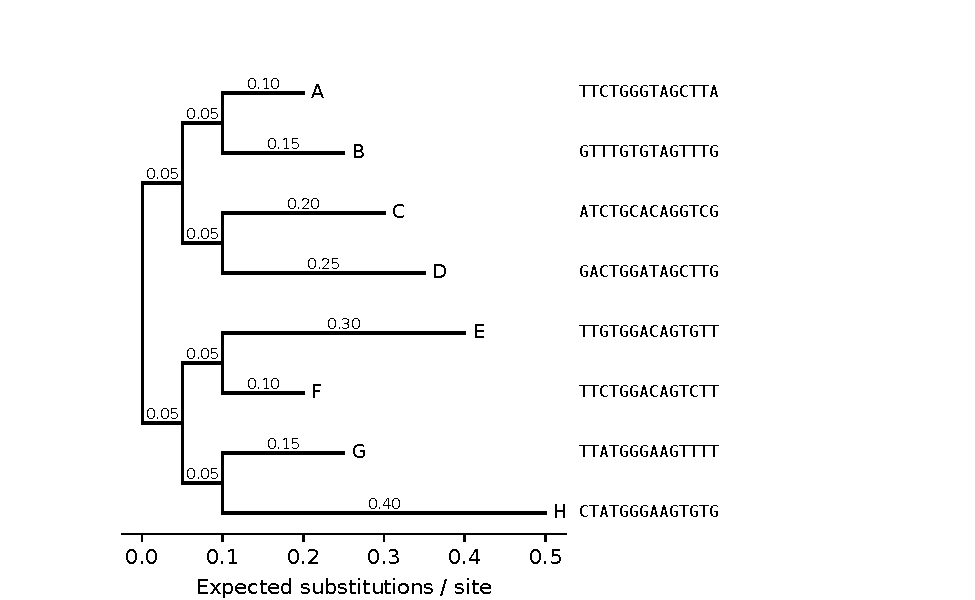
\includegraphics[width=0.7\linewidth]{figures/sim_tree}
  \caption{\simTreeCaption}
  \label{fig:sim-tree}
\end{figure}

\qacaptionread{figures/jc_transition_caption.txt}{\jcTransitionCaption}
\begin{figure}[htbp]
  \centering
  \includegraphics[width=0.7\linewidth]{figures/jc_transition}
  \caption{\jcTransitionCaption}
  \label{fig:jc-transition}
\end{figure}

\subsection{The algorithm: simulation}
The generative direction of Equation~\ref{eq:site-independence} is a pre-order
walk: draw the root state, then each node's state from the row of its parent's
state. One site is Algorithm~\ref{alg:simulate}; $L$ sites are $L$ independent
runs, and the empirical substitution frequencies along any branch converge to
Equation~\ref{eq:jc}, the check a simulator is held to---against the closed
form, never against the likelihood later fitted to its output.

\begin{algorithm}[htbp]
\caption{Forward simulation of one site under $(\tree, \branch, \Q)$}
\label{alg:simulate}
\begin{algorithmic}[1]
\State draw $z_{\rootnode} \sim \bpi$
\For{each non-root node $v$ in pre-order, with parent $u$}
  \State draw $z_v \sim \Pmat_{z_u,\,\cdot}(\tau_v)$
\EndFor
\State \Return the leaf states $(z_\ell)_{\ell \in \mathrm{leaves}(\tree)}$
\end{algorithmic}
\end{algorithm}

\subsection{The algorithm: pruning}
Felsenstein's pruning evaluates that marginal in $O(n L k^2)$ rather than
$O(L k^{n-2})$, by a post-order recursion carrying a partial likelihood
$L_u(i)$---the probability of the data below node $u$ given that $u$ is in
state $i$:
\begin{equation}
  L_u(i) = \prod_{v \in \mathrm{children}(u)}
           \sum_{j \in \states} \Pmat_{ij}(t_v)\, L_v(j),
  \label{eq:pruning}
\end{equation}
with $L_u(i) = \mathbb{1}[\,\text{$u$ observed in state $i$}\,]$ at a leaf, and
the site likelihood read off at the root,
\begin{equation}
  p(\data_s \mid \tree, \branch, \Q) = \sum_{i \in \states} \pi_i\, L_{\rootnode}(i)
  \label{eq:root}
\end{equation}
\citep{felsenstein2004, durbin1998}; Appendix~\ref{app:pruning} derives the
recursion from the marginalization. Products of many small numbers underflow,
so each node's partials are rescaled and the logarithm of the scaling
accumulated separately; the rescaling must remain differentiable, since
$\branch$ and $\Q$ are what the continuous optimization fits.

\paragraph{Site patterns.}
Equation~\ref{eq:site-independence} reads one column per term, so two
identical columns contribute identical terms and the sum over $L$ columns is
a weighted sum over the $P \le \min(L, k^{\,n})$ distinct ones:
\begin{equation}
  \ell(\tree, \branch)
    = \sum_{s=1}^{L} \log p(\data_s \mid \tree, \branch, \Q)
    = \sum_{p=1}^{P} w_p \, \log p(\data_p \mid \tree, \branch, \Q),
  \qquad \sum_p w_p = L,
  \label{eq:site-patterns}
\end{equation}
with $w_p$ the number of columns equal to pattern $p$. The identity is exact:
the arithmetic is reassociated, not approximated, and only the floating-point
summation order distinguishes the two sides. It is the standard first step of a
maximum-likelihood implementation \citep{felsenstein2004}, and it saturates,
since $P \le k^{\,n}$ however long the alignment---at $k = 4$ and four taxa
$P \le 256$ whatever $L$ is. Compression is a property of the alignment rather
than of an evaluator, so every backend consumes patterns and weights.

Equation~\ref{eq:pruning} is Equation~\ref{eq:sum-product} run leaf to root
with the root as the last variable: $L_u(i)$ is the product over $u$'s
children of the factor-to-variable messages $m_{\psi_v \to u}(i)$, each of
which sums the branch factor against the message arriving from below, and
Equation~\ref{eq:root} is the final factor-to-variable message from the
prior. Replacing the sum by a maximum gives the most probable joint assignment
of ancestral states; in the limit of short branches its cost counts
substitutions, which is Fitch parsimony \citep{felsenstein2004}, the second
criterion the search is scored against.

Both parsimony scores are the same post-order pass with no branch lengths.
Fitch's recursion \citep{fitch1971} carries at each node $v$ the set $S_v$
of states reachable at the minimum cost so far, and a count $F$ of changes:
\begin{equation}
  S_v = \begin{cases}
    S_a \cap S_b & S_a \cap S_b \neq \emptyset, \\
    S_a \cup S_b \quad\text{and}\quad F \leftarrow F + 1 & \text{otherwise},
  \end{cases}
  \label{eq:fitch}
\end{equation}
for the children $a, b$ of $v$, folded pairwise at a trifurcation, a leaf's
set being its observed state. Sankoff's recursion \citep{sankoff1975}
replaces the set by a cost vector under a step matrix $W \in
\mathbb{R}_{\ge 0}^{k \times k}$, $W_{ij}$ the cost of a change from a
parent in state $i$ to a child in state $j$:
\begin{equation}
  S_v(i) = \sum_{c \in \mathrm{ch}(v)} \min_j \big[\, W_{ij} + S_c(j) \,\big],
  \qquad
  S_{\mathrm{leaf}}(i) = \begin{cases} 0 & i = x_{\mathrm{leaf}}, \\
    \infty & \text{otherwise}, \end{cases}
  \label{eq:sankoff}
\end{equation}
and a site's score is $\min_i S_{\mathrm{root}}(i)$.
Equation~\ref{eq:pruning} in the min-plus semiring, returning Fitch's count
exactly under the unit matrix $W = \mathbf{J} - \mathbf{I}$. The score is a
rooted tree's: an asymmetric $W$ scores each rooting of one unrooted topology
differently, so a search over unrooted topologies is well defined only when
$W$ is a metric, where every rooting agrees.

\paragraph{The gradient in the branch lengths.}
Fitting $\branch$ needs $\partial \ell / \partial t_v$ for all $2n-3$ branches.
Differentiating Equation~\ref{eq:pruning} branch by branch costs one recursion
each; a single root-to-tip pass returns all of them together, the transpose of
the post-order pass rather than a second algorithm \citep{felsenstein2004}.
Write $A^s_u(i) = \partial \ell / \partial L^s_u(i)$
for the adjoint of node $u$'s partial at site $s$, $m^s_v(i) = \sum_j
\Pmat_{ij}(t_v)\, L^s_v(j)$ for the message $v$ sends its parent, and
$\dot{\Pmat}(t) = \mathrm{d}\Pmat/\mathrm{d}t$, which is closed form under
Equation~\ref{eq:jc} and $\Q\,\Pmat(t)$ in general. Equation~\ref{eq:root}
starts the pass,
\begin{equation}
  A^s_{\rootnode}(i) = \frac{\pi_i}{\sum_{j \in \states} \pi_j\, L^s_{\rootnode}(j)},
  \label{eq:adjoint-root}
\end{equation}
and for a non-root node $v$ with parent $u$, abbreviating
$B^s_v(i) = A^s_u(i) \prod_{w \in \mathrm{children}(u) \setminus \{v\}} m^s_w(i)$,
\begin{equation}
  \frac{\partial \ell}{\partial t_v}
    = \sum_{i,j \in \states} \dot{\Pmat}_{ij}(t_v) \sum_s B^s_v(i)\, L^s_v(j),
  \qquad
  A^s_v(j) = \sum_{i \in \states} B^s_v(i)\, \Pmat_{ij}(t_v),
  \label{eq:pruning-backward}
\end{equation}
which is Algorithm~\ref{alg:pruning-backward}. Its cost is $O(n L k^2)$, the
forward pass's, and independent of the number of branches differentiated.

Two properties of that pass are places an implementation goes wrong silently.
First, the rescaling contributes nothing: $\ell$ is algebraically independent
of the per-node scales, the divided partial and the accumulated logarithm
moving against each other, so the derivative may be taken with the scales
frozen at the forward pass's values and each adjoint divided by its own node's
scale. Second, the sibling product $\prod_{w \neq v} m^s_w$ must be formed by a
scan over the siblings and not as $L^s_u / m^s_v$: a message vanishes at any
site whose observation forbids that state, where the quotient is $0/0$ and the
derivative is finite.

\begin{algorithm}[htbp]
\caption{Two-pass gradient of the pruning recursion in the branch lengths}
\label{alg:pruning-backward}
\begin{algorithmic}[1]
\State run Equation~\ref{eq:pruning} in post-order, keeping each node's
       partial $L^s_v$ and the message $m^s_v$ it sent its parent
\State $A^s_{\rootnode} \gets \bpi \,/ \sum_{j} \pi_j L^s_{\rootnode}(j)$
       \Comment{Equation~\ref{eq:adjoint-root}}
\For{each non-root node $v$ in pre-order, with parent $u$}
  \State $B^s_v(i) \gets A^s_u(i) \prod_{w \in \mathrm{children}(u) \setminus \{v\}} m^s_w(i)$
  \State $\partial \ell / \partial t_v \gets \sum_{i,j} \dot{\Pmat}_{ij}(t_v) \sum_s B^s_v(i) L^s_v(j)$
  \State $A^s_v(j) \gets \sum_i B^s_v(i)\, \Pmat_{ij}(t_v)$
\EndFor
\State \Return $(\partial \ell / \partial t_v)_{v \neq \rootnode}$
\end{algorithmic}
\end{algorithm}

\paragraph{Regime.}
Exact on every input, a tree having no cycle. The one failure mode is
numerical---underflow of a product of $n$ factors each below one---and the
rescaling removes it rather than tolerating it.

\paragraph{What pins it.}
Direct marginalization, Equation~\ref{eq:site-independence}, at the sizes it
allows, to a relative tolerance (Section~\ref{sec:tolerance}). Two invariants
past those sizes: the pulley principle, that a reversible model's likelihood
does not depend on where the root is placed along a branch, and a gradient
against central differences relative to its own norm---which refereed
Algorithm~\ref{alg:pruning-backward} against the same likelihood differentiated
by a tape, the two agreeing to a tighter tolerance than either agrees with the
difference quotient. And the recovery test of Section~\ref{sec:properties}: on
simulated data the fitted branch lengths cover the truth at their nominal rate,
and the search recovers the generating topology at a stated site count.

\subsection{The algorithm: discrete search}
The number of unrooted binary topologies on $n$ taxa is $(2n-5)!!$
\citep{rosen2019}, so exhaustive enumeration is an oracle at small $n$ and
nothing more. Two neighbourhoods are standard. \emph{Nearest-neighbour
interchange} (NNI) swaps the subtrees adjacent to one internal edge, giving
$|\neighbourhood_{\mathrm{NNI}}(\tree)| = 2(n-3)$. \emph{Subtree prune and
regraft} (SPR) detaches a subtree and reattaches it at another edge, giving
$2(n-3)(2n-7)$ and containing NNI. Neither is complete in one step; both are
complete in the transitive closure, which for NNI is the connectivity of the
associated graph \citep{felsenstein2004} and is inherited by SPR because it
dominates NNI.

Hill climbing over either neighbourhood fits the continuous parameters of every
candidate and moves to the best; its budget is counted in candidates scored,
never in seconds, so a run reproduces from its seed. The same climb with
Equation~\ref{eq:fitch} or~\ref{eq:sankoff} in place of the fit is \emph{large
parsimony} \citep{felsenstein2004}: nothing continuous is fitted, a candidate
costs one pass, and the budget and the oracle are the same. A candidate sharing
all but a few branches with its parent may start its fit from the parent's
lengths, a branch identified by the leaf bipartition below it rather than by a
node's name; and a neighbourhood may be \emph{ranked} by one evaluation at
those lengths before the few best are fitted, the accepted move always in full,
so every reported score is an optimum. Whether the ranking finds the fitted
best is measured per move set, not assumed.

Three further economies apply to the same climb, each separable from the
others. The climb may begin at a most-parsimonious topology, since a parsimony
pass costs no fit. The regraft may be bounded
to edges within distance $r$ of the vacated edge, giving
$|\neighbourhood_{\mathrm{SPR}}^{r}(\tree)| = O(nr)$ in place of $O(n^2)$;
$r=1$ is exactly the NNI neighbourhood, so a bounded SPR inherits NNI's
transitive completeness at every $r$, and $r$ at least the tree's diameter is
SPR itself. And a candidate may be fitted over only the branches whose
bipartition the move changed --- the path between the vacated and the graft
edge, one edge under NNI --- holding the rest at the parent's fitted lengths.
That last optimizes over a subspace, so its value lower-bounds the candidate's
maximum rather than equalling it: it decides which candidate to accept, and the
accepted one is refitted over every branch, as a ranked neighbourhood is.

\paragraph{What pins it.}
Enumeration of the $(2n-5)!!$ topologies referees the search below eight taxa:
the climb must reach the enumerated maximum, and the neighbourhood counts
above are asserted exactly over every topology. Each economy is held to that
same enumeration alone and in combination, or the rate at which it loses the
optimum is measured and stated. Two also have an exact reduction to something
already refereed, which a count alone would not catch: the bounded regraft at
$r=1$ must equal the NNI neighbourhood, and at $r$ past the diameter the
unbounded one, candidate for candidate. A warm start is pinned by reaching the
cold fit's optimum; a cached partial likelihood by equalling the recomputed one
bitwise, being the same arithmetic in the same order. Large parsimony is held
to the same enumeration from every start, and on the Felsenstein-zone fixture
its enumerated optimum is asserted to be the wrong tree while the likelihood
optimum is the right one, since there the criterion's failure is the theorem of
Section~\ref{sec:properties} and not a defect of the search.

\subsection{The initializer: distances, neighbor joining and the Hadamard spectrum}
\label{sec:spectral-start}
Spectral learning of a hidden Markov model \citep{hsu2012} is a method of
moments: the observable moments of short windows are inverted to the
parameters, with a consistency guarantee and no likelihood surface to climb.
\citet{mossel2006} carry the argument to a phylogeny---the same inversion of
pairwise moments learns a nonsingular tree---where it becomes a distance per
pair of taxa and a tree from the distances.
The pair co-occurrence matrix $F$ of two taxa, $F_{ij}$ the fraction of sites
at which the first is in state $i$ and the second in $j$, is the moment;
under Equation~\ref{eq:jc} its off-diagonal mass is $\tfrac{k-1}{k}(1 -
e^{-kt/(k-1)})$ for $t$ the path length between the two, which inverts in
closed form on the fraction $p$ of differing sites,
\begin{equation}
  \hat d = -\frac{k-1}{k}\,\log\!\Big(1 - \frac{k}{k-1}\,p\Big),
  \qquad
  \operatorname{Var}(\hat d) = \frac{p\,(1-p)}{L\,(1 - \tfrac{k}{k-1}p)^2},
  \label{eq:jc-distance}
\end{equation}
the variance by the delta method over the multinomial site counts. Under
a general Markov process on the branches the log-det distance
\citep{steel1994}
\begin{equation}
  \hat d = -\frac{1}{k}\Big[\log\det F
    - \tfrac12\big(\log\det \Pi_x + \log\det \Pi_y\big)\Big],
  \label{eq:logdet}
\end{equation}
$\Pi_x, \Pi_y$ the diagonal matrices of $F$'s row and column sums, is
additive along the tree whatever the process; it equals $t$ when $\Q$ has
trace $-k$, which Equation~\ref{eq:normalization} gives the Jukes--Cantor
model, and $-\operatorname{tr}(\Q)\,t/k$ under a general reversible $\Q$,
a constant that leaves the tree unchanged.

Neighbor joining \citep{saitou1987} is the tree from the distances,
Algorithm~\ref{alg:neighbor-joining}: $n-3$ agglomerations of the pair
minimizing $(n-2)\,d_{ij} - r_i - r_j$, $r$ the row sums, each placing the
new node by the three-point formula and reducing the matrix by one. On an
additive matrix---one whose entries are the path lengths of some tree---it
returns that tree with every branch length exact, and whether a matrix is
additive is the four-point condition: of the three sums $d_{ij}+d_{kl}$,
$d_{ik}+d_{jl}$, $d_{il}+d_{jk}$ over any four taxa, the two largest are
equal \citep{felsenstein2004}. On an estimated matrix \citet{atteson1999}
gives the guarantee: the topology is the true one whenever every entry's
error is below half the shortest branch, and Equation~\ref{eq:jc-distance}'s
variance is what lets a run state whether it sits inside that radius.

\begin{algorithm}[htbp]
\caption{Neighbor joining on a distance matrix $D$ over $n$ taxa}
\label{alg:neighbor-joining}
\begin{algorithmic}[1]
\While{more than three nodes remain}
  \State $r_i \gets \sum_j D_{ij}$ for every remaining node $i$
  \State $(i, j) \gets \arg\min_{i \neq j}\, (n-2)\,D_{ij} - r_i - r_j$
  \State join $i$ and $j$ at a new node $u$ with
    $D_{iu} = \tfrac12 D_{ij} + \tfrac{r_i - r_j}{2(n-2)}$,\;
    $D_{ju} = D_{ij} - D_{iu}$
  \State $D_{ku} \gets \tfrac12 (D_{ik} + D_{jk} - D_{ij})$ for every other $k$;
    remove $i$ and $j$; $n \gets n - 1$
\EndWhile
\State join the last three at the root by the three-point formula
\end{algorithmic}
\end{algorithm}

For the symmetric two-state model the inversion is exact rather than
pairwise. \citet{hendy1993} index the $2^{n-1}$ site patterns by the set of
taxa differing from a reference taxon, and the same subsets index the splits
of the leaf set; with $s$ the pattern frequencies and $q$ the branch length on
each split, zero where the tree has no such branch, the two are conjugate
under the Sylvester--Hadamard matrix $\hadamard$ of that order,
\begin{equation}
  s = \hadamard^{-1} \exp(\hadamard q), \qquad q = \hadamard^{-1} \log(\hadamard s),
  \label{eq:hadamard}
\end{equation}
so the exact spectrum returns the tree's own lengths on its splits and zero
elsewhere. The \emph{closest tree}, Algorithm~\ref{alg:hadamard-start}, takes
the $n-3$ largest mutually compatible weights of an estimated $q$. A four-state
Jukes--Cantor alignment reduces to the two-state model exactly by grouping the
states in pairs, at $\tfrac{2}{3}$ of every branch length; the four-state
conjugation is over the Klein four-group and is not implemented. Both
estimators are a start and not an estimate: the fit and the search begin from
them, and every reported number is the optimum they reach.

\paragraph{What pins it.}
Equation~\ref{eq:jc-distance} against Equation~\ref{eq:jc} at the exact pair
frequencies; Equation~\ref{eq:logdet} against $t$ under Jukes--Cantor and
against $-\operatorname{tr}(\Q)\,t/k$ under a general reversible $\Q$; the
stated variance by the coverage of its interval over seeds. Neighbor joining
against the path lengths of every fixture and of random trees at 20 and 50
taxa, every branch to $10^{-12}$; on simulated alignments, recovery on every
replicate inside Atteson's radius, with no exception. The Hadamard
conjugation against the pruning likelihood of Section~\ref{sec:phylo}
evaluated on every pattern, which shares nothing with the transform. And the
starts against the objective's own, at equal evaluations, through the
budgeted comparison of Section~\ref{sec:properties}.

\subsection{The relaxation: the tropical Grassmannian}
\label{sec:tropical}
The four-point condition of Section~\ref{sec:spectral-start} is more than a
test for additivity: it is the defining relation of a variety.
\citet{speyer2004} show that the tropical Grassmannian $\mathrm{Gr}(2,n)$, the
tropicalization of the Pl\"ucker relations for two-planes in $n$-space, is the
space of trees on $n$ leaves --- its points the vectors
$d \in \mathbb{R}^{\binom{n}{2}}$ for which every quartet's largest pairing sum
is attained twice. Two consequences make it a relaxation of topology search.
The coordinates are continuous, so a tree is a point of a Euclidean space; and
a quartet's resolution is the pairing attaining the \emph{smallest} of its
three sums, so the discrete structure is an $\arg\min$ of a linear function of
those coordinates.

Relaxing the $\arg\min$ relaxes the topology. Write $s_Q(d) \in \mathbb{R}^3$
for the pairing sums of quartet $Q$ and $\ell_Q \in \mathbb{R}^3$ for a score
per resolution --- the maximized log-likelihood of the four-taxon tree, say.
The softmin at temperature $\tau$ gives
\begin{equation}
  F_\tau(d) \;=\; \sum_Q \big\langle
    \operatorname{softmax}(-s_Q(d)/\tau),\; \ell_Q \big\rangle,
  \label{eq:tropical-relaxation}
\end{equation}
differentiable in $d$ throughout and linear in the softmin weights, so at a
one-hot weight vector it equals the discrete objective
$D(\tree) = \sum_Q \ell_Q[r_\tree(Q)]$ exactly: an extension of what it relaxes
rather than a second model, the demand Section~\ref{sec:properties} also makes
of the Gumbel-softmax relaxation of a discrete state space.

Three properties bound what may be claimed for it, and each is checkable.
\emph{The scale of $d$ is a gauge}: $F_\tau(c\,d) = F_{\tau/c}(d)$ for
$c > 0$, so an unconstrained ascent maximizes $F$ by inflating the metric ---
sharpening the softmin --- without moving a single resolution, and $d$ must be
normalized for $\tau$ to be the only sharpness. \emph{The corner agreement is
a derived tolerance, not a constant}: with $g_Q$ the gap between a corner's
smallest and second-smallest pairing sum and $R_Q$ the range of $\ell_Q$, the
softmin leaves at most $2\exp(-g_Q/\tau)$ weight off the corner's own
resolution, so
\begin{equation}
  \big| F_\tau(d) - D(\tree) \big| \;\le\; \sum_Q 2\,e^{-g_Q/\tau}\,R_Q,
  \label{eq:tropical-corner}
\end{equation}
which inverts for the $\tau$ any requested tolerance needs and shrinks with a
fixture's shortest internal branch. \emph{The relaxation is outer}: $F_\tau$ is
defined on all of $\mathbb{R}^{\binom{n}{2}}$ and not on $\mathrm{Gr}(2,n)$, a
general dissimilarity resolves every quartet, and the resolutions need not come
from any tree. Ascent may leave the variety, and the topology is read off the
point it stops at by neighbor joining, exact on the variety.

$D$ is a quartet decomposition of the criterion and not the tree's
log-likelihood --- a different surface, so substituting one for the other is
licensed by measuring that the two agree at the $\arg\max$, never by a
correlation.

\paragraph{What pins it.}
Equation~\ref{eq:tropical-relaxation} against $D$ at the metric of every
enumerated topology, relatively --- the residual once
Equation~\ref{eq:tropical-corner} is under an absolute bound is float64
rounding of a sum over $\binom{n}{4}$ terms, which does not transfer between
problem sizes. The $\arg\min$ reading of a quartet against the tree's own leaf
bipartitions, which share no arithmetic. Equation~\ref{eq:hadamard} on the
exact two-state spectrum, whose edge weights sum over separating splits to a
metric that must satisfy the four-point condition and resolve every quartet as
the tree does --- a route to a point of $\mathrm{Gr}(2,n)$ that shares no
algebra with a walk over the tree. The $\arg\max$ of $D$ against the
$\arg\max$ of the fitted likelihood, enumerated. And ascent against the
enumerated maximum of $D$, or, where a fixture's top two topologies lie
within the convergence of the fits that scored them, against the generating
topology instead, since a ranking that turns on less than the optimizer's
convergence is not a property of the model.

\subsection{Choosing among these at the supported sizes}
\label{sec:phylo:discussion}
Four algorithms are assumed rather than derived here: the post-order
marginalization (Appendix~\ref{app:pruning}), the two-pass adjoint that
differentiates it (Algorithm~\ref{alg:pruning-backward}), the agglomeration
building a tree from a distance matrix (Algorithm~\ref{alg:neighbor-joining}),
and the climb over a neighbourhood (Algorithm~\ref{alg:hill-climbing}). Each is
standard and stated in the appendix. Citing them does not settle which to spend
a budget on at a given taxon count; Table~\ref{tab:phylo:regimes} answers that.

\begin{table}[htbp]
  \centering
  \footnotesize
  \begin{tabular}{@{}p{0.13\textwidth}p{0.24\textwidth}p{0.55\textwidth}@{}}
    \toprule
    Taxa & What referees & What to run, and why not the alternative \\
    \midrule
    5--6 & Enumeration, 15 and 105 topologies
      & The climb is run to be \emph{scored}, not to find. Ranking a
        neighbourhood by a surrogate buys nothing: the neighbourhood is
        smaller than the number of fits the ranking saves. \\
    7--8 & Enumeration, 945 and 10{,}395
      & Enumeration is still the referee but now costs one continuous fit
        per candidate, so the climb is what is run and the enumeration what
        scores it. Parsimony reaches the same neighbourhood for one pass
        per candidate instead of one optimization. \\
    9--12 & Nothing exhaustive; the two-state spectrum, $2^{n-1}$ entries
      & The exact conjugation is the only start with an argument behind it
        rather than a measurement, and it is the last size at which one
        exists. A likelihood optimum here is reported and not certified. \\
    13--200 & Additivity, and the radius an estimated matrix must sit
        inside
      & Distances and the agglomeration are the start; the climb reports
        the optimum it reached. Whether that is the optimum is not
        established, and the one surviving statement is the radius --- which
        the variance of Equation~\ref{eq:jc-distance} says whether a run is
        inside. \\
    to 1000 & Recovery of the generating tree, or nothing
      & Only the evaluation is affordable, at $O(n L k^2)$ a pass. The
        search is unrefereed, and closing it needs a bound on the optimum
        rather than a faster climb --- the cell
        Section~\ref{sec:applicability} marks. \\
    \bottomrule
  \end{tabular}
  \caption{What referees a phylogenetic claim at each taxon count, and what
  that leaves worth running. The taxon count and not the alignment length is
  the axis, for the reason the paragraph below gives.}
  \label{tab:phylo:regimes}
\end{table}

The alignment length is a second axis and behaves oppositely. Pattern
compression saturates at $P \le k^{\,n}$ (Equation~\ref{eq:site-patterns}), so
past a few thousand sites an evaluation stops growing in cost while the
estimate keeps sharpening: length is the cheapest resolution on offer, and the
reason the declared range reaches eleven thousand sites at a taxon count whose
search is unrefereed. Below a few hundred sites the same variance decides
whether a distance matrix sits inside the recovery radius at all.

\paragraph{What each method needs of the model.}
The recursion applies to any tree and any rate matrix, reversible or not. The
closed form Equation~\ref{eq:jc} is Jukes--Cantor's alone; the log-det
distance, Equation~\ref{eq:logdet}, is additive under any Markov process on the
branches and is the one distance surviving a model the fit does not assume. The
conjugation of Equation~\ref{eq:hadamard} is the symmetric two-state model's,
reaching four states only through the exact pairing reduction. The tropical
relaxation applies wherever a quartet carries a score, but is \emph{outer}:
ascent may leave the space of trees, so it is a way of moving and never of
reporting, and the topology is read back by an algorithm exact on the space.

\paragraph{What the validation assumes.}
Three application-specific properties, and every referee in
Section~\ref{sec:phylo:validation} rests on one. Sites are independent and
identically distributed given the tree, which makes direct marginalization a
per-column sum and pattern compression an identity. The model is
time-reversible, which is the whole content of the pulley principle: the
invariant is a statement about $\Q = \SubMat \operatorname{diag}(\bpi)$ and is
silent about a model that is not reversible. And recovery assumes the data came
from the model, so it calibrates the pipeline on its own samples and transfers
to nothing else --- the referee of last resort.

\subsection{Validation}
\label{sec:phylo:validation}
Each referee below establishes one thing and is silent about the rest; the list
is what the section may claim.
\begin{itemize}
  \item \emph{Direct marginalization} over the $k^{\,n-2}$ internal
    assignments, Equation~\ref{eq:site-independence}, shares no traversal
    with Equation~\ref{eq:pruning} and establishes that the recursion computes
    the marginal it claims, to a relative tolerance. It does not reach past the
    taxon count the supported sizes give, and says nothing about the rescaling
    at lengths where the unscaled product would underflow.
  \item \emph{The closed form} Equation~\ref{eq:jc} referees the simulator
    through the empirical substitution frequencies along a branch. It
    establishes that the generative direction is the model; it does not check
    the likelihood, since a simulator checked against the evaluator fitted to
    its output referees nothing.
  \item \emph{The pulley principle} --- a reversible model's likelihood is
    unchanged by where the root sits along a branch --- and the gradient
    against central differences hold past every enumerable size. They are
    invariants, not answers: both are satisfied by a wrong likelihood that is
    wrong reversibly.
  \item \emph{Topology enumeration} of the $(2n-5)!!$ candidates referees the
    search, which must reach the enumerated maximum, and the neighbourhood
    counts $2(n-3)$ and $2(n-3)(2n-7)$ are asserted exactly over every
    topology. Past those sizes nothing here says the climb succeeded, which
    is what a branch-and-bound bound would supply.
  \item \emph{Recovery of the simulated truth} --- the generating topology at a
    stated site count, and branch lengths covered by their intervals at the
    nominal rate --- is the referee where no oracle reaches. It establishes
    that the pipeline is calibrated on data from its own model and nothing
    about data the model does not describe.
  \item \emph{The path lengths of a known tree} referee neighbor joining
    exactly on an additive matrix, and Atteson's radius bounds when an
    estimated matrix still recovers the topology. Outside that radius the
    start is a start and not an estimate, and only the fit that follows it is
    reported.
\end{itemize}

\subsection{Extensions, and what is not attempted}
\label{sec:phylo:extensions}
\paragraph{What it would take to go further.}
The gap is the one Table~\ref{tab:phylo:regimes}'s last row names: past the
enumerable taxon count nothing says a climb found the optimum. What closes it
is a \emph{bound}, not a faster climb --- a branch and bound over the topology
space, with Equation~\ref{eq:parsimony-bound} or the plug-in of
Equation~\ref{eq:plugin-bound} pruning a subtree of the search
\citep{papadimitriou1998}. Three further directions each have a prerequisite. A
posterior over topologies rather than a flat-prior weight over maximized
likelihoods needs a chain that mixes over the move graph, whose mixing is
studied rather than assumed \citep{whidden2015, altekar2004}; a differentiable
topology needs a parameterization of the space itself, which the subsplit
constructions supply and which would give Section~\ref{sec:tropical} an oracle
it lacks \citep{zhang2018, zhang2019}; and a learned ranking of the regraft
neighbourhood is the surrogate Section~\ref{sec:surrogates} ranks with, learned
rather than derived \citep{azouri2021}. Richer substitution models --- rate
heterogeneity across sites, a general time-reversible matrix fitted rather than
fixed --- change the evaluator's parameter vector and nothing about its
referees \citep{yang2014}. Established implementations are a comparison not
made here \citep{minh2020, kozlov2019}: they are surveyed, and admitting one is
a decision on its own evidence.

\paragraph{What is deliberately not attempted.}
Empirical alignments, since there is no true tree behind one and a result on it
can be reported but not refereed --- the reason every fixture is simulated.
Model misspecification, since every recovery statement here is calibration on
the model's own samples. Insertions and deletions, which break the site
independence every referee in Section~\ref{sec:phylo:validation} rests on and
would need a different likelihood rather than a longer one. And the four-state
Hadamard conjugation over the Klein four-group: the two-state transform with
the exact pairing reduction is carried, the general one stated and left
unbuilt.

\section{Problem Statement: Potts Models in an External Field}
\label{sec:potts}

\subsection{The model}
\label{sec:potts:model}
On a graph $\graph$, each node $i$ carries a spin $\sigma_i \in \{1, \dots, q\}$
and the energy is
\begin{equation}
  \energy(\sigma) = -\sum_{\langle i,j \rangle} J_{ij}\,\delta(\sigma_i, \sigma_j)
                    - \sum_i h_i(\sigma_i),
  \label{eq:potts}
\end{equation}
with couplings $J_{ij}$ and an external field $h_i$ \citep{mezard2009}. The
Boltzmann distribution is $p(\sigma) \propto \exp(-\energy(\sigma))$, and its
normalizer sums over $q^{|V|}$ configurations.

\paragraph{Supported sizes.}
\label{par:potts:sizes}
The exact referee is the $q^{|V|}$ enumeration, refused past 200,000
configurations, which puts the ceiling at eleven nodes at three states and
seventeen at two. The fixtures sit under it: a chain of twelve sites at three
states over 400 replicates, and two open $3 \times 3$ lattices at three
states, one in a shared field and one in a per-site field, whose
$3^9 = 19{,}683$ configurations give the exact normalizer and every marginal.
Above it the transfer matrix referees a strip of any length at a width that
fits --- which is where the $12 \times 6$ per-site-field instance sits, at
$3^{72}$ configurations --- belief propagation is compared on the
$8 \times 8$ lattice where nothing is exact, the minimum cut is checked at
extents 8, 12 and 16, and the cluster moves are separated from single-site
sweeps at extents 8 and 24, the $12 \times 12$ of them at the square-lattice
transition of Section~\ref{sec:potts-sampling} being a declared instance. The
largest per-site-field instance is a triangular $71 \times 71$ at ten states,
5,041 nodes, where no normalizer is available at any cost and what is asserted
is that the covariate still tilts the labels. The general graph carries
$G(n, p)$ instances to a hundred nodes, refereed by the planted energy of
Section~\ref{sec:frustrated} rather than by any enumeration.

\subsection{As a factor graph}
The variables are the spins, $x_i \equiv \sigma_i$. The factors are one unary
$\psi_i(\sigma_i) = e^{h_i(\sigma_i)}$ per node and one pairwise
$\psi_{ij}(\sigma_i, \sigma_j) = e^{J_{ij}\,\delta(\sigma_i, \sigma_j)}$ per
edge, so Equation~\ref{eq:factor-graph} is the Boltzmann distribution and $Z$
its normalizer. At a temperature $T$ the factors are raised to the power
$\beta = 1/T$, which is the same graph with $J$ and $h$ scaled; nothing else
about the model changes, and that is why a tempered chain can be held to the
unscaled model's enumeration. The graph is a tree exactly when $\graph$ is,
which is the regime every exact claim below is confined to.
Figure~\ref{fig:potts:sketch} is that structure on the square lattice.

% The Potts factor graph of Section~\ref{sec:potts}, drawn by hand. Input by
% textbook.tex; a sketch and not a rendered figure, so it is outside the
% figure cache and the render cap, which govern generated output only.
\begin{figure}[htbp]
\centering
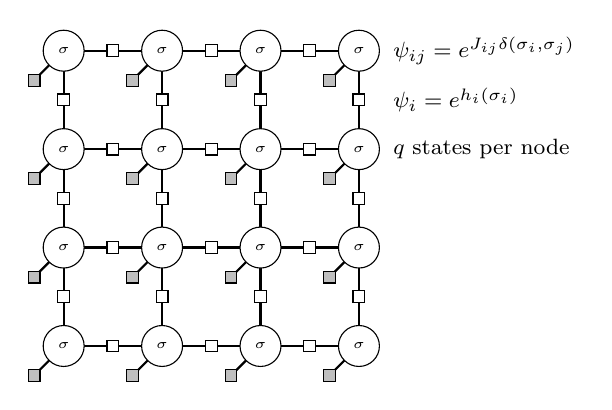
\begin{tikzpicture}[
    scale=1.25,
    spin/.style={circle, draw, minimum size=0.52cm, inner sep=0pt, font=\tiny, fill=white},
    factor/.style={rectangle, draw, fill=white, minimum size=0.15cm, inner sep=0pt},
    field/.style={rectangle, draw, fill=black!25, minimum size=0.15cm, inner sep=0pt},
    bond/.style={draw, thick}
]
  % Pairwise factors, one per edge of the open square lattice.
  \foreach \i in {0,...,3} {
    \foreach \j in {0,...,3} {
      \ifnum\i<3
        \draw[bond] (\i, \j) -- (\i+1, \j);
        \node[factor] at (\i+0.5, \j) {};
      \fi
      \ifnum\j<3
        \draw[bond] (\i, \j) -- (\i, \j+1);
        \node[factor] at (\i, \j+0.5) {};
      \fi
    }
  }
  % One field factor per node, on a stub so it is not mistaken for a bond.
  \foreach \i in {0,...,3} {
    \foreach \j in {0,...,3} {
      \draw[bond] (\i, \j) -- (\i-0.30, \j-0.30);
      \node[field] at (\i-0.30, \j-0.30) {};
      \node[spin] at (\i, \j) {$\sigma$};
    }
  }
  \node[anchor=west, font=\footnotesize] at (3.25, 3.0)
    {$\psi_{ij} = e^{J_{ij}\delta(\sigma_i,\sigma_j)}$};
  \node[anchor=west, font=\footnotesize] at (3.25, 2.5)
    {$\psi_{i} = e^{h_i(\sigma_i)}$};
  \node[anchor=west, font=\footnotesize] at (3.25, 2.0)
    {$q$ states per node};
\end{tikzpicture}
\caption{A Potts model in an external field as a factor graph, on the open
$4 \times 4$ square lattice. Circles are the spins $\sigma_i \in \{1, \dots,
q\}$; open squares on each edge are the pairwise factors of
Equation~\ref{eq:potts} and shaded squares on a stub are the unary field
factors. The graph has cycles, so Equation~\ref{eq:sum-product} on it is the
Bethe approximation of Equation~\ref{eq:bethe} and not the exact marginal;
the square lattice is two-colourable, so it also carries no frustration,
which is what Section~\ref{sec:frustrated} adds. A sketch of the structure
and not a rendering of any instance.}
\label{fig:potts:sketch}
\end{figure}


\subsection{Why an odd cycle is the whole story}
A two-state antiferromagnet ($J < 0$) wants every edge to disagree, possible
exactly when $\graph$ is $2$-colourable. So every bipartite lattice---a chain,
a square lattice---has a trivial ground state and says nothing about a hard
problem. Odd cycles make the ground state non-trivial, and where a counting
argument closes it fixes that ground state at every size: the difference
between a fixture that exercises an optimizer and one that does not.

\subsection{The algorithm: belief propagation}
Exact marginals come from enumeration at small sizes and from belief
propagation on a tree, where it is exact; on a loopy graph it is an
approximation whose accuracy is a property of the graph rather than of the
implementation \citep{koller2009, frey1998}. It is Equation~\ref{eq:sum-product}
with every factor pairwise or unary: composing the variable-to-factor message
with the unary factor gives the node-to-node form, in which the message from
$i$ to a neighbour $j$ is
\begin{equation}
  m_{i \to j}(\sigma_j) \;\propto\; \sum_{\sigma_i}
    \exp\!\big(J_{ij}\,\delta(\sigma_i,\sigma_j) + h_i(\sigma_i)\big)
    \prod_{l \in \partial i \setminus j} m_{l \to i}(\sigma_i),
  \label{eq:bp-message}
\end{equation}
iterated to a fixed point, with beliefs $b_i(\sigma_i) \propto e^{h_i(\sigma_i)}
\prod_{l \in \partial i} m_{l \to i}(\sigma_i)$ at a node and likewise on an
edge. The messages are carried in the logarithm and normalized every sweep: a
coupling of a few units on a small lattice already puts a product of
exponentials past what a linear recursion holds. The Bethe free energy of the
fixed point,
\begin{equation}
  F_{\mathrm{Bethe}}
    = \sum_{\langle i,j \rangle} \sum_{\sigma_i,\sigma_j}
        b_{ij}\,\big(E_{ij} + \log b_{ij}\big)
    + \sum_i \sum_{\sigma_i} b_i\, E_i
    - \sum_i (d_i - 1) \sum_{\sigma_i} b_i \log b_i,
  \label{eq:bethe}
\end{equation}
with $E_{ij} = -J_{ij}\,\delta(\sigma_i,\sigma_j)$, $E_i = -h_i(\sigma_i)$ and
$d_i$ the degree of $i$, equals $-\log Z$ exactly on a tree and approximates
it on a loopy graph \citep{yedidia2005, mezard2009}; Appendix~\ref{app:bethe}
states why, and Appendix~\ref{app:sum-product} places the tree case. A fixed
point the iteration never reached estimates nothing, so non-convergence is a
refusal rather than a number.

\paragraph{Regime.}
Exact on a tree, in two passes. On a loopy graph the flooding schedule is
iterated with damping to a tolerance and returns the Bethe approximation; the
tree schedule is refused rather than run, a number that looks exact and is not
being the worst output an evaluator can produce.

\paragraph{What pins it.}
On a tree, $\log Z$ and every marginal against enumeration to a stated relative
tolerance. On a loopy graph nothing asserts agreement with the truth---that
would assert something false---and what is asserted is the structure the
physics requires: exact at zero coupling, with a deviation from the exact
transfer matrix that grows away from it and is reported as a measurement.

\subsection{The algorithm: ground states as cuts}
\label{sec:potts-cuts}
With two states write $\sigma_i \in \{-1, +1\}$. The pairwise term of
Equation~\ref{eq:potts} is constant on agreeing edges and pays $J_{ij}$ on
disagreeing ones, so minimizing $\energy$ minimizes the weight of the
\emph{cut}---the set of edges whose endpoints differ---plus the field:
\begin{equation}
  \energy(\sigma) = \sum_{\langle i,j \rangle : \sigma_i \ne \sigma_j} J_{ij}
                    - \sum_i h_i(\sigma_i) + \text{const}.
  \label{eq:cut-energy}
\end{equation}
When every $J_{ij} \ge 0$ the pairwise term is submodular, the field becomes
a terminal edge to a source or a sink, and the ground state is a minimum
$s$--$t$ cut, exact by max-flow in polynomial time \citep{greig1989, clrs2022}.
When couplings are negative the problem is maximum cut, which is NP-hard; the
semidefinite relaxation rounded by a random hyperplane gives a cut whose
expected weight is at least $\alpha_{\mathrm{GW}} = 0.87856$ of the optimum,
\begin{equation}
  \mathbb{E}[\,w(\text{cut})\,] \;\ge\; \alpha_{\mathrm{GW}}\; \max_{\sigma} w(\sigma),
  \qquad
  \alpha_{\mathrm{GW}} = \min_{0 < \vartheta \le \pi}
    \frac{2}{\pi}\,\frac{\vartheta}{1 - \cos\vartheta},
  \label{eq:gw}
\end{equation}
and the relaxation's own value bounds the optimum from above
\citep{goemans1995}. The bound is the claim holding at every size; the realized
ratio on an instance is measured beside it and never quoted as the guarantee.

\paragraph{Regime.}
Exact where the couplings are submodular and refused rather than approximated
where they are not (Section~\ref{sec:properties}): a wrong ground state on a
structured instance is indistinguishable from a right one at any size worth
solving. The relaxation runs on any instance and certifies a ratio.

\paragraph{What pins it.}
Enumeration over $2^{|V|}$ configurations where it reaches; where it does not,
a \emph{reduction}: on a bipartite graph the maximum cut is every edge and on a
uniform ferromagnet the ground state is constant. A construction error in the
cut graph yields a merely worse labelling, which only a regime forcing the
general construction to reproduce a simpler validated one catches. A fixture
whose answer is trivial measures nothing, so the instances carry the odd cycles
of Section~\ref{sec:potts}.

\subsection{The algorithm: alpha expansion}
\label{sec:alpha-expansion}
With $q > 2$ states the ground state is NP-hard in general, and alpha
expansion approximates it by a sequence of exact two-state problems
\citep{boykov2001}. An \emph{expansion} on label $\alpha$ lets every site keep
its label or switch to $\alpha$; the best such move is the minimum cut of a
two-state graph built from the current labelling, exact when the pairwise term
is a metric on labels, which $\delta(\sigma_i, \sigma_j)$ is. Cycling over $\alpha$ until no expansion lowers the energy,
Algorithm~\ref{alg:alpha-expansion}, reaches a local minimum within a
constant of the global one,
\begin{equation}
  \energy(\hat\sigma) \;\le\; 2\,c\,\energy(\sigma^\star),
  \qquad
  c = \max_{\alpha \ne \beta'} d(\alpha, \beta') \big/ \min_{\alpha \ne \beta'} d(\alpha, \beta'),
  \label{eq:alpha-expansion}
\end{equation}
so a factor of two for the Potts metric, where $c = 1$. The guarantee assumes
each expansion is solved to optimality; where it is solved approximately the
certificate is optimistic, and only the symptom can be asserted---a value an
exact solve could not have produced.

\paragraph{What pins it.}
The two-label case must reproduce the exact minimum cut of
Section~\ref{sec:potts-cuts} exactly; enumeration referees the multi-label
case where it reaches; and the realized ratio against the enumerated optimum
is measured, since the bound is a theorem and the ratio is a number.

\subsection{The algorithm: sampling}
\label{sec:potts-sampling}
The single-site heat bath draws each spin from its conditional,
\begin{equation}
  p(\sigma_i \mid \sigma_{\partial i}) \;\propto\;
    \exp\!\Big(\beta \big[\textstyle\sum_{j \in \partial i} J_{ij}\,\delta(\sigma_i, \sigma_j) + h_i(\sigma_i)\big]\Big),
  \label{eq:heat-bath}
\end{equation}
one site at a time; a \emph{sweep} is one update of every site,
Algorithm~\ref{alg:heat-bath}. Near a
critical coupling correlated regions span the lattice and single-site moves
decorrelate slowly. On the square lattice that coupling is the self-dual
point $J_c = \ln(1 + \sqrt{q})$, and on the triangular lattice it is
$\ln(1 + v)$ for the positive root of $v^3 + 3v^2 = q$ \citep{baxter1982};
both are closed forms, so an instance meant to sit at one is placed there
rather than near it. Cluster moves flip such regions together
\citep{swendsen1987, wolff1989, newman1999}: in the Edwards--Sokal
representation \citep{edwards1988} a bond is placed between equal neighbours
with probability $1 - e^{-\beta J_{ij}}$, and each bond-connected cluster is
recoloured uniformly---every cluster at once in Swendsen--Wang, one cluster
grown from a random seed in Wolff. The bond construction is exact at zero
field only. In a field the recolouring is accepted with the Metropolis
probability on the field energy alone,
\begin{equation}
  a = \min\Big\{1,\ \exp\!\Big(\beta \textstyle\sum_{i \in \mathcal{C}}
      \big[h_i(\nu) - h_i(\mu)\big]\Big)\Big\},
  \label{eq:cluster-accept}
\end{equation}
for a cluster $\mathcal{C}$ recoloured from $\mu$ to $\nu$, which restores
detailed balance (Appendix~\ref{app:detailed-balance}).
Algorithm~\ref{alg:cluster-move} is the construction and
Algorithm~\ref{alg:parallel-tempering} the replica exchange of
Section~\ref{sec:tempering} over it.

\paragraph{Regime.}
Every move preserves the Boltzmann distribution at $\beta$, so a sweep may not
stop on a state-dependent condition: composing a \emph{number} of steps chosen
from the outcome biases toward the states that triggered the stop. The bond
probability is a probability only for $J_{ij} \ge 0$, and an antiferromagnet
has no like-spin clusters to flip, so the cluster moves refuse a negative
coupling rather than run badly.

\paragraph{What pins it.}
A sampler is validated by the distribution it converges to and never by
inspection: at an enumerable size the exact Boltzmann distribution is
available, and a chain is held to it by a goodness-of-fit test at a declared
significance, thinned by several autocorrelation times since successive sweeps
are not independent draws. The test's power is itself pinned---a move set with
the field accept step removed runs, mixes, and is rejected.

\subsection{Temperature, annealing and tempering}
\label{sec:tempering}
A temperature $T$ scales the model, $\energy / T$, so a chain at $T$ targets
$\exp(-\energy/T)$; a \emph{schedule} $T(t)$ over a budget of $t$ steps is one
object, shared by every consumer of it, with both endpoints reached exactly at
the declared steps and a step past the end refused. Simulated annealing is the
sampler on a decreasing schedule, returning the lowest-energy state seen
\citep{kirkpatrick1983}; at $T \to 0$ the heat bath is the argmin over each
site's conditional, which is iterated conditional modes, so annealing and
greedy descent are one search separated by the schedule alone.

Parallel tempering runs $R$ replicas at fixed temperatures $T_1 < \dots < T_R$
and, after each sweep, proposes to exchange the configurations of adjacent
replicas, accepting with
\begin{equation}
  a_{ij} = \min\big\{1,\ \exp\!\big[(\beta_i - \beta_j)(E_i - E_j)\big]\big\},
  \label{eq:exchange}
\end{equation}
the ratio of the joint target, a product of tempered marginals
\citep{swendsenwang1986, geyer1991, earl2005}; Appendix~\ref{app:exchange}
derives it. The hot replicas cross barriers the cold one cannot, and an
exchange carries what they find down the ladder. Each replica draws from its
own generator, spawned from one parent that draws only the exchange uniforms,
so no two replicas share a stream and one seed reproduces the run.

The replica at $T_1 = 1$ targets the unscaled model, so the fraction of its
$N$ recorded sweeps spent at a structure $x$ estimates that structure's
weight over the whole space,
\begin{equation}
  \hat{w}(x) = \frac{1}{N} \sum_{n=1}^{N} \big[\sigma_1^{(n)} = x\big]
  \;\to\; \frac{\exp(-\energy(x))}{Z},
  \label{eq:tempered-weight}
\end{equation}
where a weight over a neighbourhood is conditional on that neighbourhood and
enumeration is refused past its cap. The structure may be a labelling, a
hidden path, or a topology with $\energy$ the negative fitted log-likelihood,
where the limit is the flat-prior weight over maximized likelihoods and not a
marginal over branch lengths. It is a Monte Carlo estimate, named a posterior
weight only beside the exchange acceptance of every adjacent pair and the
autocorrelation time of the indicator, which say whether the ensemble mixed.

\paragraph{What pins it.}
Every replica's marginal must still be $\exp(-\energy/T_r)$, enumerated from
the \emph{unscaled} model, with exchanges on: a wrong exchange ratio
contaminates the cold replica with hot configurations and only that test says
so. Its power is pinned by the paired negative---an exchange omitting the
energy term still runs and still mixes, and is rejected on every replica.
Whether tempering or annealing beats restarts of descent at an equal budget of
sweeps is a property of the instance, measured on the frustrated,
past-enumeration instances the roadmap needs and never asserted in general.

\subsection{Choosing among these at the supported sizes}
\label{sec:potts:discussion}
Five algorithms are assumed and stated elsewhere: the message iteration and
the free energy of its fixed point (Appendices~\ref{app:sum-product}
and~\ref{app:bethe}), the minimum cut and the expansion cycle built on it
(Algorithm~\ref{alg:alpha-expansion}), the single-site and cluster updates
(Algorithms~\ref{alg:heat-bath} and~\ref{alg:cluster-move}), the replica
exchange over them (Algorithm~\ref{alg:parallel-tempering}), and the
semidefinite relaxation with its rounding. They are not alternatives in the
ordinary sense: a sampler estimates a distribution, a cut returns one
configuration, and message passing returns marginals and a free energy, so the
question being asked is what settles first. Scoring one against another's
referee is the standing error here.

\begin{table}[htbp]
  \centering
  \footnotesize
  \begin{tabular}{@{}p{0.26\textwidth}p{0.28\textwidth}p{0.38\textwidth}@{}}
    \toprule
    Instance & What is exact & What is worth running \\
    \midrule
    Tree-shaped graph, any size
      & Message passing, in two passes
      & Nothing else. Enumeration is affordable only where it is also
        unnecessary. \\
    Loopy, $q^{|V|}$ inside the enumeration ceiling
      & Enumeration: $\log Z$, every marginal, the ground state
      & Every method, and none of them for its answer --- this is where a
        method is scored rather than used. \\
    A strip at a width that fits, any length
      & The transfer matrix, for the normalizer
      & Message passing, whose deviation from it is the measurement that
        says what the loopy fixed point costs. \\
    Two states, every coupling non-negative
      & The minimum cut, in polynomial time at any size
      & The cut. A sampler run for a ground state here spends a budget on a
        solved problem. \\
    More than two states, couplings non-negative
      & Nothing
      & Expansion, whose factor-of-two bound
        (Equation~\ref{eq:alpha-expansion}) is a certificate where an
        optimum is unavailable; the realized ratio is measured beside it. \\
    Any negative coupling
      & Nothing
      & Single-site sampling, annealing and tempering --- the cut and the
        cluster moves refuse. Which of the three wins is a property of the
        instance, measured on Section~\ref{sec:frustrated}'s. \\
    Marginals past the enumeration ceiling
      & Nothing
      & Message passing alone, returning the Bethe approximation, which is
        reported and asserted against nothing. \\
    \bottomrule
  \end{tabular}
  \caption{What is exact on each kind of Potts instance and what is
  therefore worth a budget. The rows are instance properties and not sizes:
  above two states, or below zero coupling, a method is refused whatever the
  lattice extent.}
  \label{tab:potts:regimes}
\end{table}

Temperature is the axis the table does not carry, and it moves the answer
twice. Near a critical coupling the correlated regions span the lattice, so a
single-site sweep decorrelates slowly and the cluster move is what makes a
sampled estimate affordable --- but only at non-negative couplings, exactly
where the exact cut is also available for the ground state. Away from
criticality the cluster move's advantage narrows and its refusals remain. The
two closed forms of Section~\ref{sec:potts-sampling} let an instance be placed
\emph{at} a critical point rather than near one, so the comparison runs where
the difference is largest.

\paragraph{What the validation assumes.}
The referees in Section~\ref{sec:potts:validation} rest on three properties of
the model, all easy to lose in a move set. The chain must reach every
configuration the enumeration sums over: a move set that cannot leave a
subspace mixes, passes a convergence diagnostic, and is scored against a
distribution over a space it never visits. The number of moves composing a
sweep must not depend on the state, since a count chosen from the outcome
biases toward the states that chose it --- which is why a sweep is defined
before it is run. And a temperature must act as a scaling of $J$ and $h$ and in
no other way, which is what lets the \emph{unscaled} model's enumeration
referee every replica of a tempered ensemble at once.

\subsection{Validation}
\label{sec:potts:validation}
\begin{itemize}
  \item \emph{Enumeration of the $q^{|V|}$ configurations} referees $\log Z$,
    every marginal, and the ground state at the sizes above. It establishes
    exactness there and nothing at all past them, which is why every claim
    about a larger lattice is either a structural invariant or a measurement.
  \item \emph{The transfer matrix} referees the normalizer of a strip
    independently of the message passing, so a chain and a narrow lattice have
    an oracle past enumeration. It establishes agreement at a width, not a
    bound on the error at any width.
  \item \emph{Zero coupling} is where belief propagation is exact on any graph.
    It establishes that the loopy implementation reduces correctly; the
    deviation away from it is reported as a measurement and asserted against
    nothing, since asserting agreement with the truth on a loopy graph would
    assert something false.
  \item \emph{A minimum cut} referees the two-state submodular ground state
    exactly at any size max-flow reaches, and alpha expansion must reproduce
    it at two labels. It establishes the multi-label solver's construction; it
    does not establish the multi-label optimum, whose bound
    Equation~\ref{eq:alpha-expansion} states as a theorem while the realized
    ratio is measured beside it.
  \item \emph{A goodness-of-fit test against the enumerated Boltzmann
    distribution}, thinned by several autocorrelation times, referees a
    sampler. It establishes the distribution the chain converges to at an
    enumerable size; it establishes no mixing time, and its power is itself
    pinned by a paired negative --- the same move set with the field accept
    step removed runs, mixes, and is rejected.
  \item \emph{The unscaled model's enumeration}, with exchanges on, referees
    every replica's marginal in parallel tempering. It establishes that the
    exchange ratio does not contaminate the cold replica; whether tempering
    beats restarts at an equal budget is a property of the instance and is
    measured on the frustrated instances of Section~\ref{sec:frustrated},
    never asserted in general.
\end{itemize}

\subsection{Extensions, and what is not attempted}
\label{sec:potts:extensions}
\paragraph{What it would take to go further.}
The missing referee is an oracle for the normalizer of a lattice wider than the
transfer matrix reaches. A boundary contraction supplies one: a strip's
partition function is a product of transfer operators, and contracting it
approximately with a controlled bond dimension turns the width from a hard
ceiling into a stated accuracy \citep{schollwoeck2011}. Two bounds would extend
what can be claimed without an oracle --- the tree-reweighted upper bound of
Equation~\ref{eq:spanning-tree-bound} has a maximum-a-posteriori counterpart
bounding the ground state rather than $\log Z$ \citep{wainwright2005map}, and
the characterization of which energies a cut can minimize says which
multi-label instances reduce to the exact solver rather than to expansion
\citep{kolmogorov2004}. For the search itself, population annealing carries an
ensemble down a temperature schedule with resampling and is the natural
comparison for Section~\ref{sec:tempering}'s tempering at equal sweeps
\citep{machta2010}. A learned ground-state proposal is admissible on the same
terms as any other: a graph network trained to output a configuration is a
method \citep{schuetz2022}, and the demand that it be measured against a
competently tuned greedy baseline is part of the method rather than a criticism
\citep{angelini2023}.

\paragraph{What is deliberately not attempted.}
Continuous spins, which change the enumeration from a sum to an integral and
leave every exact referee in Section~\ref{sec:potts:validation} without a
counterpart. A pairwise term that is not a metric on labels, since the
expansion bound of Equation~\ref{eq:alpha-expansion} assumes one and an
instance that violates it is refused rather than approximated. And the
thermodynamic limit: the critical couplings are used to \emph{place} a finite
instance, and no quantity here is claimed of the infinite lattice.

\section{Problem Statement: Hidden Markov Models}
\label{sec:hmm}

\subsection{The model}
\label{sec:hmm:model}
A hidden path $\hidden = (z_1, \dots, z_T)$ over $k$ states evolves by an
initial distribution $\bpi$ and a transition matrix $\mathbf{A}$; each position
emits an observation from an emission family $\emission$ indexed by its state.
The evidence marginalizes $k^T$ paths.

\paragraph{Supported sizes.}
\label{par:hmm:sizes}
The exact referee is that $k^T$ path enumeration, refused past 200,000 paths,
so the oracle reaches eleven positions at three states and seventeen at two.
The fixture is three states, four symbols and fifteen positions over 600
sequences: long enough that a fit recovers the transition matrix, short enough
that any window enumerates. Six emission families run against the same
recursions, exact at every length since the chain is a tree; the release tier
fits sequences past the enumerable length, refereed by recovery of the
simulated parameters alone, up to the permutation of hidden states.

\subsection{As a factor graph}
The variables are the hidden states, $x_t \equiv z_t$. The factors are
$\psi_1(z_1) = \pi_{z_1}\, \emission_{z_1}(y_1)$ at the first position and,
for $t > 1$, one pairwise $\psi_t(z_{t-1}, z_t) = \mathbf{A}_{z_{t-1} z_t}$ per
transition and one unary $\emission_{z_t}(y_t)$ per emission: the observation
$y_t$ is folded into the table, so a probability and a density enter the same
way and the graph is over latent variables only. The chain is a tree, and $Z$
is the evidence $p(\data)$. An interior state sits on three factors, so in
the Forney form it passes through an equality node---the drawing
Section~\ref{sec:coupled} uses for each class's chain.
Figure~\ref{fig:hmm:sketch} is that structure on five positions.

% The chain factor graph of Section~\ref{sec:hmm}, drawn by hand. Input by
% textbook.tex; a sketch and not a rendered figure, so it is outside the
% figure cache and the render cap, which govern generated output only.
\begin{figure}[htbp]
\centering
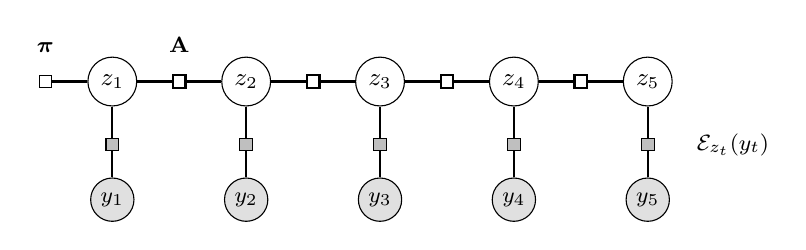
\begin{tikzpicture}[
    scale=1.0,
    state/.style={circle, draw, minimum size=0.62cm, inner sep=0.5pt, font=\small, fill=white},
    observed/.style={circle, draw, fill=black!12, minimum size=0.55cm, inner sep=0.5pt, font=\footnotesize},
    factor/.style={rectangle, draw, fill=white, minimum size=0.16cm, inner sep=0pt},
    emit/.style={rectangle, draw, fill=black!25, minimum size=0.16cm, inner sep=0pt},
    link/.style={draw, thick}
]
  \foreach \t in {1,...,5} {
    \node[state] (z\t) at (1.7*\t, 1.6) {$z_{\t}$};
    \node[emit] (e\t) at (1.7*\t, 0.8) {};
    \node[observed] (y\t) at (1.7*\t, 0.1) {$y_{\t}$};
    \draw[link] (z\t) -- (e\t) -- (y\t);
  }
  \foreach \t/\next in {1/2, 2/3, 3/4, 4/5} {
    \draw[link] (z\t) -- node[factor, pos=0.5] {} (z\next);
  }
  \node[factor] (init) at (0.85, 1.6) {};
  \draw[link] (init) -- (z1);
  \node[anchor=south, font=\footnotesize] at (0.85, 1.85) {$\bpi$};
  \node[anchor=south, font=\footnotesize] at (2.55, 1.85) {$\mathbf{A}$};
  \node[anchor=west, font=\footnotesize] at (9.0, 0.8) {$\emission_{z_t}(y_t)$};
\end{tikzpicture}
\caption{A hidden Markov model as a factor graph. Open circles are the hidden
states $z_t$ over $k$ values, open squares the transition factors
$\mathbf{A}$, the leftmost square the initial distribution $\bpi$, and shaded
squares the emission factors of the family $\emission$, each folding in one
observation $y_t$ (shaded circle). The chain is a tree, so
Equation~\ref{eq:sum-product} is exact and its two passes are
Equation~\ref{eq:forward} and Equation~\ref{eq:posterior}. Removing the
transition factors leaves the Gaussian mixture of
Section~\ref{sec:mixture}; keeping them and gating the emissions on a spatial
label gives the coupled model of Section~\ref{sec:coupled}. A sketch of the
structure and not a rendering of any instance.}
\label{fig:hmm:sketch}
\end{figure}


\paragraph{The emission family is the only part that knows what an observation
is.} Everything else---the recursions, the expectation step, path
enumeration---needs three things from it: draw an observation given a state,
score one, and re-estimate itself from posterior weights. Separating it lets
one set of recursions serve a finite alphabet, a real observation, and a count.

\paragraph{A density is not a probability.} For a family over a countable
alphabet the evidence is a probability, so $\log p(\data) \le 0$. For a family
over the reals it is a \emph{density} and carries no such bound. A check
written against the first is false under the second, so what may be asserted is
keyed on the declared support.

\subsection{The algorithm: forward--backward}
The forward recursion is Equation~\ref{eq:pruning} on a chain:
\begin{equation}
  \alpha_t(i) = \Big[ \sum_j \alpha_{t-1}(j)\, \mathbf{A}_{ji} \Big]
                \, \emission_i(y_t),
  \qquad
  p(\data) = \sum_i \alpha_T(i).
  \label{eq:forward}
\end{equation}
Pruning on a caterpillar tree carrying one observed leaf per internal node
\emph{is} this recursion \citep{durbin1998, koller2009}: the three problem
classes are one marginalization over three structures, not three unrelated
models sharing an optimizer; Appendix~\ref{app:forward-backward} derives
both passes from it. In the terms of Equation~\ref{eq:sum-product},
$\alpha_t$ is the message arriving at $z_t$ from the left multiplied by the
emission factor, the backward recursion $\beta_t$ is the same pass from the
right, and the posterior at a position is their normalized product,
\begin{equation}
  p(z_t = i \mid \data) = \frac{\alpha_t(i)\, \beta_t(i)}{p(\data)},
  \qquad
  \beta_t(i) = \sum_j \mathbf{A}_{ij}\, \emission_j(y_{t+1})\, \beta_{t+1}(j),
  \label{eq:posterior}
\end{equation}
which is the belief $b_t$ of Section~\ref{sec:notation}. Max-product on the
same chain is Viterbi,
\begin{equation}
  \delta_t(i) = \Big[\max_j\ \delta_{t-1}(j)\, \mathbf{A}_{ji}\Big]\, \emission_i(y_t),
  \label{eq:viterbi}
\end{equation}
with the path read back from the argmax at each step; on a chain with a
unique maximum the max-marginals' argmax at every position is that path
\citep{durbin1998}.

\paragraph{Regime.}
Exact for every length, the chain being a tree. The one hazard is the underflow
pruning meets, with the same remedy: the recursion runs in the logarithm.

\paragraph{What pins it.}
The sum over every one of the $k^T$ paths, written out term by term with no
recursion, referees the evidence, the posteriors and the Viterbi path at the
lengths it allows; a gradient against central differences past them. The
enumeration separates the two decoders, so no decoder can validate it; it is
pinned against algebra instead, on quantities worked out by hand on a
two-state, two-step chain.

\subsection{The algorithm: expectation-maximization}
Baum--Welch, Algorithm~\ref{alg:baum-welch}, alternates a posterior over
hidden states given the parameters with a re-estimate of the parameters given
that posterior, and increases the likelihood at every iteration
\citep{mackay2003}. The initial distribution and the transitions re-estimate in
closed form for every family; the emission re-estimate is the family's own, and
\emph{whether it is a formula} separates the families. A weighted mean is; a
dispersion parameter whose score involves the digamma function is not, and its
M step is itself an optimization---the case that says whether an interface
built around closed forms was built correctly.

\paragraph{What pins it.}
Monotonicity, asserted at every iterate; agreement of the fixed point with a
gradient fit of the same likelihood; and recovery of simulated parameters up
to the permutation of hidden states, with the alignment part of the test
(Section~\ref{sec:properties}). Where the family's M step is itself an
optimization, its refusals at the boundary of the parameter space are pinned
too: a dispersion the data cannot identify is refused, not clamped.

\subsection{Two decodings, and they are different answers}
Viterbi returns the single path of highest joint probability; posterior
decoding returns, at each position independently, the state of highest marginal
probability. Where they disagree, the posterior-decoded sequence can be a path
the model assigns zero probability to, nothing constraining consecutive choices
to be compatible. They agree on almost every instance, which is why an
implementation computing one and reporting the other survives a test suite with
no case where they diverge. Equation~\ref{eq:viterbi} and the argmax of
Equation~\ref{eq:posterior} are those two decodings; the fixture on which they
differ is constructed and kept, being the only case that tells an
implementation of one from the other. Sampling the path posterior rather than
decoding it is Algorithm~\ref{alg:chain-block}, the block sweep the coupled
model's E step also uses.

\subsection{Choosing among these at the supported sizes}
\label{sec:hmm:discussion}
Three algorithms are assumed and stated elsewhere: the two-pass
marginalization on a chain (Appendix~\ref{app:forward-backward}), the
alternation that fits it (Algorithm~\ref{alg:baum-welch}), and the block
draw of a whole path from its conditional (Algorithm~\ref{alg:chain-block}).
Unlike every other section here, none has a size at which it stops being exact:
the chain is a tree, so the recursions cost $O(T k^2)$ and are exact at every
length. The size question is therefore which referee is available, and the two
ceilings move for different reasons.

Below the path enumeration --- eleven positions at three states, seventeen at
two --- the term-by-term sum scores the evidence, both decodings and every
posterior, and it is the only thing that can, since it is what separates a
decoder computing the most probable path from one computing the per-position
modes. That is why the fixture on which the two decodings differ lives inside
this ceiling. Past it only recovery remains, and recovery needs \emph{length}
for a reason unrelated to cost: a transition matrix is identified by the number
of transitions observed, so the fixture's length is set by the variance of the
estimate and its width by the state count, while the recursion's cost stays
linear in the length.

\paragraph{Which fit, and why both are carried.}
The alternation costs one pass per iterate and increases the likelihood at
every one, so it is what to run wherever the emission family's re-estimate is a
formula. Where the re-estimate is itself an optimization --- a dispersion whose
score involves a digamma --- the guarantee is inherited only if the inner solve
converged, and an unsettled one surfaces as a non-monotone outer likelihood
several iterates later. There the gradient fit over the unconstrained vector of
Section~\ref{sec:abstraction} is the direct route. Where both apply they must
reach the same optimum, and the evidence is the agreement of two routes sharing
only the model, never the convergence of either.

\paragraph{Which decoding, and the choice is the caller's.}
The two answers are not an accuracy ordering. The most probable path minimizes
the probability of getting the whole path wrong; the per-position modes
minimize the expected number of wrong positions and may return a path the model
gives probability zero. Neither dominates, and the choice states what the
caller is scored on. Sampling the path posterior is the third answer and the
one the coupled model's expectation step needs, a decoded path being a point
estimate.

\paragraph{What the validation assumes.}
Two properties, both stated in the section and neither inherited from a
neighbouring model. The declared support decides what may be asserted at
all: over a countable alphabet the evidence is a probability and is bounded
by one, over the reals it is a density and is not, so a check written
against the first is false under the second, and it is the family's own
declaration and not the recursion that says which of the two holds. And the
parameters are identified only up to the permutation
of hidden states, so recovery carries its alignment as part of the test
rather than as a post-processing step --- an alignment chosen after seeing
the fit would referee nothing.

\subsection{Validation}
\label{sec:hmm:validation}
\begin{itemize}
  \item \emph{The sum over all $k^T$ paths}, written out term by term with no
    recursion, referees the evidence, both decodings and every posterior at the
    lengths above. It establishes the recursions exactly; separating the two
    decodings, it cannot itself be checked by a decoder, and is pinned against
    quantities worked out by hand on a two-state, two-step chain.
  \item \emph{Central differences} referee the gradient past the enumerable
    length. They establish that the differentiable path agrees with the
    recursion's own value; they establish nothing about that value.
  \item \emph{Monotonicity} referees expectation--maximization at every
    iterate. It establishes that the M step is an ascent, which is the one
    property the algorithm guarantees; it does not establish that the fixed
    point is the maximum, which is why the fixed point is also required to
    agree with an independent gradient fit of the same likelihood.
  \item \emph{Recovery up to the permutation of hidden states} is the referee
    where no oracle reaches. It establishes calibration on data from the model,
    the alignment an explicit part of the test rather than an accident of
    labelling; on a family whose M step is itself an optimization it also pins
    the boundary refusals, a dispersion the data cannot identify being refused
    and not clamped.
  \item \emph{The declared support} decides what may be asserted at all: for
    a family over a countable alphabet the evidence is a probability and
    $\log p(\data) \le 0$; for a family over the reals it is a density and
    carries no such bound. A check written against the first is false under
    the second.
\end{itemize}

\subsection{Extensions, and what is not attempted}
\label{sec:hmm:extensions}
\paragraph{What it would take to go further.}
The chain has no missing oracle inside its ceiling and none past it, so the
extensions are about the \emph{start} and the \emph{uncertainty} rather than
the recursion. A method-of-moments start would give the fit what the distance
start gives the tree: the observable moments of short windows invert to the
parameters with a consistency guarantee and no surface to climb
\citep{hsu2012}, and the argument carrying it to a tree \citep{mossel2006} is
cited in Section~\ref{sec:spectral-start}, which makes the chain the easiest
case to referee. A posterior over parameters rather than a point estimate ---
variational, or sampled by Section~\ref{sec:hmc}'s chain --- would replace the
delta-method interval whose asymptotics Section~\ref{sec:abstraction} is
explicit about \citep{bishop2006, murphy2023}. And choosing the state count
rather than declaring it is a model-selection problem this document does not
pose.

\paragraph{What is deliberately not attempted.}
Continuous time, which replaces the transition matrix by a generator and the
recursion's product by a matrix exponential --- the tree already carries that
arithmetic, and duplicating it on the chain would buy no new referee. A
semi-Markov duration model, whose state is not the position's alone, so the
factor graph is no longer the chain of Section~\ref{sec:hmm} and the path
enumeration that referees everything here does not apply. And an unbounded
state space, since every oracle in this section counts $k^T$.

\section{Problem Statement: The Coupled Spatio-Sequential Model}
\label{sec:coupled}

\subsection{The model}
\label{sec:coupled:model}
Observations $x_{sn}$ are indexed by a spatial node $n$ of a graph $\graph$ and
a sequential position $s = 1, \dots, S$. Each node carries a class label
$\ell_n \in \{1, \dots, M\}$; each class $m$ carries its own hidden chain
$k_{s,m} \in \{1, \dots, K\}$; and the observation at $(s, n)$ is emitted by
the chain of the class the node belongs to, under that class's emission
parameters $\theta_m$. The joint is Equation~\ref{eq:joint}. Its three terms
are the three problem classes above: a Potts prior on the labels,
\begin{equation}
  \log p(\ell) = \beta \sum_{\langle n,n' \rangle} J_{nn'}\,\delta(\ell_n, \ell_{n'})
                 - \log Z_{\mathrm{Potts}},
  \qquad J_{nn'} \ge 0,
  \label{eq:spatial-prior}
\end{equation}
ferromagnetic so neighbouring nodes prefer one class---the penalty on
disagreement, $-\beta \sum J_{nn'}\,\mathbb{1}[\ell_n \ne \ell_{n'}]$, is the
same distribution up to a constant; one hidden Markov chain per class, in the
simplest case with a circulant transition,
\begin{equation}
  \mathbf{A}_m(i, j) = t\,\delta_{ij} + \frac{1 - t}{K - 1}\,(1 - \delta_{ij}),
  \label{eq:circulant}
\end{equation}
whose self-transition rate $t$ and initial distribution $\Pi_m$ are fitted;
and a \emph{gated} emission, $\mathbb{1}[\ell_n = m]\,\log p(x_{sn} \mid k_{s,m},
\theta_m)$, which couples the two. Marginalizing $k$ recovers a Potts model in
a field the chains define; marginalizing $\ell$ recovers a mixture of hidden
Markov models. Neither marginal is tractable alone, and the structure of the
joint dictates the estimator.

\paragraph{Supported sizes.}
\label{par:coupled:sizes}
The joint has $M^{N} K^{SM}$ states, so the enumerable instance is small: the
canonical one is a $2 \times 2$ open lattice at $M = K = 2$ over $S = 6$
positions, $2^4 \cdot 2^{12} = 65{,}536$ joint states, inside the 200,000-state
refusal and with its emissions separated far enough that a draw at $S = 6$
identifies the classes. Past it the model runs on the lattices of
Section~\ref{sec:potts} at the sizes stated there. Under a categorical emission
the instance stays small --- a $10 \times 10$ lattice at $M = K = 2$ over four
positions --- refereed by the planted labels alone, the cell
Section~\ref{sec:applicability} marks as wanting an oracle. Under the paired
count emission of Section~\ref{sec:emissionmixture} the sequential extent
grows: an $8 \times 8$ lattice at $M = K = 2$ over 1,000 positions per pull
request, and a triangular $71 \times 71$ at $M = K = 10$ over 20,000 positions
past it. There the reference implementation of the posterior is the oracle, an
accelerated one pinned to it, and the planted labels referee the fit above
that.

\subsection{As a factor graph}
The variables are the $N$ labels and the $S M$ chain states. The factors are
the pairwise Potts factors of Section~\ref{sec:potts} on the labels, the chain
factors of Section~\ref{sec:hmm} on each class's states, and one gated
emission factor per $(n, s, m)$ over the pair $(\ell_n, k_{s,m})$, equal to
$p(x_{sn} \mid k_{s,m}, \theta_m)$ when $\ell_n = m$ and to one otherwise. A
label sits on every emission factor of its node and on every Potts factor of
its edges; in the Forney form it passes through an equality node of that
degree, and the gated factors are the higher-degree nodes joining the lattice
to the chains (Figure~\ref{fig:coupled:sketch}). That structure is for a
labelling, which Figure~\ref{fig:coupled-labelling} shows on a lattice past
enumeration, planted beside recovered. The graph has cycles, so
Equation~\ref{eq:sum-product} is the Bethe approximation on it, and the exact
quantities below come from enumeration---a $2 \times 2$ lattice with $M = 2$,
$K = 2$, $S = 3$ has $2^4 \cdot 2^{12}$ joint states.

% The Forney-style factor graph of the coupled spatio-sequential model (issue
% #290), drawn from the figure the ticket carries. Input by textbook.tex from
% sec:coupled; kept in its own file because it is a drawing and not prose.
\begin{figure}[htbp]
\centering
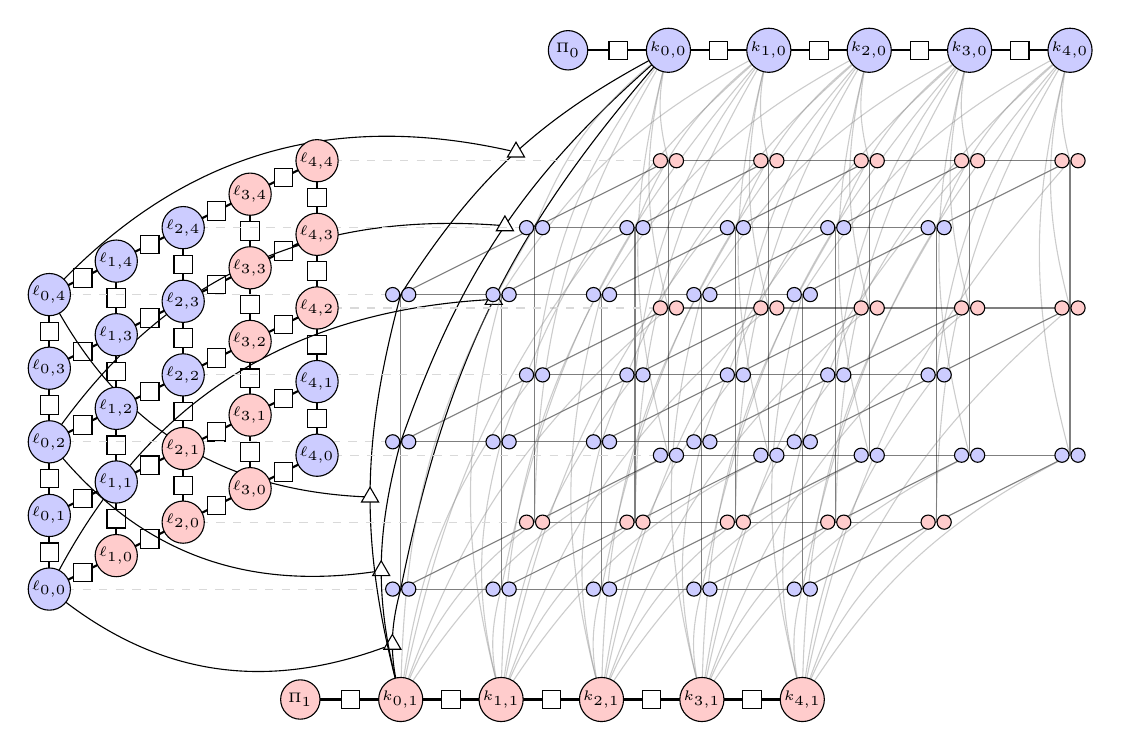
\begin{tikzpicture}[
    scale=0.85,
    x={(1.0cm, 0.5cm)},
    y={(0cm, 1.1cm)},
    z={(1.5cm, 0cm)},
    latent/.style={circle, draw, minimum size=0.50cm, inner sep=0.5pt, font=\tiny, fill=white},
    x_latent/.style={circle, draw, minimum size=0.18cm, inner sep=0pt},
    factor_style/.style={rectangle, draw, fill=white, minimum size=0.1cm},
    high_factor_style/.style={regular polygon, regular polygon sides=3, draw, fill=white, minimum size=0.25cm, inner sep=0pt},
    edge_style/.style={draw, thick, black},
    cuboid_edge/.style={draw, thin, black, opacity=0.5},
    dependency/.style={draw, thin, gray, opacity=0.4, bend left=15},
    dependency_inv/.style={draw, thin, gray, opacity=0.4, bend right=15},
    high_dep/.style={draw, thin, black, opacity=1.0},
    colorA/.style={fill=blue!20},
    colorB/.style={fill=red!20}
]
  % Lattice edges and pairwise factors
  \foreach \i in {0,...,4} {
    \foreach \j in {0,...,4} {
      \ifnum\i<4
        \draw[edge_style] (\i, \j, 0) -- (\i+1, \j, 0);
        \node[factor_style] at (\i+0.5, \j, 0) {};
      \fi
      \ifnum\j<4
        \draw[edge_style] (\i, \j, 0) -- (\i, \j+1, 0);
        \node[factor_style] at (\i, \j+0.5, 0) {};
      \fi
    }
  }
  % Markov chain edges and factors, one chain per class
  \foreach \yPos/\xPos/\chainID in {5.5/4/0, -1.5/0/1} {
    \draw[edge_style] (\xPos, \yPos, 2.5) -- (\xPos, \yPos, 3.5);
    \node[factor_style] at (\xPos, \yPos, 3.0) {};
    \foreach \k [count=\t from 0] in {3.5, 4.5, 5.5, 6.5, 7.5} {
       \ifnum\t<4
         \draw[edge_style] (\xPos, \yPos, \k) -- (\xPos, \yPos, \k+1);
         \node[factor_style] at (\xPos, \yPos, \k+0.5) {};
       \fi
    }
  }
  % Observation columns, and the gated factors joining a label to a chain state
  \foreach \i in {0,2,4} {
    \foreach \j in {0,2,4} {
      \draw[dashed, gray!30, thin] (\i, \j, 0) -- (\i, \j, 3.5);
      \foreach \k [count=\t from 0] in {3.5, 4.5, 5.5, 6.5, 7.5} {
        \ifnum\t<4 \draw[cuboid_edge] (\i, \j, \k) -- (\i, \j, \k+1); \fi
        \ifnum\i<4 \draw[cuboid_edge] (\i, \j, \k) -- (\i+2, \j, \k); \fi
        \ifnum\j<4 \draw[cuboid_edge] (\i, \j, \k) -- (\i, \j+2, \k); \fi
        \ifnum\t=0 \ifnum\i=0
            \path[high_dep, bend left=15] (\i, \j, \k) edge node[pos=0.5, high_factor_style] (f-top-\j) {} (4, 5.5, \k);
            \draw[high_dep, bend left=30] (\i, \j, 0) to (f-top-\j);
            \path[high_dep, bend right=15] (\i, \j, \k) edge node[pos=0.5, high_factor_style] (f-bot-\j) {} (0, -1.5, \k);
            \draw[high_dep, bend right=30] (\i, \j, 0) to (f-bot-\j);
        \else
            \path[dependency] (\i, \j, \k) edge (4, 5.5, \k);
            \path[dependency_inv] (\i, \j, \k) edge (0, -1.5, \k);
        \fi \else
            \path[dependency] (\i, \j, \k) edge (4, 5.5, \k);
            \path[dependency_inv] (\i, \j, \k) edge (0, -1.5, \k);
        \fi
      }
    }
  }
  % Label variables on the lattice
  \foreach \i in {0,...,4} {
    \foreach \j in {0,...,4} {
      \ifnum\i=4 \ifnum\j<2 \def\nodeCol{colorA} \else \def\nodeCol{colorB} \fi
      \else \ifnum\i>2 \def\nodeCol{colorB} \else \ifnum\j<\i \def\nodeCol{colorB} \else \def\nodeCol{colorA} \fi \fi \fi
      \node[latent, \nodeCol] at (\i, \j, 0) {$\ell_{\i,\j}$};
    }
  }
  % Chain variables
  \foreach \yPos/\xPos/\chainID in {5.5/4/0, -1.5/0/1} {
    \ifnum\chainID=0 \def\chainCol{colorA} \else \def\chainCol{colorB} \fi
    \node[latent, \chainCol] at (\xPos, \yPos, 2.5) {$\Pi_{\chainID}$};
    \foreach \k [count=\t from 0] in {3.5, 4.5, 5.5, 6.5, 7.5} {
      \node[latent, \chainCol] at (\xPos, \yPos, \k) {$k_{\t,\chainID}$};
    }
  }
  % Observations
  \foreach \i in {0,2,4} {
    \foreach \j in {0,2,4} {
      \foreach \k [count=\t from 0] in {3.5, 4.5, 5.5, 6.5, 7.5} {
        \ifnum\i=4 \ifnum\j<2 \def\xCol{colorA} \else \def\xCol{colorB} \fi
        \else \ifnum\i>2 \def\xCol{colorB} \else \ifnum\j<\i \def\xCol{colorB} \else \def\xCol{colorA} \fi \fi \fi
        \node[x_latent, \xCol] at (\i, \j, \k-0.08) {};
        \node[x_latent, \xCol] at (\i, \j, \k+0.08) {};
      }
    }
  }
\end{tikzpicture}
\caption{The coupled spatio-sequential model as a Forney-style factor graph.
Each spatial node $n$ carries a class label $\ell_n \in \{1, \dots, M\}$
(circles on the lattice, coloured by class for $M = 2$); each class $m$ carries
a hidden chain $k_{s,m} \in \{1, \dots, K\}$ with initial distribution $\Pi_m$
(the two chains at the sides). Pairwise factors (squares) carry the Potts
prior on the labels, Equation~\ref{eq:spatial-prior}, and the chain prior,
Equation~\ref{eq:circulant}. The gated emission factors (triangles) join one
label to one chain state and contribute $\log p(x_{sn} \mid k_{s,m}, \theta_m)$
only when $\ell_n = m$; the observations $x_{sn}$ are the small circles along
each column. Every second observation column is drawn along each spatial axis,
and an illustrative subset of the gated factors, so the structure is legible.}
\label{fig:coupled:sketch}
\end{figure}


\qacaptionread{figures/coupled_labelling_caption.txt}{\coupledLabellingCaption}
\begin{figure}[htbp]
  \centering
  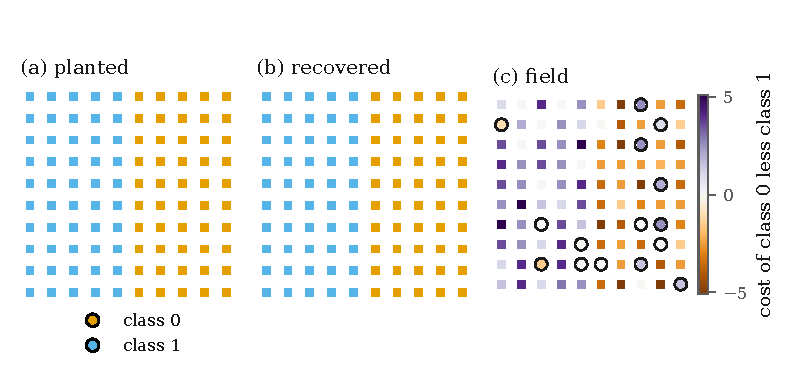
\includegraphics[width=\linewidth]{figures/coupled_labelling}
  \caption{\coupledLabellingCaption}
  \label{fig:coupled-labelling}
\end{figure}

\subsection{The estimator: block-coordinate ascent}
The blocks are the emission parameters $\theta$ and the labels $\ell$, with the
chain states marginalized. For $\theta$ given $\ell$, the gradient of the
marginal likelihood is the posterior-weighted gradient of the emission terms,
\begin{equation}
  \nabla_{\theta} \log p(x \mid \ell, \theta)
    = \sum_{n, m} \mathbb{1}[\ell_n = m] \sum_{s, k_{s,m}}
      \mathbb{Q}(k_{s,m} \mid \theta, \ell; x)\,
      \nabla_{\theta} \log p(x_{sn} \mid k_{s,m}, \theta_m),
  \label{eq:coupled-m-step}
\end{equation}
where $\mathbb{Q}$ is the per-class posterior of Equation~\ref{eq:posterior}:
this is expectation--maximization with the E step forward--backward on each
class's chain over the nodes assigned to it, and $t$ and $\Pi_m$ re-estimate
in closed form. For $\ell$ given $\theta$, the same posterior defines a
per-node, per-class external field,
\begin{equation}
  H_{nm}(\theta, \theta'; \ell) \equiv
    - \sum_{s, k_{s,m}} \mathbb{Q}(k_{s,m} \mid \theta', \ell; x)\,
      \log p(x_{sn} \mid k_{s,m}, \theta),
  \label{eq:external-field}
\end{equation}
and the label update is the ground state of a Potts model in that field,
\begin{equation}
  \ell^\star = \arg\min_{\ell}\ \beta \Big[
      \sum_{\langle n,n' \rangle} J_{nn'}\,\mathbb{1}[\ell_n \ne \ell_{n'}]
    + \sum_{n, m} \mathbb{1}[\ell_n = m]\, H_{nm} \Big],
  \label{eq:label-ground-state}
\end{equation}
which is the problem of Section~\ref{sec:alpha-expansion}, solved by
alpha expansion with its bound, descended by iterated conditional modes, or
sampled by an annealed cluster move with a field
(Section~\ref{sec:potts-sampling}). Each block does not decrease the joint
likelihood, which is the monotonicity every expectation--maximization here is
held to.

\paragraph{Why a cluster move.}
Under an effective spatial prior each class spans a contiguous region, and a
single-site move must cross it one node at a time against the prior's penalty;
iterated conditional modes freezes into spurious disjoint clusters, and
single-site annealing slows critically for the same reason. The Wolff move of
Section~\ref{sec:potts-sampling} recolours a whole cluster at once, and
Algorithm~\ref{alg:wolff-field} is that move with the field of
Equation~\ref{eq:external-field} in its accept step. At $\beta \to 0$ it is a
single-site Gibbs update, at $\beta \gg 1$ the greedy entrapment of iterated
conditional modes; annealing in $\beta$ moves between them.

\begin{algorithm}[htbp]
\caption{One Wolff update on the labels, in the external field}
\label{alg:wolff-field}
\begin{algorithmic}[1]
\State draw a root $\rho$ uniformly from the nodes; $\mu \gets \ell_\rho$;
       $\mathcal{C} \gets \{\rho\}$; queue $Q \gets \{\rho\}$
\While{$Q \ne \varnothing$}
  \State pop $n$ from $Q$
  \For{each neighbour $n'$ of $n$ with $\ell_{n'} = \mu$ and $n' \notin \mathcal{C}$}
    \State with probability $1 - e^{-\beta J_{nn'}}$: add $n'$ to $\mathcal{C}$ and to $Q$
  \EndFor
\EndWhile
\State draw a new label $\nu$ uniformly from $\{1, \dots, M\}$
\State $\Delta H \gets \sum_{n \in \mathcal{C}} (H_{n\nu} - H_{n\mu})$
\State with probability $\min\{1, e^{-\beta \Delta H}\}$: $\ell_n \gets \nu$ for every $n \in \mathcal{C}$
\end{algorithmic}
\end{algorithm}

\subsection{The initializer: data-sampled burn-in}
A start ignoring the graph and the emission family---$k$-means$++$ on the raw
observations---leaves degenerate classes and false positives the ascent then
polishes. Algorithm~\ref{alg:graph-burnin} anneals in $\beta$ from zero, so
early on the labels are nearly free and the chains and emission parameters are
fitted to what the data alone supports, the spatial prior tightening as the
classes separate. Its seeding step,
\textsc{EmissionMixture++}, is $k$-means$++$ with the emission family's own
negative log-density in place of squared Euclidean distance
\citep{arthur2007}: candidates are drawn proportionally to how badly the
current parameters explain them, constrained to the observations the current
labels and states assign to the class being seeded. The $8(\ln K + 2)$
expected-cost bound of $k$-means$++$ is a statement about squared distance and
is not inherited; what is measured instead is recovery against a uniform start
at an equal budget, over seeds, reported whether it wins or not.

\begin{algorithm}[htbp]
\caption{Data-sampled burn-in on the coupled graph}
\label{alg:graph-burnin}
\begin{algorithmic}[1]
\State $\beta \gets 0$; $H \gets 0$; $\ell_n \sim \mathrm{Uniform}\{1, \dots, M\}$ for every node
\State $\theta \gets$ \textsc{EmissionMixture++}$(\beta, K, \theta, x)$
\While{$\beta < \beta_0$}
  \State \textsc{WolffUpdate}$(\beta, \ell, J, H)$ \Comment{Algorithm~\ref{alg:wolff-field}}
  \For{each class $m$} draw the chain $k_{\cdot, m}$ by block Gibbs given $\ell$, $\theta$ \EndFor
  \For{each state $k$} $\theta_k \gets$ \textsc{EmissionMixture++}$(\beta, K, \theta, x_k, \ell)$ \Comment{state-constrained}
  \EndFor
  \State $\mathbb{Q} \gets$ forward--backward per class (Equation~\ref{eq:posterior}); M step for $\theta$, $t$, $\Pi$
  \State $H_{nm} \gets$ Equation~\ref{eq:external-field}
  \State $\beta \gets \beta + \Delta\beta$
\EndWhile
\State \Return $\ell, \theta$
\end{algorithmic}
\end{algorithm}

\paragraph{What pins it.}
The graph of Equation~\ref{eq:joint} is constructed from the three adapters
and its log-density equals the joint written out on every assignment of an
enumerable instance; the simulator's label and state marginals are held to
enumeration; the gradient identity Equation~\ref{eq:coupled-m-step} to
central differences; the joint is non-decreasing across every block for every
label solver; and label accuracy up to permutation against the planted labels
is measured at an equal budget of sweeps for each of the three solvers, so
whether a cluster move escapes what iterated conditional modes freezes into is
a measurement and not a premise---and on the planted lattice the start, not the
move, decides it.

\subsection{Choosing among these at the supported sizes}
\label{sec:coupled:discussion}
The estimator is dictated rather than chosen: neither marginal of
Equation~\ref{eq:joint} is tractable, so the blocks are what remain, and what
is chosen is the label solver and the start. Three algorithms are assumed ---
the per-class chain marginalization of Section~\ref{sec:hmm}, one of the three
label solvers of Section~\ref{sec:potts}, and the annealed start of
Algorithm~\ref{alg:graph-burnin}, whose cluster move is
Algorithm~\ref{alg:wolff-field}.

\paragraph{What each size decides.}
The enumerable instance scores the constructed graph's log-density and the
per-class posteriors against a sum, and decides nothing about the label
solvers, which are separated past it. There the planted labels are the referee
and the choice between solvers is a measurement at an equal budget of sweeps,
whose standing result is that on the planted lattice the start decides the
labelling and the move does not.

The two axes past enumeration cost differently. The sequential extent enters
the chain pass linearly and identifies the emission parameters, so more
positions buy sharper components. The node count enters the label solve, which
is not linear in it, and buys spatial resolution alone. An instance at five
thousand nodes and twenty thousand positions is two hard problems bolted
together, refereed by the planted labelling for the first and a reference
posterior for the second.

\paragraph{Which label solver, and what each needs.}
Descent needs nothing of the model and is what remains when the budget is too
small for either alternative; it freezes into disjoint clusters, a property of
a single-site move against a prior penalizing disagreement rather than a
defect. Expansion needs the pairwise term to be a metric on labels, which
$\delta$ is, and returns the factor-of-two certificate of
Equation~\ref{eq:alpha-expansion}. The cluster move needs non-negative
couplings --- which Equation~\ref{eq:spatial-prior} has by construction, so
Section~\ref{sec:frustrated}'s refusal does not bind here --- and moves a whole
region at once, at the price of being a sampler with a schedule rather than a
solver.

\paragraph{What the validation assumes.}
One structural property carries most of Section~\ref{sec:coupled:validation}:
the gated factor has degree two, joining one label to one chain state, so
conditioning on the labels leaves a set of independent chains and the
per-class two-pass recursion \emph{is} the expectation step rather than an
approximation of it. A gate over more than one chain state would leave the same
code running and the same monotonicity holding, with the expectation step no
longer the posterior. Two weaker assumptions follow: classes are identified
only up to permutation, and the planted labelling is what a correct estimator
recovers --- strictly weaker than its being the maximum of
Equation~\ref{eq:label-ground-state}.

\subsection{Validation}
\label{sec:coupled:validation}
\begin{itemize}
  \item \emph{The joint written out} on every assignment of the enumerable
    instance referees the constructed factor graph's log-density, at equality.
    It establishes that the three adapters compose into the model
    Equation~\ref{eq:joint} states; it establishes nothing about any inference
    on it.
  \item \emph{Enumeration} of the same instance referees the simulator's
    label and state marginals and the per-class posteriors. It establishes
    exactness at $2^4 \cdot 2^{12}$ states and stops there.
  \item \emph{Central differences} referee the gradient identity
    Equation~\ref{eq:coupled-m-step}. It establishes the M step's derivative,
    not the E step's posterior, which the enumeration above covers separately.
  \item \emph{Monotonicity of the joint across every block}, for each of the
    three label solvers, referees the ascent. It establishes that no block
    decreases the likelihood; it does not order the solvers, and cannot, since
    a monotone ascent to a worse fixed point is still monotone.
  \item \emph{The planted labels}, recovered up to permutation at an equal
    budget of sweeps, are the referee for the label solvers past enumeration.
    They establish which solver reaches the planted labelling on this fixture
    --- where the measurement says it is the start and not the move that
    decides it --- and they do not establish that the planted labelling is the
    maximum of Equation~\ref{eq:label-ground-state}, which is what the
    enumerated MAP labelling on the canonical instance would add.
\end{itemize}

\subsection{Extensions, and what is not attempted}
\label{sec:coupled:extensions}
\paragraph{What it would take to go further.}
Section~\ref{sec:coupled:validation} names its own gap: the planted labelling
is what a correct estimator recovers, and nothing establishes that it maximizes
Equation~\ref{eq:label-ground-state}. An enumerated maximum-posterior labelling
on the canonical instance would turn that recovery statement into an optimality
one at one size. Past it, a bound on the joint evidence would say how far a
block ascent's fixed point sits from the best available --- the mean-field
bound of Equation~\ref{eq:mean-field-bound} from below and the tree-reweighted
bound of Equation~\ref{eq:spanning-tree-bound} from above, both stated for a
lattice and neither carried on the coupled graph. Two further directions are
model rather than referee. The spatial coupling is declared and could be
fitted, making it a parameter of the same block ascent and its identifiability
a question the enumerable instance can answer. And the label update is a
discrete search over a neighbourhood with a computable improvement --- the
decision process of Section~\ref{sec:policy-gradient} --- so a learned proposal
is admissible here on the terms it is admissible for a topology.

\paragraph{What is deliberately not attempted.}
A gate over more than one chain state. The degree-two factor is what makes
conditioning on the labels leave independent chains, so a wider gate would
leave the block structure standing and the expectation step no longer the
posterior --- the failure Table~\ref{tab:referee-assumptions} records for this
row. Joint marginalization of labels and chains, which is intractable and is
the reason the estimator is blocks at all. And a spatial prior that is not
ferromagnetic: a negative coupling would put this model on the wrong side of
Section~\ref{sec:frustrated}'s refusals and remove the cluster move the
estimator relies on.

\section{Problem Statement: Large Parsimony}
\label{sec:parsimony}

\subsection{The model}
\label{sec:parsimony:model}
Parsimony is the phylogenetic criterion with no model: a topology is scored
by the fewest state changes that explain the alignment, Equation~\ref{eq:fitch}
under unit costs and Equation~\ref{eq:sankoff} under a step matrix, with no
branch lengths and no probabilities, so the score is an integer where the
likelihood is a real number. \emph{Small} parsimony scores a given tree;
\emph{large} parsimony is the search,
\begin{equation}
  \tree^{\ast} = \arg\min_{\tree} F(\tree),
  \qquad
  F(\tree) = \sum_{s=1}^{L} F_s(\tree),
  \label{eq:large-parsimony}
\end{equation}
over the $(2n-5)!!$ unrooted topologies \citep{felsenstein2004}. NP-hard in
general, and stated as the discrete half of Section~\ref{sec:phylo} with the
continuous half removed, so the same neighbourhoods and budget accounting
serve it.

\paragraph{Supported sizes.}
\label{par:parsimony:sizes}
The same sizes as Section~\ref{sec:phylo}, with the ceiling set by the same
$(2n-5)!!$ enumeration --- five and six taxa per pull request, seven at the
stress tier, eight at the release tier, where 10,395 topologies each cost one
post-order pass rather than one optimization. A candidate being that much
cheaper is the point: at an equal budget of candidates scored, the parsimony
climb reaches a neighbourhood an order of magnitude larger than the likelihood
climb, and the trade is that the criterion is the wrong one in the region
Figure~\ref{fig:parsimony-zones} names. The brute force over every labelling
of the internal nodes is $k^{\,n-2}$ per site and obeys the same 200,000-state
refusal.

\subsection{As a factor graph}
One site is the tree factor graph of Section~\ref{sec:phylo} in the
min-plus semiring (Figure~\ref{fig:parsimony:sketch}): the pairwise factor on
a branch is the cost of a change,
$0$ on agreement and $W_{ij}$ otherwise, a leaf's indicator is $0$ at its
observed state and $\infty$ elsewhere, and the root prior is constant.
Max-product with the sum replaced by a minimum and the product by a sum is
Sankoff's recursion, and under the unit matrix Fitch's set recursion carries
the same minimum. The criterion is therefore the short-branch limit of
Equation~\ref{eq:pruning}, and Equation~\ref{eq:parsimony-bound} is where
that limit re-enters the likelihood problem, as an upper bound on
$\ell^{\ast}(\tree)$ a search can rank a neighbourhood by.

% The min-plus tree of Section~\ref{sec:parsimony}, drawn by hand. Input by
% textbook.tex; a sketch and not a rendered figure, so it is outside the
% figure cache and the render cap, which govern generated output only.
\begin{figure}[htbp]
\centering
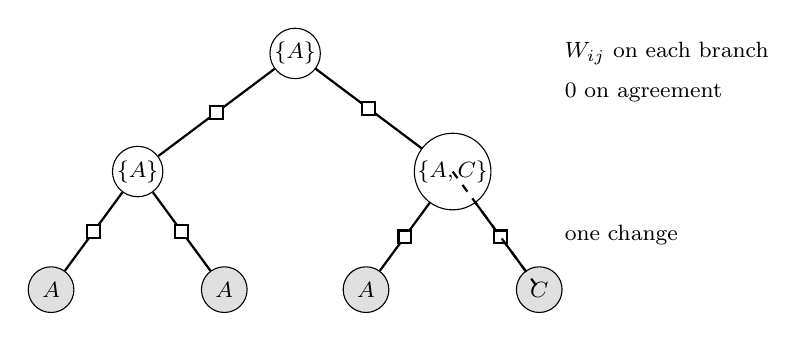
\begin{tikzpicture}[
    scale=1.0
]
  \node[fgvariable] (root) at (0, 3.4) {$\{A\}$};
  \node[fgvariable] (u)    at (-2.0, 1.9) {$\{A\}$};
  \node[fgvariable] (v)    at (2.0, 1.9) {$\{A,C\}$};
  \foreach \name/\pos/\state in {a/-3.1/A, b/-0.9/A, c/0.9/A, d/3.1/C} {
    \node[fgobserved] (\name) at (\pos, 0.4) {$\state$};
  }
  \foreach \parent/\child in {root/u, root/v, u/a, u/b, v/c, v/d} {
    \draw[fglink] (\parent) -- node[fgfactor, pos=0.5] {} (\child);
  }
  % The one change any labelling must pay, on the branch the union forces.
  \draw[thick, dashed] (2.0, 1.9) -- (3.1, 0.4);
  \node[fgnote] at (3.3, 1.1) {one change};
  \node[fgnote] at (3.3, 3.4)
    {$W_{ij}$ on each branch};
  \node[fgnote] at (3.3, 2.9)
    {$0$ on agreement};
\end{tikzpicture}
\caption{One site of large parsimony as the same tree factor graph in the
min-plus semiring. Shaded circles are the observed characters, open circles
the Fitch sets of Equation~\ref{eq:fitch} carried up the tree, and squares
the branch factors, whose table is $0$ on agreement and $W_{ij}$ otherwise
(Equation~\ref{eq:sankoff}). The right-hand cherry disagrees, so its parent
takes the union and the site's score is one change, drawn dashed on the
branch that pays it. The structure is Figure~\ref{fig:phylo:sketch} with the
probabilities replaced by costs and the branch lengths removed; the search
over the $(2n-5)!!$ topologies is what makes the problem large parsimony. A
sketch of the structure and not a rendering of any instance.}
\label{fig:parsimony:sketch}
\end{figure}


\qacaptionread{figures/parsimony_zones_caption.txt}{\parsimonyZonesCaption}
\begin{figure}[htbp]
  \centering
  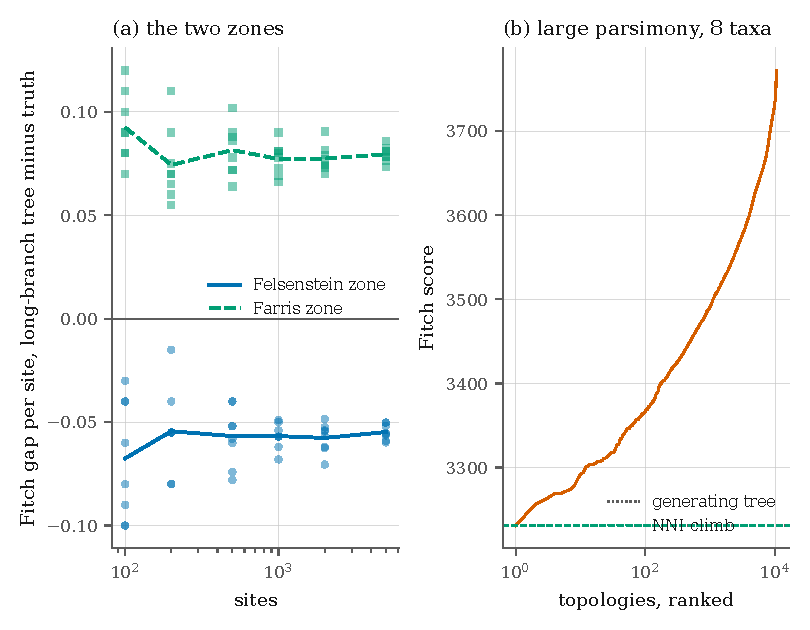
\includegraphics[width=\linewidth]{figures/parsimony_zones}
  \caption{\parsimonyZonesCaption}
  \label{fig:parsimony-zones}
\end{figure}

\subsection{The algorithm: hill climbing on the score}
The climb of Section~\ref{sec:phylo}, Algorithm~\ref{alg:hill-climbing},
with the fit replaced by one post-order pass: a random start by stepwise insertion, the best neighbour
under nearest-neighbour interchange or subtree prune-and-regraft taken while
one improves, each topology scored at most once, and the budget counted in
candidates scored. A candidate costs one pass rather than one optimization,
so the same budget reaches a neighbourhood an order of magnitude larger, and
the trade is that the criterion it climbs is the wrong one in a region that
can be named.

\paragraph{Regime.}
The step matrix must be a metric, since an unrooted topology has one score
only when every rooting scores the same; an asymmetric matrix is refused
rather than scored at an arbitrary root. And the criterion is
\emph{statistically inconsistent} in the Felsenstein zone
(Figure~\ref{fig:parsimony-zones}): with two long branches that are not a
cherry, convergent change on them is cheaper to explain by grouping them than
by the true tree, so the error rate goes to one as the alignment grows
\citep{felsenstein2004}. Moving the same branches to be a cherry gives the
Farris zone, where the criterion is consistent and fast; the pair is what
makes a measurement interpretable, because an implementation that is merely
broken fails both.

\paragraph{What pins it.}
The score against a brute force over every labelling of the internal nodes,
which shares no traversal with either recursion, at exact equality; Sankoff
under the unit matrix against Fitch on every topology of a fixture; and the
search against the enumeration of Equation~\ref{eq:large-parsimony}'s domain
from every start where it reaches, with the Felsenstein-zone fixture asserted
to return the wrong tree while the likelihood optimum on the same alignment
is the right one.

\subsection{Choosing among these at the supported sizes}
\label{sec:parsimony:discussion}
Nothing is assumed here that Section~\ref{sec:phylo} does not already
assume: the same neighbourhoods, the same budget accounting and the same
climb (Algorithm~\ref{alg:hill-climbing}), with one post-order pass in place
of one continuous optimization. The whole of the trade is that ratio, and
the whole of the objection is that the criterion it climbs is not always the
right one.

\paragraph{The trade, stated once.}
At an equal budget of candidates scored, a criterion costing one pass
reaches a neighbourhood larger than one costing a fit by the ratio of their
costs, which at the taxon counts stated above is an order of magnitude. Where the criterion is right that ratio is free
resolution, and the sensible arrangement is to \emph{search} on the score
and \emph{report} the likelihood --- which is what
Equation~\ref{eq:parsimony-bound} makes rigorous, the score entering the
likelihood problem as an upper bound a neighbourhood can be ranked by rather
than as a rival answer. Where the criterion is wrong the ratio buys nothing
at all: the Felsenstein zone is not a hard instance but a different
objective, and no budget corrects an objective. That is the reason the
criterion is carried \emph{beside} the likelihood and never instead of it.

\paragraph{What it needs of the model, and what it does not.}
It needs a step matrix that is a metric, or an unrooted topology has no
single score and the search is not well posed --- an asymmetric matrix is
refused rather than scored at an arbitrary root. It needs nothing else: no
branch lengths, no rate matrix, no stationary distribution, which is what
makes it applicable where a likelihood is not yet parameterized and why it
is the natural start for a climb that will later fit. One consequence is
easy to miss: the score is an integer, so ties are exact and frequent, where
a likelihood's ties are numerical and mean something different. A search
that breaks integer ties by the order candidates were generated is reading
its input rather than the alignment, and reports a topology that a
re-ordering would change.

\paragraph{What the validation assumes.}
The brute force over every labelling of the internal nodes referees the
score by sharing no traversal with either recursion, and it assumes only
that both are scoring the same rooted tree. The load-bearing assumption is
elsewhere: that the Felsenstein zone's inconsistency is a property of the
criterion and not of an implementation --- the strongest assumption in this
section, and the reason the zone is carried as a \emph{pair} with its
consistent counterpart: only the pair separates a defect from a theorem the
section asserts the code reproduces.

\subsection{Validation}
\label{sec:parsimony:validation}
\begin{itemize}
  \item \emph{A brute force over every labelling of the internal nodes},
    which shares no traversal with either recursion, referees the score at
    exact equality. It establishes both recursions on a given tree; it says
    nothing about the search.
  \item \emph{Fitch against Sankoff under the unit step matrix}, on every
    topology of a fixture, referees the two implementations against each
    other. It establishes that the set recursion and the cost recursion are the
    same criterion; being two of ours, it is agreement and not truth, which the
    brute force above supplies.
  \item \emph{Enumeration of Equation~\ref{eq:large-parsimony}'s domain}
    referees the climb from every start where it reaches. It establishes that
    the search found the minimum-score topology at those taxon counts.
  \item \emph{The Felsenstein-zone fixture} referees the criterion rather than
    the code: its enumerated parsimony optimum is asserted to be the wrong tree
    while the likelihood optimum on the same alignment is the right one. It
    establishes that the implementation reproduces a known statistical
    inconsistency, the one case a merely broken implementation cannot pass, and
    nothing about accuracy outside that zone, for which the Farris-zone pair is
    kept.
  \item \emph{The metric condition on the step matrix} is checked as a
    refusal, not as a result: an asymmetric matrix scores each rooting of an
    unrooted topology differently and is refused rather than scored at an
    arbitrary root.
\end{itemize}

\subsection{Extensions, and what is not attempted}
\label{sec:parsimony:extensions}
\paragraph{What it would take to go further.}
This is the one search here where an exact method past enumeration is plausibly
affordable. The score is an integer and decomposes over sites, so a partial
tree admits a lower bound on every completion and a branch and bound can
discard a whole subtree of the topology space without scoring it
\citep{papadimitriou1998, clrs2022}; a likelihood offers no such bound, which
is why an exact search would be built on the criterion first. A weighted
criterion is the other direction: the step matrix is declared here, and
estimating one from the alignment --- subject to the metric condition the
search needs --- would make the criterion a fitted model rather
than a fixed one. Compound moves are the third, and they belong to
Section~\ref{sec:policy-gradient}: a sacrifice and its payoff over this
neighbourhood are two decisions whose credit an option would carry as one
\citep{sutton1999}.

\paragraph{What is deliberately not attempted.}
A correction for the inconsistency of Figure~\ref{fig:parsimony-zones}. The
Felsenstein zone is carried as a property of the criterion and asserted
against, not repaired: the repair is the likelihood, which is
Section~\ref{sec:phylo} and already here. Ancestral-state uncertainty, since
the criterion returns a minimum and not a posterior, and the object that
carries uncertainty over internal states is the marginalization the
likelihood already does. And an asymmetric step matrix, which is refused
rather than scored at an arbitrary root.

\section{Problem Statement: Frustrated Lattices}
\label{sec:frustrated}

\subsection{The model}
\label{sec:frustrated:model}
Two instances of Equation~\ref{eq:potts} whose ground-state energy is known
from outside, admitted because more than one algorithm is scored against
them. The first is the two-state antiferromagnet, $J < 0$, on the periodic
triangular lattice: $N$ sites, $3N$ bonds, $2N$ triangles, every bond in
exactly two triangles. A triangle is not two-colourable, so each keeps at
least one agreeing bond, and counting (triangle, agreeing bond) pairs gives
$2 A \ge 2N$ for the agreeing bonds $A$ of any configuration; with a zero
field and $J = -|J|$,
\begin{equation}
  E_{\min} = |J|\, N ,
  \label{eq:triangular-ground-state}
\end{equation}
attained by many configurations: the residual entropy per site tends to
Wannier's $0.3231$ in the thermodynamic limit, a value reported for orientation
and never asserted at a finite size. The second is a planted
Viana--Bray spin glass: couplings $\pm J$ on a sparse random graph, built
around a state $\sigma^{\ast}$ by setting each coupling to reward what the
state does and then inverting a fraction $f$ of them, so that with $u$
inverted bonds
\begin{equation}
  E(\sigma^{\ast}) = -J\,\big(|E| - 2u\big),
  \qquad
  E_{\min} \le E(\sigma^{\ast}),
  \label{eq:planted-energy}
\end{equation}
a known energy at any size and an upper bound on the ground state, never the
ground state itself: at $f = 0$ the instance is a gauge transform of the
ferromagnet and trivial, and as $f$ grows the planted state stops being
near-optimal (Figure~\ref{fig:frustrated-lattices}).

\paragraph{Supported sizes.}
\label{par:frustrated:sizes}
Both instances state their answer at every size, so unlike every other
section here the size is not bounded by an oracle. The periodic triangular
lattice is carried at $3 \times 3$, $3 \times 4$, $4 \times 4$ and
$9 \times 9$; the first three are inside the $2^{|V|}$ enumeration, which
attains Equation~\ref{eq:triangular-ground-state} and measures its
degeneracy --- 42 ground states at $3 \times 3$, 68 at $3 \times 4$ and 42
again at $4 \times 4$, where neither extent divides by three --- and the
fourth is past it, where the same closed form still holds. The planted
spin glass is carried from ten to a hundred nodes at mean connectivity
three and four, with the inverted fraction $f$ swept: at $f = 0$ the instance
is a gauge transform of the ferromagnet and measures nothing, and the useful
range is where the planted state stops being near-optimal.

\subsection{As a factor graph}
The factor graph of Section~\ref{sec:potts} with $\psi_{ij} = e^{J_{ij}
\delta(\sigma_i, \sigma_j)}$ and $J_{ij} < 0$ on some or every bond. Nothing
changes in the graph; what changes is that the odd cycles of
Section~\ref{sec:potts} are now present, so the ground state is not a
colouring and the bond probability $1 - e^{-\beta J_{ij}}$ of the cluster
moves is not a probability. Figure~\ref{fig:frustrated:sketch} is the
counting argument drawn on one triangle.

% The frustrated instances of Section~\ref{sec:frustrated}, drawn by hand.
% Input by textbook.tex; a sketch and not a rendered figure, so it is outside
% the figure cache and the render cap, which govern generated output only.
\begin{figure}[htbp]
\centering
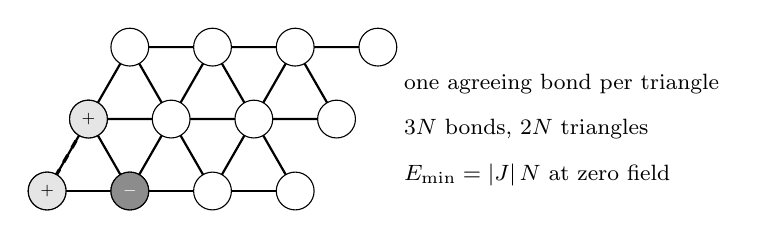
\begin{tikzpicture}[
    scale=1.05,
    % The shared vocabulary of preamble.tex. The spins are the variables of
    % Figure~\ref{fig:potts:sketch}; only the two labelled states are shaded,
    % and the lattice is drawn without its factors, the bonds standing for
    % them, because what this figure is about is the triangles.
    spin/.style={fgvariable, minimum size=0.48cm, font=\tiny},
    up/.style={spin, fill=black!10},
    down/.style={spin, fill=black!45, text=white},
    bond/.style={fglink},
    agree/.style={draw, very thick, dashed}
]
  % A patch of the triangular lattice: each row offset by half a spacing.
  \foreach \j in {0,1,2} {
    \foreach \i in {0,...,3} {
      \coordinate (n\i\j) at ({\i + 0.5*\j}, {0.87*\j});
    }
  }
  \foreach \j in {0,1,2} {
    \foreach \i in {0,1,2} {
      \draw[bond] (n\i\j) -- ({\i + 1 + 0.5*\j}, {0.87*\j});
    }
  }
  \foreach \j in {0,1} {
    \foreach \i in {0,1,2} {
      \draw[bond] (n\i\j) -- ({\i + 0.5*\j + 0.5}, {0.87*\j + 0.87});
      \draw[bond] ({\i + 1 + 0.5*\j}, {0.87*\j}) -- ({\i + 0.5*\j + 0.5}, {0.87*\j + 0.87});
    }
  }
  \foreach \j in {0,1,2} {
    \foreach \i in {0,...,3} {
      \node[spin] at (n\i\j) {};
    }
  }
  % One triangle: two spins disagree and the third bond cannot.
  \draw[agree] (n00) -- (n01);
  \node[up]   at (n00) {$+$};
  \node[down] at (n10) {$-$};
  \node[up]   at (n01) {$+$};
  \node[anchor=west, font=\footnotesize] at (4.2, 1.30)
    {one agreeing bond per triangle};
  \node[anchor=west, font=\footnotesize] at (4.2, 0.75)
    {$3N$ bonds, $2N$ triangles};
  \node[anchor=west, font=\footnotesize] at (4.2, 0.20)
    {$E_{\min} = |J|\,N$ at zero field};
\end{tikzpicture}
\caption{A patch of the periodic triangular antiferromagnet. Every bond wants
its endpoints to disagree, and a triangle is not two-colourable, so at least
one bond per triangle agrees --- the dashed bond of the labelled triangle,
where $+$ and $-$ are the two states. Counting (triangle, agreeing bond)
pairs over the $2N$ triangles and $3N$ bonds gives
Equation~\ref{eq:triangular-ground-state}, a ground-state energy known at
every size and attained by many configurations. The planted spin glass of
Equation~\ref{eq:planted-energy} is the same picture on a sparse random graph
with a fraction of the couplings inverted. A sketch of the structure and not
a rendering of any instance.}
\label{fig:frustrated:sketch}
\end{figure}


\qacaptionread{figures/frustrated_lattices_caption.txt}{\frustratedLatticesCaption}
\begin{figure}[htbp]
  \centering
  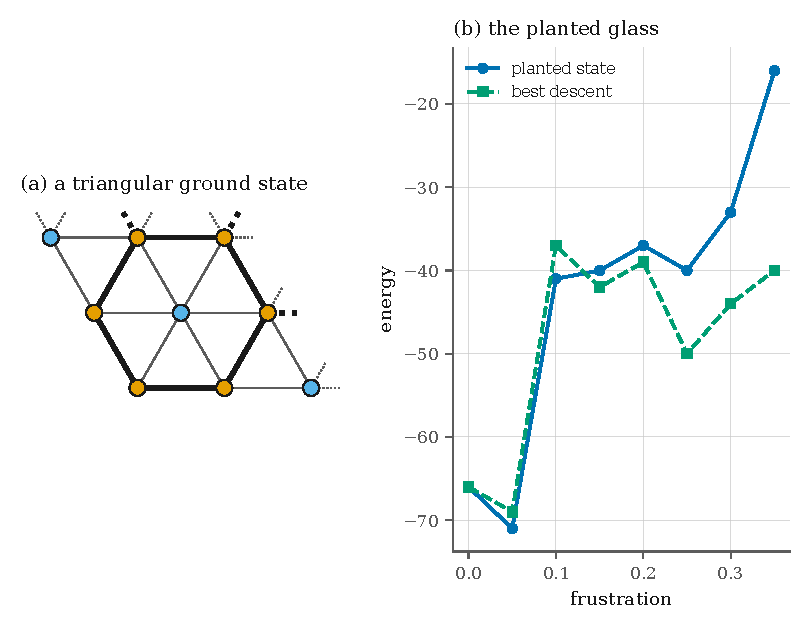
\includegraphics[width=\linewidth]{figures/frustrated_lattices}
  \caption{\frustratedLatticesCaption}
  \label{fig:frustrated-lattices}
\end{figure}

\subsection{The algorithms that apply}
Enumeration over $2^N$ configurations and the maximum cut of
Section~\ref{sec:potts-cuts}, where they reach; the semidefinite relaxation
of Equation~\ref{eq:gw}, which certifies a ratio at any size; single-site
descent, which is Algorithm~\ref{alg:heat-bath} at zero temperature, and the
annealing and parallel tempering of Section~\ref{sec:tempering},
Algorithm~\ref{alg:parallel-tempering}, which are the searches these
instances exist to separate. The exact cut refuses a negative coupling, since the energy is
not submodular, and the cluster moves refuse it for the reason above, so the
instances draw the boundary between what is solved exactly and what is only
bounded or sampled.

\subsection{The initializer}
A uniformly random configuration, and restarts of it: on a landscape whose
optimum is degenerate, which start is drawn decides which ground state is
reached and the count of restarts is part of the budget the comparison
charges.

\paragraph{What pins it.}
Equation~\ref{eq:triangular-ground-state} at every size, and enumeration
attaining it at the sizes enumeration reaches, with the degeneracy asserted
and the entropy reported; Equation~\ref{eq:planted-energy} as an inequality
on every search's result, with descent landing on the planted energy at low
$f$ and below it at high $f$ measured rather than assumed. Whether annealing
or tempering beats restarts is a property of the instance, stated as a
measurement at equal sweeps (Section~\ref{sec:tempering}).

\subsection{Choosing among these at the supported sizes}
\label{sec:frustrated:discussion}
These instances add no algorithm. Descent, annealing and replica exchange are
Section~\ref{sec:potts}'s unchanged (Algorithms~\ref{alg:heat-bath}
and~\ref{alg:parallel-tempering}); what the section supplies is an answer known
from outside at every size, so a search is scored past the reach of every other
oracle here.

\paragraph{What each instance can and cannot referee.}
The difference decides what a measurement on either may say. The triangular
antiferromagnet states an \emph{energy} and not a configuration: the optimum is
massively degenerate, so attaining
Equation~\ref{eq:triangular-ground-state} proves a search succeeded and says
nothing about which ground state it found. The planted glass states an
\emph{upper bound} and not an energy: a search returning more than
Equation~\ref{eq:planted-energy} has failed, and one reaching it has not
thereby succeeded, since at a large inverted fraction the true optimum lies
below the planted state. One instance can acquit and the other can only
convict.

\paragraph{The axis is the disorder, not the size.}
On the glass the useful parameter is the inverted fraction and not the node
count: at zero inversion the instance is a gauge transform of the ferromagnet,
a random start finds the answer and the comparison measures nothing, so the
range worth running begins where the planted state stops being near-optimal. A
success rate reported without its fraction describes no instance. On the
triangular lattice the analogous parameter is the extent, and it moves the
degeneracy rather than the energy: the closed form holds at every extent while
the number of configurations attaining it does not, which is why the extents
are declared rather than swept.

\paragraph{What is unavailable here, by construction.}
This is the one section whose applicability question is answered entirely by
refusals. The exact cut refuses, the energy not being submodular; the cluster
moves refuse, $1 - e^{-\beta J}$ not being a probability at a negative
coupling. The exact and near-exact methods are gone before the comparison
starts, and what is compared is three searches with no guarantee between any
two, at an equal budget of sweeps over shared seeds. Those refusals are checked
as results rather than described in prose.

\paragraph{What the validation assumes.}
The counting argument closes on a geometry: periodic boundaries, $3N$ bonds,
$2N$ triangles, every bond in exactly two of them. An open boundary or a
different lattice leaves the same code running and
Equation~\ref{eq:triangular-ground-state} false, and no enumeration past the
$2^{|V|}$ ceiling would notice. The residual entropy is the standing example
of a quantity reported and not asserted: it is a thermodynamic limit, and a
finite lattice is not the limit.

\subsection{Validation}
\label{sec:frustrated:validation}
\begin{itemize}
  \item \emph{Equation~\ref{eq:triangular-ground-state}}, a counting argument,
    referees the triangular ground state at every size. It establishes the
    minimum energy and that a search attaining it has attained the optimum; it
    does not identify \emph{which} ground state, the optimum being massively
    degenerate, so the residual entropy is reported for orientation and never
    asserted at a finite size.
  \item \emph{Enumeration over $2^{N}$ configurations} referees the same
    energy where it reaches, and the degeneracy with it. It establishes that
    the closed form and the code agree at the sizes both cover.
  \item \emph{Equation~\ref{eq:planted-energy}} referees every search on the
    glass as an \emph{inequality}: the planted energy is an upper bound on the
    ground state, never the ground state. It establishes that a search
    returning a higher energy has failed; it cannot establish that one
    reaching the planted energy has succeeded, and at a large inverted
    fraction a search is expected to go below it.
  \item \emph{The refusals} are checked as results: the exact cut refuses a
    negative coupling, the energy not being submodular, and the cluster moves
    refuse it because $1 - e^{-\beta J}$ is not a probability there. They
    establish that the boundary between exact and approximate is drawn in the
    code and not only in the text.
  \item \emph{An equal budget of sweeps} is what compares descent, annealing
    and tempering here. It establishes which wins \emph{on this instance}, at
    that budget, over shared seeds; it establishes nothing general about the
    algorithms, which is why the comparison is reported as an experiment.
\end{itemize}

\subsection{Extensions, and what is not attempted}
\label{sec:frustrated:extensions}
\paragraph{What it would take to go further.}
These instances are where a search is scored with no oracle, so what would
extend them is anything turning a comparison into a certificate. The
semidefinite relaxation of Equation~\ref{eq:gw} already computes one: its
optimal value bounds the maximum cut from above on the instance in hand
\citep{goemans1995, boyd2004}, so reporting it beside a search's result would
convert ``the best energy found'' into a bracket. Population annealing is the
search-side extension --- an ensemble carried down a schedule with resampling
rather than replicas exchanged along one \citep{machta2010} --- and the
comparison Section~\ref{sec:tempering} would be made against at equal sweeps. A
learned proposal is admissible on the terms
Section~\ref{sec:potts:extensions} states, and these instances, having a known
answer at every size, are where it would be measured.

\paragraph{What is deliberately not attempted.}
A disorder average. Every statement here is about one instance at one seed;
averaging over the ensemble of couplings is a different quantity needing a
different accounting, and the inverted fraction is swept so a per-instance
result is reported with the disorder it was measured at. A phase diagram, for
the reason the thermodynamic limit is out of Section~\ref{sec:potts}: the
residual entropy is quoted for orientation and asserted at no finite size. And
the exact ground state of the glass, unavailable at any size here.

\section{Problem Statement: The Gaussian Mixture}
\label{sec:mixture}

\subsection{The model}
\label{sec:mixture:model}
Independent observations $y_1, \dots, y_N$, each drawn from one of $K$
components chosen by a weight vector,
\begin{equation}
  p(y_i) = \sum_{k=1}^{K} w_k\, \mathcal{N}(y_i;\ \mu_k, \sigma_k^2),
  \qquad
  \sum_k w_k = 1,\quad w_k > 0 ,
  \label{eq:mixture}
\end{equation}
with the component label $z_i$ latent and retained by the simulator so that
a clustering has something to be checked against. It is the hidden Markov
model of Section~\ref{sec:hmm} with the chain removed: the Gaussian family is
the same emission family, and the likelihood inherits its lack of a maximum
(Section~\ref{sec:properties}) unchanged.

\paragraph{Supported sizes.}
\label{par:mixture:sizes}
$K$ components in single figures, $N$ observations from hundreds to hundreds
of thousands, and one or two channels. The simulator is checked at two
components over 200,000 draws, where a component frequency's standard error is
under 0.0011; the budgeted comparison of methods runs five components at 1.5
standard deviations of separation over 500 observations at the release tier.
\textbf{The refereed size is one-dimensional and the largest is not.} The exact
clustering cost that referees a seeding is a dynamic programme over cut
positions in the sorted observations, so it exists only on the line: in higher
dimension the same problem is NP-hard and
Equation~\ref{eq:kmeanspp-bound} would have nothing to be checked against.
A component may instead emit several channels, independent given the label, so
that a mixture matched in shape to the projection of
Section~\ref{sec:coupled} can be stated; that instance carries no oracle and
is refereed by the planted labels and the generating parameters.
Enumerating the $K^{N}$ labellings is out of reach at every size here, so the
responsibilities are refereed by the hidden Markov model's own recursion
instead.

\subsection{As a factor graph}
$N$ variables $x_i \equiv z_i$ with one unary factor each,
$\psi_i(z_i) = w_{z_i}\, \mathcal{N}(y_i; \mu_{z_i}, \sigma_{z_i}^2)$, and no
pairwise factor at all. Equation~\ref{eq:sum-product} is then a
normalization per variable, and the belief at $i$ is the responsibility
\begin{equation}
  r_{ik} = \frac{w_k\, \mathcal{N}(y_i; \mu_k, \sigma_k^2)}
                {\sum_{k'} w_{k'}\, \mathcal{N}(y_i; \mu_{k'}, \sigma_{k'}^2)} ,
  \label{eq:responsibilities}
\end{equation}
the object an HMM's forward--backward pass produces with a recursion and a
mixture with a division. The M step receiving the same object either way lets
one emission family serve both, and Figure~\ref{fig:mixture:sketch} is
Figure~\ref{fig:hmm:sketch} with the transition factors removed.

% The mixture factor graph of Section~\ref{sec:mixture}, drawn by hand. Input
% by textbook.tex; a sketch and not a rendered figure, so it is outside the
% figure cache and the render cap, which govern generated output only.
\begin{figure}[htbp]
\centering
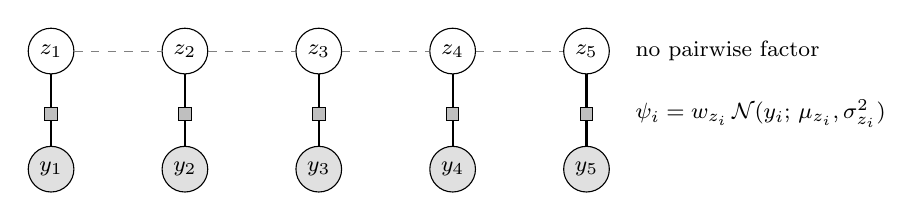
\begin{tikzpicture}[
    scale=1.0
]
  \foreach \i in {1,...,5} {
    \node[fgvariable] (z\i) at (1.7*\i, 1.6) {$z_{\i}$};
    \node[fgdata] (e\i) at (1.7*\i, 0.8) {};
    \node[fgobserved] (y\i) at (1.7*\i, 0.1) {$y_{\i}$};
    \draw[fglink] (z\i) -- (e\i) -- (y\i);
  }
  % Where the chain would be, had it not been removed.
  \foreach \i/\next in {1/2, 2/3, 3/4, 4/5} {
    \draw[fgabsent] (z\i) -- (z\next);
  }
  \node[fgnote] at (9.0, 1.6)
    {no pairwise factor};
  \node[fgnote] at (9.0, 0.8)
    {$\psi_i = w_{z_i}\,\mathcal{N}(y_i;\, \mu_{z_i}, \sigma_{z_i}^2)$};
\end{tikzpicture}
\caption{The Gaussian mixture as a factor graph: $N$ component labels $z_i$
over $K$ values, one shaded unary factor each folding in one observation
$y_i$, and no pairwise factor at all. The dashed lines mark where the
transition factors of Figure~\ref{fig:hmm:sketch} would sit; removing them is
exactly what turns the hidden Markov model into the mixture, and it turns
Equation~\ref{eq:sum-product} into the per-variable normalization that is
Equation~\ref{eq:responsibilities}. The same emission family serves both, and
receives the same responsibilities from either. A sketch of the structure and
not a rendering of any instance.}
\label{fig:mixture:sketch}
\end{figure}


\qacaptionread{figures/mixture_seeding_caption.txt}{\mixtureSeedingCaption}
\begin{figure}[htbp]
  \centering
  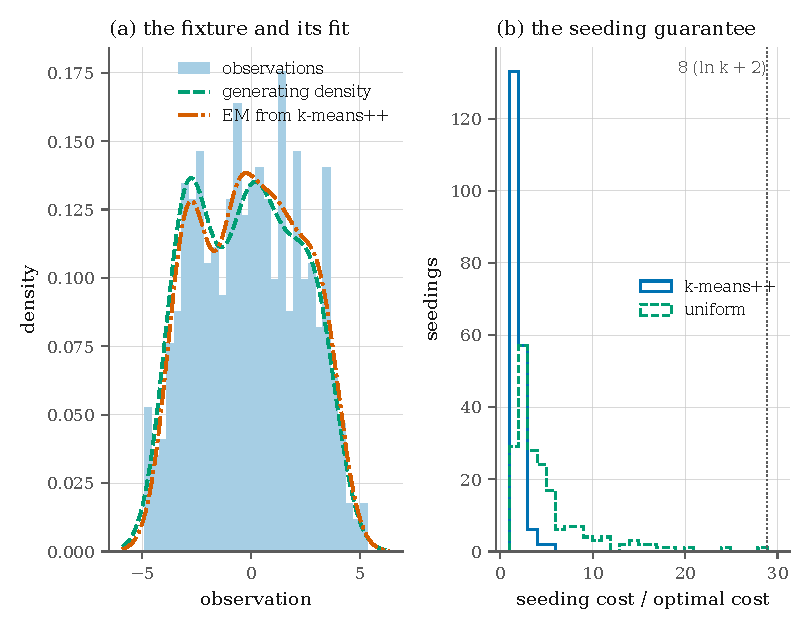
\includegraphics[width=\linewidth]{figures/mixture_seeding}
  \caption{\mixtureSeedingCaption}
  \label{fig:mixture-seeding}
\end{figure}

\subsection{The algorithms: expectation--maximization and the gradient fit}
Expectation--maximization, Algorithm~\ref{alg:baum-welch} with the chain
removed, alternates Equation~\ref{eq:responsibilities}
with the weighted re-estimate of each component's mean and variance and of
the weights as the mean responsibility, and increases the likelihood at every
iterate \citep{mackay2003}; the same objective is also fitted by the
quasi-Newton optimizer of Section~\ref{sec:abstraction} over an unconstrained
vector, the weights through a softmax and the scales through a logarithm.
The two share the model and nothing else, which makes their agreement evidence.
Where the components overlap the fixed point is approached linearly, so a raw
iterate stopped at a count sits above its basin's optimum by an amount a
gradient polish removes, and an equal-budget comparison charges the polish to
every method.

\subsection{The initializer: k-means++}
The first initializer here that reads the data, Algorithm~\ref{alg:kmeanspp}. The first centre is an
observation drawn uniformly; each subsequent one is an observation $y$ drawn
with probability proportional to its squared distance from the nearest centre
already chosen,
\begin{equation}
  \Pr(c_{j+1} = y) = \frac{D(y)^2}{\sum_{y'} D(y')^2},
  \qquad
  D(y) = \min_{j' \le j} |y - c_{j'}| ,
  \label{eq:kmeanspp}
\end{equation}
and the expected $k$-means cost of the seeding, before any refinement, is
within a factor of the optimum \citep{arthur2007}:
\begin{equation}
  \mathbb{E}\big[\,\phi(c)\,\big] \;\le\; 8\,(\ln K + 2)\; \phi^{\ast} .
  \label{eq:kmeanspp-bound}
\end{equation}
In one dimension $\phi^{\ast}$ is computable exactly---an optimal clustering
partitions the sorted observations into contiguous runs, and a dynamic
programme over the cut positions finds it---so the bound has something to be
checked against, which it does not in higher dimension where the problem is
NP-hard. Seeding is a statement about the cost and not about the likelihood:
whether a seeded start reaches a better optimum of Equation~\ref{eq:mixture}
than a uniform one is measured over seeds and reported whichever way it falls.

\paragraph{The divergence the squared distance stands for.}
Equation~\ref{eq:kmeanspp} is stated with a squared distance because the
components are isotropic Gaussians. The general rule replaces $D(y)^2$ by the
Bregman divergence of the family's log-partition \citep{banerjee2005}, which
for that family \emph{is} the squared distance over twice the variance---and
the sampling rule normalizes its scores, so a positive factor cancels and the
two are one rule. \textbf{An additive constant is not a positive factor.} The
family's negative log-density is its Bregman divergence plus the log
normalizer, and adding a constant to every score dilutes
Equation~\ref{eq:kmeanspp} toward the uniform draw in proportion to the
constant's size against a typical divergence. The two spellings are therefore
different algorithms wherever the normalizer is not small, which is a property
of the family and has to be measured per family rather than assumed.

\paragraph{What pins it.}
The component M step against the hidden Markov model's on the same
responsibilities, at equality; expectation--maximization against the
gradient fit at the same optimum, and its iterates monotone; the seeding cost
against the exact dynamic programme, with the mean over seedings held to
Equation~\ref{eq:kmeanspp-bound}; and recovery of the generating parameters
up to the permutation of components, with the alignment part of the test. A
component whose variance reaches the floor of Section~\ref{sec:properties}
is a refusal, in either algorithm.

\subsection{Choosing among these at the supported sizes}
\label{sec:mixture:discussion}
Three algorithms are assumed: the alternation of
Algorithm~\ref{alg:baum-welch} with the chain removed, the quasi-Newton fit of
Section~\ref{sec:abstraction} over the unconstrained vector, and the seeding of
Algorithm~\ref{alg:kmeanspp}. The interesting size is neither $N$ nor $K$ but
the dimension, which is one by choice.

\paragraph{Why one dimension is a decision about the referee.}
Enumerating the $K^N$ labellings is out of reach at every declared size, so the
expectation step is refereed by the chain recursion of Section~\ref{sec:hmm} on
the same responsibilities --- the one problem here whose oracle is borrowed
from a neighbouring class. The seeding's referee is the exact clustering cost,
a dynamic programme over cut positions in the sorted observations, which exists
because the observations are totally ordered. In higher dimension the same
quantity is NP-hard, so raising the dimension would not make the fit harder: it
would delete the initializer's only oracle and leave
Equation~\ref{eq:kmeanspp-bound} with nothing to check against. Growing $N$
buys precision and changes no referee.

\paragraph{Which fit.}
The alternation is cheaper per iterate and monotone; the gradient fit is
neither, and is carried because two routes sharing the model and nothing else
are evidence where one route's convergence is not. Where the components overlap
the alternation approaches its fixed point linearly, so an iterate stopped on a
count sits above its basin's optimum by an amount a polish removes --- and an
equal-budget comparison charging the polish to one method alone compares
stopping rules.

\paragraph{What the model does not have.}
There is no maximum. A component contracting onto a single observation sends
the likelihood to infinity, so what any method here finds is a local optimum by
construction, and the floor refusing such a fit is a modelling decision rather
than a numerical guard: it decides which optima are admissible. The
count-emission family of Section~\ref{sec:emissionmixture} is the same mixture
without the pathology, both channels being discrete.

\paragraph{What the validation assumes.}
Independence across observations, which makes the responsibilities a
per-observation normalization; and separation enough that ordering the
components resolves the permutation. Neither transfers: a mixture whose
components overlap past the ordering's reach fails the recovery test for a
property of the instance and not a defect of the fit, so the separation is
declared with the instance rather than discovered from it.

\subsection{Validation}
\label{sec:mixture:validation}
\begin{itemize}
  \item \emph{The hidden Markov model's M step on the same responsibilities}
    referees the mixture's, at equality. It establishes that one emission
    family serves both models; being two of ours it is agreement, not truth.
  \item \emph{The gradient fit of the same likelihood} referees
    expectation--maximization at its fixed point, and monotonicity referees
    every iterate. The two share the model and nothing else, which makes their
    agreement evidence; neither establishes that the shared optimum is global,
    and where the components overlap the fixed point is approached linearly, so
    an iterate stopped at a count sits above its basin's optimum by an amount a
    polish removes.
  \item \emph{The exact clustering cost}, a dynamic programme over the cut
    positions of the sorted observations, referees the seeding of
    Equation~\ref{eq:kmeanspp} and is the one oracle this section's
    initializer has. It establishes that the mean cost over seedings satisfies
    Equation~\ref{eq:kmeanspp-bound}; it says nothing about the likelihood,
    and whether a seeded start reaches a better optimum than a uniform one is
    measured over seeds and reported whichever way it falls.
  \item \emph{Recovery up to the permutation of components} is the referee
    for the fit itself, with the alignment part of the test. It establishes
    calibration on data from the model.
  \item \emph{The variance floor} is checked as a refusal in both algorithms:
    a component collapsing onto one observation sends the likelihood to
    infinity, so the fit refuses rather than reports it
    (Section~\ref{sec:properties}).
\end{itemize}

\subsection{Extensions, and what is not attempted}
\label{sec:mixture:extensions}
\paragraph{What it would take to go further.}
Raising the dimension costs the initializer's only oracle: the exact clustering
cost is a dynamic programme over cut positions in sorted observations and has
no counterpart above one dimension. Replacing it needs either a certified bound
on the seeding cost that does not need the optimum, or a regime where the
planted labels alone referee and the section says so ---
Section~\ref{sec:emissionmixture} already does the second at ten components.
The unbounded likelihood is the other direction: a prior on the scales, or a
penalized objective, gives a maximum that exists rather than a floor that
refuses \citep{bishop2006, murphy2023}. Choosing $K$ rather than declaring it
is model selection, and the enumerable instance is where a criterion for it
could be refereed.

\paragraph{What is deliberately not attempted.}
A component count fitted from the data, a non-diagonal covariance, and any
dimension above one --- this section exists to referee an emission family and
an initializer against exact quantities, and each of the three removes one. The
collapsing component is kept: it is the standing example of a likelihood with
no maximum, and regularizing it away would lose the case
Section~\ref{sec:properties} needs.

\section{Problem Statement: The Count-Emission Mixture}
\label{sec:emissionmixture}

\subsection{The model}
\label{sec:emissionmixture:model}
Section~\ref{sec:mixture}'s mixture with its component family exchanged, which
is the point: the mixture asks its components for a density and an M step and
nothing else, so a family over a different observation drops in unaltered. Here
the observation is a \emph{pair}---a total count
$n_i$ and the successes $y_i$ within it, a sequencing depth and its allele
count---and each component is a negative binomial for the total together with
a beta-binomial for the successes,
\begin{equation}
  p(n_i, y_i) = \sum_{k=1}^{K} w_k\,
    \mathrm{NB}(n_i;\ r_k, \mu_k)\;
    \mathrm{BB}(y_i;\ m_{ik},\ a_k, b_k),
  \qquad \sum_k w_k = 1,\quad w_k > 0 ,
  \label{eq:countpair}
\end{equation}
with the component label $z_i$ latent and retained by the simulator. The
trial count $m_{ik}$ carries the whole difference between the family's two
forms and admits no default: it is a per-component constant $m_{ik} = m_k$ in
the \emph{independent} form, where the two channels factorize given the
component, and it is the drawn total $m_{ik} = n_i$ in the \emph{joint} form,
where a deeper site carries a proportionally larger allele count. The joint
form gives $y_i > n_i$ probability zero, so a pair outside the support is
scored at $-\infty$ rather than left to the negative argument of a
$\log\Gamma$.

Two properties of Section~\ref{sec:properties} are inherited rather than
restated. The likelihood is bounded above by zero, both channels being
discrete, so the mixture has no counterpart of the Gaussian's collapsing
component. What it has instead is two \emph{flat} directions: the dispersion
$r_k$ toward the Poisson limit and the concentration $a_k + b_k$ toward the
binomial one, each with a bound above which this much data cannot tell one
value from infinity, and an estimate that reaches its bound is reported as a
bound rather than raised on.

\paragraph{Supported sizes.}
\label{par:emissionmixture:sizes}
$K$ components in single figures; $N$ observations in the hundreds to the
low thousands. The declared instances are $K = 3$ at $N = 900$, where the
posterior over labellings is enumerable, and $K = 10$, which is the size at
which the fit stops being routine. The cost per iteration is not the mixture's
but the family's: both shape parameters are solved for by bisection rather
than by formula, at a few thousand score evaluations per component per M step,
so the iteration count and not the sample count is what a budget is spent on.
Enumerating the $K^{N}$ labellings is out of reach at every declared size, and
the enumeration oracle therefore runs over a prefix: the observations are
independent, so the marginal at each of ten of them is the same quantity the
responsibilities of the whole dataset carry, and $3^{10}$ is affordable where
$3^{900}$ is not.

\subsection{As a factor graph}
$N$ variables $x_i \equiv z_i$ with one unary factor each,
$\psi_i(z_i) = w_{z_i}\, p(n_i, y_i \mid z_i)$, and no pairwise factor:
Figure~\ref{fig:emissionmixture:sketch} is
Figure~\ref{fig:mixture:sketch} with a pair at each observation instead of a
scalar. Equation~\ref{eq:sum-product} is again a normalization per variable
and the belief at $i$ is again Equation~\ref{eq:responsibilities}, now with
Equation~\ref{eq:countpair}'s density in place of the Gaussian's. That the
posterior factorizes across observations is what the enumeration oracle
checks, and it is the property every step below rests on.

% The count-emission mixture factor graph of Section~\ref{sec:emissionmixture},
% drawn by hand. Input by textbook.tex; a sketch and not a rendered figure, so
% it is outside the figure cache and the render cap, which govern generated
% output only.
\begin{figure}[htbp]
\centering
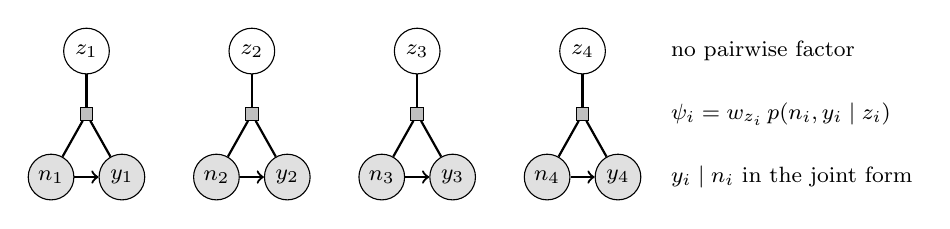
\begin{tikzpicture}[
    scale=1.0,
    within/.style={draw, thick, ->}
]
  \foreach \i in {1,...,4} {
    \node[fgvariable] (z\i) at (2.1*\i, 2.2) {$z_{\i}$};
    \node[fgdata] (e\i) at (2.1*\i, 1.4) {};
    \node[fgobserved] (n\i) at (2.1*\i - 0.45, 0.6) {$n_{\i}$};
    \node[fgobserved] (y\i) at (2.1*\i + 0.45, 0.6) {$y_{\i}$};
    \draw[fglink] (z\i) -- (e\i);
    \draw[fglink] (e\i) -- (n\i);
    \draw[fglink] (e\i) -- (y\i);
    \draw[within] (n\i) -- (y\i);
  }
  \node[fgnote] at (9.4, 2.2)
    {no pairwise factor};
  \node[fgnote] at (9.4, 1.4)
    {$\psi_i = w_{z_i}\, p(n_i, y_i \mid z_i)$};
  \node[fgnote] at (9.4, 0.6)
    {$y_i \mid n_i$ in the joint form};
\end{tikzpicture}
\caption{The count-emission mixture as a factor graph. It is
Figure~\ref{fig:mixture:sketch} with one change: the observation attached to
each unary factor is a \emph{pair}, a total $n_i$ and the successes $y_i$
within it. The arrow between them is the joint form's conditioning---the
beta-binomial's trial count is the drawn total---and is absent in the
independent form, where the trial count is a parameter and the two channels
factorize given the component. The mixture itself is unchanged either way:
Equation~\ref{eq:responsibilities} is still one normalization per variable,
and the M step is still the family's own. A sketch of the structure and not a
rendering of any instance.}
\label{fig:emissionmixture:sketch}
\end{figure}


\subsection{The algorithms: expectation--maximization and a seeded start}
Expectation--maximization, Algorithm~\ref{alg:baum-welch} with the chain
removed, exactly as for the Gaussian mixture---what differs is that the M step
it calls is itself an optimization. The negative binomial's dispersion is a
one-dimensional root find and the beta-binomial's $(a, b)$ an alternating one,
each bracketed rather than stepped toward and each reporting whether it
settled; a mixture discarding that report would surface an unsettled inner
solve several iterations later as a non-monotone outer likelihood, so it is
propagated and refused on.

The start is $\mathrm{Emission\_Mixture}{+}{+}$: Algorithm~\ref{alg:kmeanspp}
with the family's own negative log-density in place of the squared distance of
Equation~\ref{eq:kmeanspp}. A component is placed \emph{on} an observation---
its depth becomes the component's negative-binomial mean and its allele
fraction, smoothed by a half-count, the beta-binomial's rate---and the two
shape parameters, which no single observation carries, start at declared
values shared across components. The seeding is drawn over observation
\emph{indices} rather than over observation values, because a pair drawn from
a flattened array of pairs is half of one.

\paragraph{What pins it.}
The responsibilities against the posterior enumerated over component
labellings, at the size that admits one; the fitted weights and component
parameters against the planted ones, up to the permutation of components; and
the seeded start against the uniform one over shared seeds, reported whichever
way it falls.

\subsection{Choosing among these at the supported sizes}
\label{sec:emissionmixture:discussion}
Everything Section~\ref{sec:mixture} assumes is assumed here, with one
difference that moves every cost in the section: the component's
re-estimate is a bracketed solve rather than a formula
(Algorithm~\ref{alg:baum-welch}, with the family's own maximization step).
The seeding is Algorithm~\ref{alg:kmeanspp} with the family's negative
log-density in place of the squared distance, which is not a refinement but
a necessity --- a squared distance between a depth and an allele count
compares two quantities that share no units. It is the negative log-density
and not the Bregman divergence, so the caution of
Section~\ref{sec:mixture} applies: the two differ by the log normalizer, the
sampling rule does not shift its scores, and which of the two a family is
seeded under is a measurement rather than a detail.

\paragraph{The cost is the family's, not the sample's.}
Both shape parameters are found by bisection, at a few thousand score
evaluations per component per iterate, so the budget is spent on iterations and
components and barely on observations: the ten-component instance is a hard
case rather than a larger one. It also decides where a failure appears. An
inner solve that did not settle is a local event, and a mixture discarding its
report would surface it as a non-monotone outer likelihood several iterates
later, with nothing in the trace saying which component produced it --- so the
report is propagated and refused on rather than summarized.

\paragraph{Two forms, and no default between them.}
The trial count is the whole difference between the family's independent
form, in which the two channels factorize given the component, and its joint
form, in which the second channel's size is the first channel's draw. They
are different models over the same parameters: a fit under one scores
nothing about the other, and the joint form additionally puts a whole region
of the observation space at probability zero, which is a support statement
and is handled as one rather than left to a logarithm of a negative
argument.

\paragraph{What the enumeration oracle is doing.}
It runs over a prefix of ten observations, licensed by one property: the
posterior factorizes across observations, so the marginal at each of ten is the
same quantity the responsibilities of the whole dataset carry. The prefix is
therefore the test itself rather than a sample of it, and is sharpest when the
factorization is in doubt --- the property every step in this section rests on,
and the one an implementation can break without another check noticing.

\paragraph{What the validation assumes, beyond that.}
The declared form of the trial count, since the two forms are refereed by
different enumerations; and separation on depth and allele fraction sufficient
for an ordering to resolve the permutation, which a declared instance supplies
by construction and which makes an ordering admissible where enumerating the
alignments of ten components would not be. Two flat directions bound what a fit
may report: the dispersion toward the Poisson limit and the concentration
toward the binomial one each have a value above which this much data cannot
distinguish one value from infinity, so an estimate arriving there has found a
bound rather than a maximum.

\subsection{Validation}
\label{sec:emissionmixture:validation}
\begin{itemize}
  \item \emph{The enumerated posterior over component labellings} referees the
    E step at the $K = 3$ instance. An exhaustive sum sharing no code with the
    normalization it checks, it establishes that the posterior factorizes
    across observations---the property the method rests on and the one an
    implementation can quietly break. It is available over a prefix only, and
    says nothing at the $K = 10$ instance.
  \item \emph{The component M step is the emission family's own}, unchanged
    from the hidden Markov case and from the Gaussian mixture, and the family
    carries its own referees: its density sums to one over the support, and
    its estimates recover planted parameters at a stated size. Being two of
    ours it is agreement, not truth.
  \item \emph{Recovery of the planted mixture}, up to the permutation of
    components, is the referee for the fit. The permutation is resolved by
    ordering on the depth and the allele fraction rather than by enumerating
    it, since at ten components that enumeration is $10!$ and the ordering is
    exact wherever the instance separates its components---which a declared
    instance does by construction.
  \item \emph{The seeded start against the uniform one}, on the same seeds and
    the same budget, is a comparison of two of ours and establishes nothing
    general; it is reported whichever way it falls, on the terms
    Section~\ref{sec:mixture} states for $k$-means${+}{+}$.
  \item \emph{An estimate at its identifiability bound} is reported and not
    raised on: the dispersion and the concentration each have a value above
    which the data cannot distinguish the family from its limiting case, and a
    fit that reaches one has found a bound rather than a maximum
    (Section~\ref{sec:properties}).
\end{itemize}

\subsection{Extensions, and what is not attempted}
\label{sec:emissionmixture:extensions}
\paragraph{What it would take to go further.}
The flat directions are the sharpest gap. An estimate reaching its
identifiability bound is reported as a bound, and saying more needs a profile
likelihood in that direction --- the curvature being absent, the interval must
come from the objective's own shape rather than from the observed information
Section~\ref{sec:abstraction} pushes through the delta method. The M step is
the second: both shape parameters are found by bisection, and a closed form for
either would move the cost of an iterate by the factor
Section~\ref{sec:emissionmixture:discussion} says the budget is spent on. The
third is structural and built one section over: a chain over the component
labels is the coupled model of Section~\ref{sec:coupled}, so this section
carries the same family with its sequential structure removed.

\paragraph{What is deliberately not attempted.}
More than two channels, since the trial count is what ties the pair and a
third observation would need its own statement of how it is tied rather than a
default. A dispersion shared across components, which would make the flat
directions a single one and change what an identifiability bound means. And
the $K^N$ enumeration at the declared sizes: the prefix is the oracle, it
establishes the factorization and nothing else, and extending it is not
affordable at any size in this section.

\section{Problem Statement: Continuous Test Functions}
\label{sec:testfunctions}

\subsection{The functions}
\label{sec:testfunctions:model}
Three standard functions with minimizers known in closed form, so the
optimizer of Section~\ref{sec:abstraction} is checked against something that
is not a likelihood surface: on a likelihood, a fit that stops early and a
parameter the data identify weakly look the same, and these separate the
two \citep{nocedal2006}.
\begin{align}
  f_{\mathrm{R}}(x) &= \sum_{i=1}^{d-1} \Big[ b\,(x_{i+1} - x_i^2)^2 + (a - x_i)^2 \Big],
  \qquad x^{\ast} = (a, \dots, a),\ a = 1,\ b = 100,
  \label{eq:rosenbrock} \\
  f_{\mathrm{Ra}}(x) &= 10\,d + \sum_{i=1}^{d} \Big[ x_i^2 - 10 \cos(2\pi x_i) \Big],
  \qquad x^{\ast} = 0,
  \label{eq:rastrigin} \\
  f_{\mathrm{H}}(x, y) &= (x^2 + y - 11)^2 + (x + y^2 - 7)^2,
  \label{eq:himmelblau}
\end{align}
the last with four equal minima of value $0$, at $(3, 2)$ and three published
points. Rosenbrock is a curved valley whose difficulty is conditioning alone;
Rastrigin is a quadratic bowl under a cosine ripple with about $10^d$ local
minima, every one satisfying the first-order condition; Himmelblau has no
single answer, so a method that always returns the same minimum is reading its
start. They are not likelihoods: the Hessian at a minimum is not an observed
information, and no interval is built from it.
Figure~\ref{fig:testfunctions:sketch} sketches the shape of each.

% The three test surfaces of Section~\ref{sec:testfunctions}, drawn by hand.
% Input by textbook.tex; a sketch and not a rendered figure, so it is outside
% the figure cache and the render cap, which govern generated output only.
% It carries no factor graph --- the section states no model over
% variables --- so it does not use the shared vocabulary of preamble.tex;
% what is drawn is the shape of each surface.
\begin{figure}[htbp]
\centering
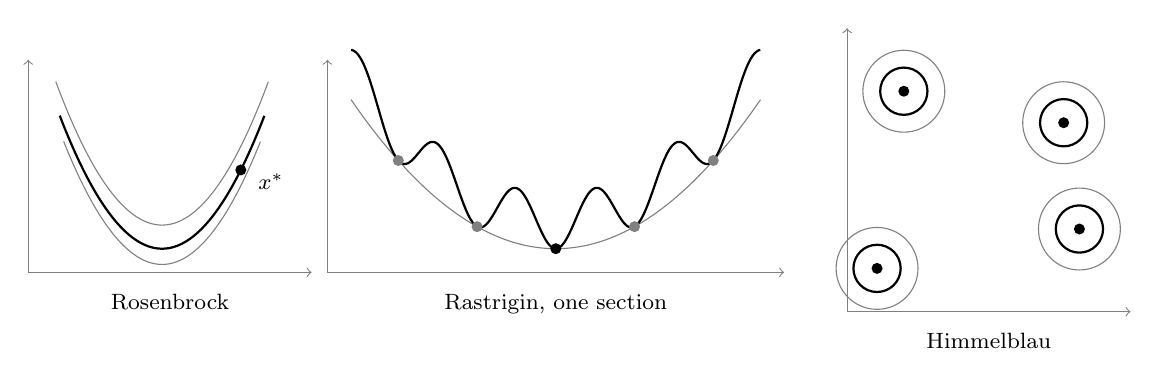
\begin{tikzpicture}[
    scale=1.0,
    curve/.style={draw, thick},
    faint/.style={draw, thin, gray},
    minimum/.style={circle, fill=black, minimum size=0.14cm, inner sep=0pt},
    axis/.style={draw, ->, thin, gray}
]
  % --- Rosenbrock: one curved valley, conditioning and nothing else -------
  \begin{scope}[xshift=0cm]
    \draw[axis] (-1.7, -0.3) -- (1.9, -0.3);
    \draw[axis] (-1.7, -0.3) -- (-1.7, 2.4);
    \draw[faint, domain=-1.35:1.35, samples=80] plot (\x, {\x*\x + 0.30});
    \draw[faint, domain=-1.25:1.25, samples=80] plot (\x, {\x*\x - 0.20});
    \draw[curve, domain=-1.3:1.3, samples=80] plot (\x, {\x*\x});
    \node[minimum] at (1.0, 1.0) {};
    \node[font=\footnotesize, anchor=west] at (1.1, 0.85) {$x^{\ast}$};
    \node[font=\footnotesize, anchor=north] at (0.1, -0.45) {Rosenbrock};
  \end{scope}
  % --- Rastrigin: a bowl under a ripple, one section of it ---------------
  \begin{scope}[xshift=5.0cm]
    \draw[axis] (-2.9, -0.3) -- (2.9, -0.3);
    \draw[axis] (-2.9, -0.3) -- (-2.9, 2.4);
    \draw[faint, domain=-2.6:2.6, samples=80] plot (\x, {0.28*\x*\x});
    \draw[curve, domain=-2.6:2.6, samples=260]
      plot (\x, {0.28*\x*\x - 0.35*cos(360*\x) + 0.35});
    \node[minimum] at (0, 0) {};
    \foreach \x in {-2,-1,1,2} { \node[minimum, fill=gray] at (\x, {0.28*\x*\x}) {}; }
    \node[font=\footnotesize, anchor=north] at (0, -0.45) {Rastrigin, one section};
  \end{scope}
  % --- Himmelblau: four basins of equal depth ----------------------------
  \begin{scope}[xshift=10.4cm, yshift=0.9cm]
    \draw[axis] (-1.7, -1.7) -- (1.9, -1.7);
    \draw[axis] (-1.7, -1.7) -- (-1.7, 1.9);
    \foreach \cx/\cy in {1.05/0.70, -0.98/1.10, -1.32/-1.15, 1.25/-0.65} {
      \draw[faint] (\cx, \cy) circle (0.52);
      \draw[curve] (\cx, \cy) circle (0.30);
      \node[minimum] at (\cx, \cy) {};
    }
    \node[font=\footnotesize, anchor=north] at (0.1, -1.85) {Himmelblau};
  \end{scope}
\end{tikzpicture}
\caption{The three surfaces, schematically. Rosenbrock is a single curved
valley whose difficulty is conditioning alone, and its minimizer is the
marked point of Equation~\ref{eq:rosenbrock}. Rastrigin, drawn as one
one-dimensional section, is a quadratic bowl under a cosine ripple: the black
point is the global minimum of Equation~\ref{eq:rastrigin} and every grey
point a local minimum satisfying the same first-order condition, of which
there are about $10^d$ in $d$ dimensions. Himmelblau has four minima of equal
value, Equation~\ref{eq:himmelblau}, so ``the'' optimum is not a well-formed
question and a method that always returns one basin is reading its start. A
sketch of the shape of each surface, not a rendering of any of them; the
rendered surfaces are Figure~\ref{fig:optimizer-landscapes}.}
\label{fig:testfunctions:sketch}
\end{figure}


\paragraph{Supported sizes.}
\label{par:testfunctions:sizes}
The size here is the dimension $d$, and it is the only problem in this
document whose oracle costs nothing at any size, the minimizers being closed
forms. Rosenbrock is fitted at $d = 2$, $3$ and $5$ and differentiated
against the closed form at $4$; Rastrigin is fitted at $d = 2$ and carried to
$3$ and $4$ by the checks that need no fit, the roughly $10^{d}$ local minima
already making a single fit's success a rate rather than an outcome;
Himmelblau is two-dimensional by definition, its four minima published
points. There is no per-tier ceiling and no enumeration: what grows with $d$ is not the cost of the referee but the
number of basins a multi-start has to find, which is why the fraction of
starts reaching the global minimum is the quantity asserted.

\qacaptionread{figures/optimizer_landscapes_caption.txt}{\optimizerLandscapesCaption}
\begin{figure}[htbp]
  \centering
  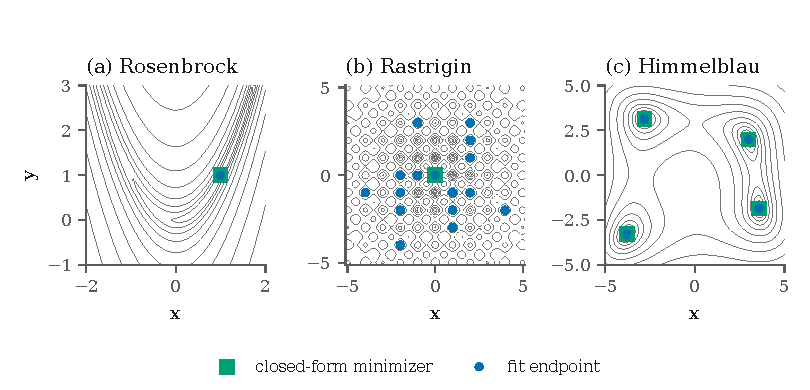
\includegraphics[width=\linewidth]{figures/optimizer_landscapes}
  \caption{\optimizerLandscapesCaption}
  \label{fig:optimizer-landscapes}
\end{figure}

\subsection{The algorithms that apply}
Each function is an instance of the objective abstraction with the identity
as its constraint map, so everything that runs on a likelihood runs on it:
the quasi-Newton fit, the Hamiltonian sampler of Section~\ref{sec:hmc} read
as an energy, and annealing with Hamiltonian proposals on a schedule
(Section~\ref{sec:tempering}). They are the continuous counterpart of the
frustrated lattices: an equal budget of objective evaluations is spent by
restarts of the fit and by an annealed chain with a polishing fit, and which
wins is a property of the surface rather than of the algorithms.

\subsection{The initializers}
The three model-free strategies, Algorithm~\ref{alg:random-restart}: the function's own start, that start tilted
by a fixed alternating amount for a surface whose nominal start is stationary,
and Gaussian restarts around it from a passed-in generator, every start
fitted and every fit reported with its spread rather than the best alone
(Figure~\ref{fig:optimizer-landscapes}). A multi-start that reports one
answer for a surface with four basins is the failure the abstraction exists
to expose.

\paragraph{What pins it.}
The fit against the analytic minimizer to a stated tolerance, in several
dimensions for Equation~\ref{eq:rosenbrock}; the automatic gradient against
the hand-written closed form, exactly; every one of Himmelblau's minima
reachable from its own basin; and on Equation~\ref{eq:rastrigin} a
\emph{rate}---the fraction of starts from which a converged fit is the global
minimum---asserted low rather than asserted to succeed, which is the
measurement that bounds what a single fit of any multimodal surface here may
claim.

\subsection{Choosing among these at the supported sizes}
\label{sec:testfunctions:discussion}
Four methods are assumed and none stated here: the quasi-Newton fit of
Section~\ref{sec:abstraction}, the Hamiltonian sampler of
Section~\ref{sec:hmc} read as an energy, annealing over that sampler on a
schedule (Section~\ref{sec:tempering}), and the restarts of
Algorithm~\ref{alg:random-restart}. The functions are carried to separate those
methods rather than to be solved, so the question is asked in reverse: which
failure does each surface expose.

\paragraph{One surface per failure.}
Conditioning alone, with a single basin: a second-order method arrives and
every global method spends its budget for nothing, so a comparison run only
on this surface reports that the cheapest local method is the best one. A
quadratic bowl under a ripple, with about $10^d$ local minima: only a method
that can cross a barrier arrives at all, restarts of a local fit convert
into a rate rather than an outcome, and a fit that stopped at a stationary
point satisfies every first-order test while being wrong. Four equal minima:
no method is right, and the failure exposed is in the \emph{reporting} --- a
multi-start that returns one answer is describing its start, and the spread
is the result. Together they are the continuous counterpart of
Section~\ref{sec:frustrated}: an equal budget of objective evaluations, and
which method wins is a property of the surface.

\paragraph{The one problem with no ceiling.}
The minimizers are closed forms, so the referee costs nothing at any dimension
and there is no per-tier size limit. What grows with $d$ is the number of
basins a multi-start must find, so the quantity that scales is a \emph{rate}
--- the fraction of starts reaching the global minimum --- asserted low rather
than asserted to succeed. That bounds what a single fit of any multimodal
surface here may claim, and it is measured here because here it can be.

\paragraph{They are not likelihoods, and that is the point.}
The Hessian at a minimum is not an observed information, so nothing here
supports an interval and the delta method of
Section~\ref{sec:abstraction} has no meaning on these surfaces. That makes
them a clean test of an optimizer and useless as a test of inference, which
is the separation they exist for: on a likelihood, a fit that stopped early
and a parameter the data identify weakly produce the same symptom, and only
a surface whose answer is known can tell the two apart.

\paragraph{What the validation assumes.}
The published minimizers, and that the automatic derivative and the
hand-written closed form are derivatives of the same function. It is the
shortest such list in this document, and the reason these functions are
carried at all.

\subsection{Validation}
\label{sec:testfunctions:validation}
\begin{itemize}
  \item \emph{The analytic minimizer} referees a fit directly, to a stated
    tolerance and in several dimensions for Equation~\ref{eq:rosenbrock}. It
    establishes that the optimizer reaches the right point on a surface where
    ``the right point'' is known --- which a likelihood cannot offer, and the
    reason these functions are carried.
  \item \emph{The hand-written closed-form gradient} referees the automatic
    one exactly. It establishes the differentiation, separately from the
    optimization, so a failure of one is not read as a failure of the other.
  \item \emph{Each of Himmelblau's four minima} is required to be reachable
    from its own basin. It establishes that the multi-start reports a spread
    rather than one answer; a method that always returns the same minimum is
    reading its start, and that is the failure this function exists to expose.
  \item \emph{A rate on Equation~\ref{eq:rastrigin}} --- the fraction of
    starts from which a converged fit is the global minimum --- is asserted
    \emph{low} rather than asserted to succeed. It establishes the bound on
    what a single fit of any multimodal surface here may claim; it establishes
    nothing about a particular run.
  \item \emph{An equal budget of objective evaluations} is what compares
    restarts against an annealed chain with a polishing fit. It establishes
    which wins on this surface at that budget, and, as with the frustrated
    lattices, nothing general about either method.
\end{itemize}

\subsection{Extensions, and what is not attempted}
\label{sec:testfunctions:extensions}
\paragraph{What it would take to go further.}
The comparison here is restarts of a local fit against an annealed chain; the
method it has not been run against is a population one, an evolution strategy
adapting a covariance from its own samples being the standard baseline for a
rugged continuous surface, scored at the same budget of objective evaluations
\citep{hansen2001}. Two reporting extensions matter more than they sound. A
rate over starts is a statistic with an interval, and stating the interval is
what makes two methods separable \citep{agarwal2021}; and the seeds, the budget
and the number of runs behind a rate are part of the claim rather than its
provenance \citep{henderson2018}. Both apply to every equal-budget comparison
here, and this is the surface where they can be checked against a known answer.

\paragraph{What is deliberately not attempted.}
Constraints, which would make the constraint map of
Section~\ref{sec:abstraction} the thing under test rather than the optimizer. A
noisy objective, since these functions are carried because their value is exact
and a fit that stopped early is distinguishable from a parameter that is not
identified. And high dimension: what grows with $d$ is the number of basins, so
a larger $d$ makes the rate smaller and the measurement no sharper.

\section{The Problems, and What Applies to Each}
\label{sec:applicability}

Tables~\ref{tab:algorithms-problems} and~\ref{tab:oracles-problems} are
generated from the problem catalogue and the regression suite, not written:
a row is a problem, a column an algorithm family or a kind of referee, and a
cell says whether the pair exists and what pins it.
Tables~\ref{tab:methods-initializers} to~\ref{tab:methods-surrogates} are the
same reading taken one method family at a time, in the grouping
Appendix~\ref{app:algorithms} uses, and add to each pairing the tier it is
validated at and a sentence on when the family wins on that problem and when it
does not --- the one hand-written part of the three, naming the experiment
where a measurement decided it. A pairing the catalogue carries and no test of
either significant kind names is marked \emph{untested} rather than omitted, so
the table cannot go quiet about a method that exists. Two readings are
load-bearing. The first is the standard: where an oracle is affordable at a
size, the method is pinned to it; where none is, recovering the simulated
truth---the generating parameters or structure of a seeded fixture, to a stated
tolerance or at a stated coverage---is sufficient, and the oracle remains
desired. The second is the marks saying where that second case holds, per
method and per size tier, so the oracle each would need is named: a
branch-and-bound bound for trees past the enumerable taxon count, a boundary
contraction for lattices past the transfer-matrix width, and for the code the
density-evolution threshold of Appendix~\ref{app:density-evolution} extended
past the erasure channel.

% Generated from PROBLEMS.md and the regression suite by the
% problems-tables generator under infra/. Do not edit; regenerate
% with its --write flag.
\begin{table}[htbp]
  \centering
  \resizebox{\textwidth}{!}{%
  \begin{tabular}{lcccccccccccc}
    \toprule
    & \rotatebox{90}{\footnotesize simulation} & \rotatebox{90}{\footnotesize exact evaluation} & \rotatebox{90}{\footnotesize message passing} & \rotatebox{90}{\footnotesize gradient fit} & \rotatebox{90}{\footnotesize expectation--maximization} & \rotatebox{90}{\footnotesize initializer} & \rotatebox{90}{\footnotesize hill climbing} & \rotatebox{90}{\footnotesize sampling and tempering} & \rotatebox{90}{\footnotesize descent and expansion} & \rotatebox{90}{\footnotesize exact ground state} & \rotatebox{90}{\footnotesize relaxation} & \rotatebox{90}{\footnotesize policy learning} \\
    \midrule
    Phylogenetic tree, Jukes--Cantor & $\checkmark$ & $\checkmark$ & -- & $\checkmark$ & -- & $\checkmark$ & $\checkmark$ & $\checkmark$ & -- & -- & -- & $\checkmark$ \\
    Phylogenetic tree, general time-reversible & $\checkmark$ & $\checkmark$ & -- & $\checkmark$ & -- & $\circ$ & $\checkmark$ & -- & -- & -- & -- & -- \\
    Phylogenetic tree, parsimony & -- & $\checkmark$ & -- & -- & -- & -- & $\checkmark$ & -- & -- & -- & -- & -- \\
    Potts chain in a field & $\checkmark$ & $\checkmark$ & -- & $\checkmark$ & -- & -- & -- & -- & -- & -- & $\checkmark$ & $\checkmark$ \\
    Potts lattice and Markov random field & $\checkmark$ & -- & $\checkmark$ & $\checkmark$ & -- & -- & -- & $\checkmark$ & $\checkmark$ & $\checkmark$ & $\checkmark$ & -- \\
    Frustrated Potts: triangular antiferromagnet, planted spin glass & $\checkmark$ & -- & -- & -- & -- & -- & -- & -- & -- & -- & -- & -- \\
    Low-density parity-check code, Gallager (3,6) & $\checkmark$ & -- & $\checkmark$ & -- & -- & -- & -- & -- & -- & -- & -- & -- \\
    Hidden Markov model, six emission families & $\checkmark$ & $\checkmark$ & -- & $\checkmark$ & $\circ$ & -- & -- & $\checkmark^{\dagger}$ & -- & -- & $\checkmark$ & $\checkmark$ \\
    Coupled spatio-sequential model & $\checkmark$ & $\checkmark$ & $\checkmark$ & -- & $\checkmark$ & $\checkmark^{\dagger}$ & -- & $\checkmark$ & -- & -- & -- & -- \\
    Gaussian mixture & $\checkmark$ & $\circ$ & -- & $\checkmark^{\dagger}$ & $\checkmark$ & $\circ$ & -- & -- & -- & -- & -- & -- \\
    Continuous test functions & -- & $\checkmark$ & -- & $\checkmark$ & -- & $\checkmark^{\dagger}$ & -- & $\checkmark$ & -- & -- & -- & -- \\
    \bottomrule
  \end{tabular}}
  \caption{The algorithms that apply to each problem, read from the problem catalogue, and what referees each: $\checkmark$ a test pinned to an oracle, $\checkmark^{\dagger}$ a test pinned to the simulated truth only, $\circ$ neither kind of test, and -- not applicable or not built. A dagger or a circle is a cell where an oracle is wanted and absent.}
  \label{tab:algorithms-problems}
\end{table}

\begin{table}[htbp]
  \centering
  \resizebox{\textwidth}{!}{%
  \begin{tabular}{lccccccc}
    \toprule
    & \rotatebox{90}{\footnotesize enumeration or brute force} & \rotatebox{90}{\footnotesize closed form or published value} & \rotatebox{90}{\footnotesize independent algorithm} & \rotatebox{90}{\footnotesize planted truth} & \rotatebox{90}{\footnotesize referee, ci tier} & \rotatebox{90}{\footnotesize referee, stress tier} & \rotatebox{90}{\footnotesize referee, release tier} \\
    \midrule
    Phylogenetic tree, Jukes--Cantor & $\checkmark$ & -- & -- & -- & oracle & -- & oracle \\
    Phylogenetic tree, general time-reversible & $\checkmark$ & -- & -- & -- & oracle & -- & truth$^{\dagger}$ \\
    Phylogenetic tree, parsimony & $\checkmark$ & -- & -- & -- & oracle & -- & oracle \\
    Potts chain in a field & $\checkmark$ & -- & -- & -- & oracle & -- & truth$^{\dagger}$ \\
    Potts lattice and Markov random field & $\checkmark$ & -- & $\checkmark$ & -- & oracle & -- & truth$^{\dagger}$ \\
    Frustrated Potts: triangular antiferromagnet, planted spin glass & -- & $\checkmark$ & -- & $\checkmark$ & oracle & -- & -- \\
    Low-density parity-check code, Gallager (3,6) & $\checkmark$ & $\checkmark$ & -- & -- & oracle & -- & truth$^{\dagger}$ \\
    Hidden Markov model, six emission families & $\checkmark$ & -- & $\checkmark$ & -- & oracle & -- & truth$^{\dagger}$ \\
    Coupled spatio-sequential model & $\checkmark$ & -- & -- & -- & oracle & -- & -- \\
    Gaussian mixture & -- & -- & $\checkmark$ & -- & oracle & -- & truth$^{\dagger}$ \\
    Continuous test functions & -- & $\checkmark$ & -- & -- & oracle & -- & truth$^{\dagger}$ \\
    \bottomrule
  \end{tabular}}
  \caption{The oracle each problem's evaluators and searches are pinned to, and, per size tier, what referees the tests that pin them: an oracle, the simulated truth only (dagger: an oracle is wanted), or no test of either kind at that tier (--). A planted truth is an upper bound on the optimum rather than the optimum.}
  \label{tab:oracles-problems}
\end{table}


\section{Problem Statement: LDPC Decoding}
\label{sec:ldpc}

\subsection{The model}
\label{sec:ldpc:model}
A binary linear code of length $n$ is the null space of a parity-check
matrix $\parity \in \{0,1\}^{m \times n}$ over $\mathrm{GF}(2)$: the
codewords are the $c$ with $\parity c = 0$, there are $2^k$ of them with
$k = n - \operatorname{rank} \parity$, and the rate is $k/n$. A
low-density code makes $\parity$ sparse. Gallager's regular
$(d_v, d_c)$ ensemble \citep{gallager1962} puts $d_v$ ones in every column
and $d_c$ in every row: $\parity$ is $d_v$ bands of $n / d_c$ rows, the
first band's row $i$ covering bits $i d_c$ to $(i+1) d_c - 1$ and every
other band the first under a uniformly random permutation of the columns,
so $n$ is a multiple of $d_c$ and $m = n d_v / d_c$. The rows of one band
sum to the all-ones vector, so at least $d_v - 1$ rows are dependent and
$k \ge n - m + d_v - 1$. The instance this repository carries is
$(3, 6)$ at $n = 19{,}998$, the multiple of six nearest the $20{,}000$ the
ticket names: $m = 9{,}999$ checks, $59{,}994$ nonzeros, design rate $1/2$.

A codeword is sent through a memoryless binary-input channel and $y$ is
received. Three channels are supported, each seen only through its
log-likelihood ratio,
\begin{equation}
  L_i = \log \frac{p(y_i \mid c_i = 0)}{p(y_i \mid c_i = 1)}
  = \begin{cases}
      (1 - 2 y_i) \log \dfrac{1 - p}{p}
        & \text{binary symmetric, flip probability } p, \\[1.2ex]
      0 \text{ if erased, else } \pm\infty \text{ with the sign of } 1 - 2 y_i
        & \text{binary erasure, erasure probability } \epsilon, \\[0.6ex]
      2 y_i / \sigma^2
        & \text{binary-input Gaussian, } y_i = (1 - 2 c_i) + \sigma z_i,
    \end{cases}
  \label{eq:ldpc-llr}
\end{equation}
positive when the received symbol favours zero. The posterior over the code
is then
\begin{equation}
  p(c \mid y) \;\propto\; \mathbb{1}[\parity c = 0]\, \exp(-c \cdot L),
  \label{eq:ldpc-code}
\end{equation}
since $\log p(y \mid c) = \sum_i \log p(y_i \mid 0) - \sum_i c_i L_i$ and the
first sum is the same for every word. Decoding asks two questions of
Equation~\ref{eq:ldpc-code}: the \emph{bitwise} MAP, each bit at the mode of
its own marginal, minimizing the bit error rate and not necessarily a codeword;
and the \emph{blockwise} MAP, the single most probable codeword, minimizing the
block error rate. They are different answers, as Section~\ref{sec:hmm} says of
the chain, and the fixture separating them is a test.

\paragraph{Supported sizes.}
\label{par:ldpc:sizes}
Codes of length $n = 12$, $24$, $48$, $96$ and $996$ carry the refereed
claims, the first being the length the codeword enumeration reaches, and
the instance the roadmap names is $(3, 6)$ at $n = 19{,}998$ with $m =
9{,}999$ checks and 59,994 nonzeros. Three ceilings separate what is refereed
by what. Enumerating the $2^{k}$ codewords is refused past 200,000 words, so
the exact decoding referee reaches $k \le 17$, which at rate $1/2$ is a code
of about 34 bits; Gauss--Jordan elimination gives a systematic encoder up to
$n = 512$, past which the all-zero codeword is sent and the argument of
Section~\ref{sec:ldpc} says nothing is lost; and past both, the referee is
the density-evolution threshold of Appendix~\ref{app:density-evolution},
which exists for the erasure channel alone. The three channels of
Equation~\ref{eq:ldpc-llr} run at every length. The bicycle construction of
Section~\ref{sec:ldpc:bicycle} is carried at $n = 12$, $96$ and $996$ with
$w = 3$, matching the first three in length and degrees, and the same three
ceilings apply to it unchanged. The quantum code of
Section~\ref{sec:ldpc:css} is carried at $n = 16$ and $96$, at $m = 7$ and
$40$ rather than $n/2$, and replaces the first of the three ceilings: its
oracle enumerates the $2^n$ errors rather than the $2^k$ codewords, so the
same 200,000 configurations reach $n = 17$.

\subsection{A second construction: bicycle codes}
\label{sec:ldpc:bicycle}
Gallager's ensemble fixes the degrees and leaves the rest to a permutation. A
bicycle code \citep{mackay2004} fixes the matrix instead. Let $A$ be the
$n/2 \times n/2$ circulant whose first row carries $w$ ones and whose row $i$
is that row shifted by $i$, and take
\begin{equation}
  \parity_0 = \begin{bmatrix} A & A^{\top} \end{bmatrix},
  \label{eq:bicycle}
\end{equation}
of shape $(n/2) \times n$. A column of the left half is a column of $A$ and a
column of the right half a row of it, and a circulant's rows and columns carry
the same weight, so every column of $\parity_0$ has weight $w$ and every row
$2w$: the $(3,6)$ degrees at $w = 3$, and a matrix determined by $w$ numbers
rather than by $d_v - 1$ permutations. Rows are then deleted to reach $m <
n/2$, which is how a rate above $1/2$ is set; \emph{which} rows is a choice,
and levelling the column weights is the one taken here, a bit in fewer checks
being the bit the decoder has least to say about.

Two properties follow from the circulant and survive any deletion. First, $A$
and $A^{\top}$ are both polynomials in the cyclic shift, so they commute and
\begin{equation}
  \parity_0 \parity_0^{\top} = A A^{\top} + A^{\top} A = 0 \pmod 2,
  \label{eq:bicycle-css}
\end{equation}
which is the condition a Calderbank--Shor--Steane quantum code puts on its two
parity-check matrices and the reason the construction was written down
\citep{mackay2004}. Nothing in the classical problem needs
Equation~\ref{eq:bicycle-css}; it is exact, and is checked as one.
Second, every row has even weight $2w$, so the all-ones word satisfies
$\parity c = 0$ and the minimum distance is at most $n$ whatever is drawn.

\paragraph{What the structure costs.}
The threshold of Appendix~\ref{app:density-evolution} is a property of the
ensemble a code is drawn from, and a bicycle code is not drawn from Gallager's:
it referees nothing here. The comparison at size is therefore against a
Gallager draw of the same length, degrees and rate on shared channel
realizations rather than against a limit, and at every setting measured the
bicycle code is the weaker of the two under the decoder of
Equation~\ref{eq:tanh-rule} --- structure paid for in cycles, and the reason
the construction is carried for what Equation~\ref{eq:bicycle-css} opens
rather than for its classical performance.

\subsection{The quantum code those matrices define}
\label{sec:ldpc:css}
Equation~\ref{eq:bicycle-css} is the condition a Calderbank--Shor--Steane code
puts on its pair of parity-check matrices, so $\parity_X = \parity_Z = \parity$
is a quantum code on $n$ qubits with
\begin{equation}
  k = n - 2 \operatorname{rank} \parity
  \label{eq:css-dimension}
\end{equation}
logical qubits \citep{mackay2004}. Everything below is one sector of it: $X$
errors against $Z$ checks, which is what a single matrix gives without a
symplectic representation of the full Pauli group.

\paragraph{The first thing to check is that there is anything to decode.}
Equation~\ref{eq:css-dimension} is zero whenever $\parity$ has full row rank
at $m = n/2$, which is the matrix Equation~\ref{eq:bicycle} gives before any
deletion. At the two lengths Section~\ref{sec:ldpc:bicycle} carries at
$m = n/2$ the rank is $m$ and $k = 0$: the code encodes nothing, every
correction is trivially right, and a measured error rate on it would be a
measurement of the zero. Deleting rows raises the rate \emph{and} the
dimension, and the instances used here have $m < n/2$ strictly.

\paragraph{What a decoder has to get right, and it is not the error.}
The stabilizer group is the row space of $\parity$; the operators commuting
with it are $\ker \parity$; and Equation~\ref{eq:bicycle-css} is exactly the
statement that the first sits inside the second. A residual
$r = e \oplus \hat e$ in the row space acts as the identity on the codespace,
so the decode \emph{succeeds} although $\hat e \neq e$; a residual in
$\ker \parity$ outside the row space is a logical operator and the decode
fails. The criterion is therefore membership of the quotient
$\ker \parity / \operatorname{rowspace} \parity$, of dimension $k$, and
agreement with the error is neither necessary nor sufficient for it. This is
\emph{degeneracy}, and it is why the referee of
Section~\ref{sec:ldpc:validation} --- the maximum-likelihood codeword --- does
not transfer: the quantity that replaces it is a coset.

\paragraph{Maximum likelihood is a sum over a coset.}
With a channel giving each error $e$ a probability $P(e)$, the decoder that
minimizes the logical error rate returns
\begin{equation}
  \hat L(s) = \operatorname*{arg\,max}_{L}
    \sum_{e \,:\, \parity e = s,\; [e] = L} P(e),
  \label{eq:coset-ml}
\end{equation}
the coset $L$ of the quotient whose members carry the most probability between
them, and not the single likeliest error. The two are different decoders, and
the second is the one a classical intuition reaches for. Summing a coset is the
optimum here, so its logical error rate is the floor any other decoder is
measured against, and the gap between the two is a property of the code rather
than of an implementation.

\paragraph{Short cycles are forced, not drawn.}
Equation~\ref{eq:bicycle-css} says every pair of rows of $\parity$ overlaps in
an even number of positions. A pair overlapping in exactly two is two checks
covering two common bits, which is a four-cycle of the Tanner graph. So the
condition that makes the quantum code exist puts short cycles into the very
graph Equation~\ref{eq:tanh-rule} needs free of them, and the count is reported
beside every decoding result rather than cited: at the enumerable instance the
graph carries thirty of them, and at the larger one a hundred and sixty.

\paragraph{Three regimes again, and the ceiling has moved.}
The oracle here enumerates \emph{errors} and not codewords, so its ceiling is
$2^n$ rather than $2^k$: the two hundred thousand configurations of
Section~\ref{sec:applicability} reach $n = 17$, where the classical oracle at
rate one-half reached about thirty-four bits. The enumerable instance therefore
carries an exact floor and a measured gap to it; past it the decoder's rate is
reported with nothing exact behind it, which the fixture states by declaring no
oracle.

\subsection{As a factor graph}
The variables are the bits, $x_i \equiv c_i \in \{0, 1\}$. The factors are a
unary $\psi_i(c_i) = e^{-c_i L_i}$ per bit, the channel folded in as an
observation is everywhere in this document, and a parity factor
$\psi_a(c_{\partial a}) = \mathbb{1}[\bigoplus_{i \in \partial a} c_i = 0]$
per row of $\parity$, a hard constraint of degree $d_c$ whose log table
is zero on even-parity assignments and $-\infty$ elsewhere. This is the
Tanner graph of the code; a bit sits on $d_v$ parity factors and one unary,
so in the Forney form every bit passes through an equality node of degree
$d_v + 1$ (Figure~\ref{fig:ldpc:sketch}). The sketch states the structure;
Figure~\ref{fig:ldpc-tanner} draws one member of the ensemble, where which bits
a check covers is the draw and not the design. The graph has cycles---a random
draw does not avoid short ones---so Equation~\ref{eq:sum-product} is the Bethe
approximation on it, and the exact quantities below come from enumerating the
$2^k$ codewords where $2^k \le 200{,}000$ (a $(3,6)$ code at $n = 24$ has
$k \ge 14$) and from the tree schedule on a cycle-free code, where message
passing is exact.

% The Tanner graph of Section~\ref{sec:ldpc}, drawn by hand. Input by
% textbook.tex; a sketch and not a rendered figure, so it is outside the
% figure cache and the render cap, which govern generated output only.
\begin{figure}[htbp]
\centering
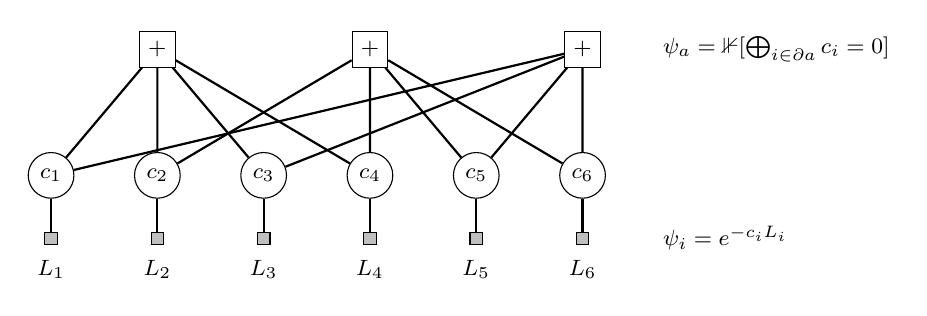
\begin{tikzpicture}[
    scale=1.0,
    check/.style={fgfactor, minimum size=0.45cm, inner sep=1pt,
                  font=\footnotesize}
]
  \foreach \i in {1,...,6} {
    \node[fgvariable] (c\i) at (1.35*\i, 1.5) {$c_{\i}$};
    \node[fgdata] (l\i) at (1.35*\i, 0.7) {};
    \draw[fglink] (c\i) -- (l\i);
    \node[font=\footnotesize, anchor=north] at (1.35*\i, 0.55) {$L_{\i}$};
  }
  \node[check] (a) at (2.7, 3.1) {$+$};
  \node[check] (b) at (5.4, 3.1) {$+$};
  \node[check] (d) at (8.1, 3.1) {$+$};
  \foreach \bit in {1,2,3,4} { \draw[fglink] (c\bit) -- (a); }
  \foreach \bit in {2,4,5,6} { \draw[fglink] (c\bit) -- (b); }
  \foreach \bit in {1,3,5,6} { \draw[fglink] (c\bit) -- (d); }
  \node[fgnote] at (9.0, 3.1)
    {$\psi_a = \mathbb{1}[\bigoplus_{i \in \partial a} c_i = 0]$};
  \node[fgnote] at (9.0, 0.7)
    {$\psi_i = e^{-c_i L_i}$};
\end{tikzpicture}
\caption{A Tanner graph: bits $c_i \in \{0, 1\}$ as circles, the parity
factors of a row of $\parity$ as squares, and the channel factor of
Equation~\ref{eq:ldpc-llr} as a shaded square carrying the log-likelihood
ratio $L_i$ at each bit. The drawn graph is six bits and three checks of
degree four; the ensemble this repository carries is regular $(3, 6)$, so
every bit sits on three parity factors and every parity factor on six bits.
The graph has cycles --- a random draw of the ensemble does not avoid short
ones --- so Equation~\ref{eq:sum-product} on it is the Bethe approximation
and Equation~\ref{eq:tanh-rule} is that approximation in the log domain. A
sketch of the structure and not a rendering of any instance.}
\label{fig:ldpc:sketch}
\end{figure}


\qacaptionread{figures/tanner_graph_caption.txt}{\tannerGraphCaption}
\begin{figure}[htbp]
  \centering
  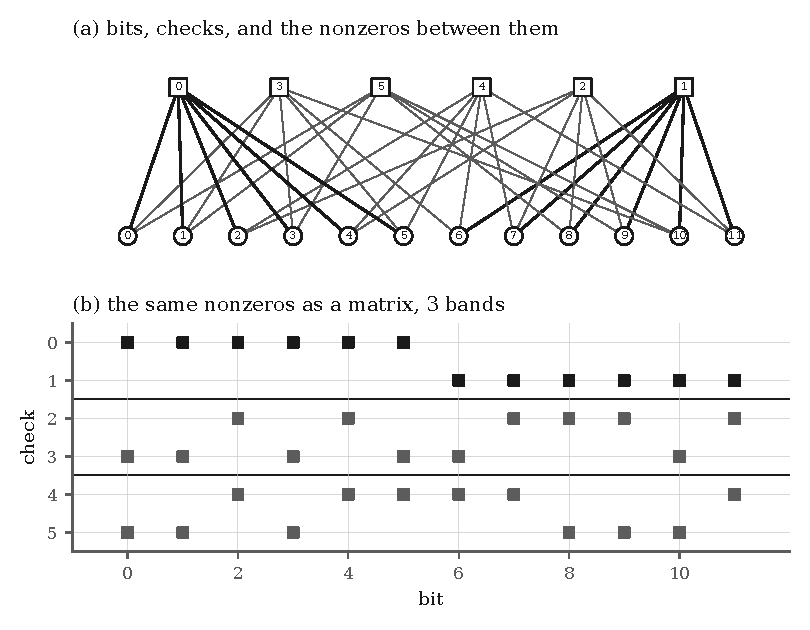
\includegraphics[width=\linewidth]{figures/tanner_graph}
  \caption{\tannerGraphCaption}
  \label{fig:ldpc-tanner}
\end{figure}

\subsection{The algorithm: sum-product in the log domain}
A binary variable's message is one number, its log-odds, and
Equation~\ref{eq:sum-product} on a parity factor has a closed form
\citep{gallager1962, mackay2003, richardson2008}; the decoder is
Algorithm~\ref{alg:sum-product-decode}. From bit $i$ to check $a$,
and from check $a$ to bit $i$,
\begin{equation}
  m_{i \to a} = L_i + \sum_{b \in \partial i \setminus a} m_{b \to i},
  \qquad
  m_{a \to i} = 2 \operatorname{artanh}
    \prod_{j \in \partial a \setminus i} \tanh \frac{m_{j \to a}}{2},
  \qquad
  \tilde L_i = L_i + \sum_{b \in \partial i} m_{b \to i},
  \label{eq:tanh-rule}
\end{equation}
where the check update follows from $\tanh(L/2) = p(0) - p(1)$ and the fact
that the parity of independent bits has a difference of probabilities equal
to the product of theirs. The hard decision $\hat c_i = \mathbb{1}[\tilde L_i
< 0]$ is the bitwise MAP under the Bethe beliefs. Replacing the sum by a
maximum in Equation~\ref{eq:sum-product} gives max-product, whose log-domain
check update is
\begin{equation}
  m_{a \to i} = \Big( \prod_{j \in \partial a \setminus i} \operatorname{sgn} m_{j \to a} \Big)
                \min_{j \in \partial a \setminus i} |m_{j \to a}|,
  \label{eq:min-sum}
\end{equation}
the min-sum decoder, whose decision is the blockwise MAP and is exact on a
cycle-free code with a unique maximum; on a loopy code it is the cheaper
and the weaker of the two, and the gap is measured rather than assumed.

Three details are load-bearing. The schedule is flooding: every check reads the
bit messages of the previous half-iteration and every bit reads the check
messages just written, one Jacobi sweep per direction over all edges at once,
the schedule the general implementation runs and so the one it is compared
against. The loop stops at
the first iteration whose hard decision has every bit decided and satisfies
$\parity \hat c = 0$, the syndrome check, and otherwise at an iteration
cap, which is a decoding failure and the event a block error rate counts. And
messages are clipped at $\pm L_{\max}$ with $L_{\max} = 30$ before the check
update, because a certain bit's ratio is infinite on the erasure channel and
the leave-one-out sums in Equation~\ref{eq:tanh-rule} are formed by
subtraction: $\tanh(L_{\max}/2)$ is below one by $1.9 \times 10^{-13}$ in
double precision, and a belief formed under the cap differs from the exact
one by less than $e^{-L_{\max}}$ in probability, which the oracle tests
absorb.

\subsection{The all-zero codeword}
Every simulation past the reach of an encoder sends the zero word, and the
argument that this loses nothing is standard \citep[Sec.~4.1]{richardson2008}.
Each channel of Equation~\ref{eq:ldpc-llr} is output symmetric: sending
$c_i = 1$ instead of $0$ negates $L_i$ in distribution, and on the symmetric
and erasure channels it negates it on every realization, since a flip or an
erasure is applied to the bit whatever its value. Both check updates are odd
in each argument and the bit update is linear, so negating the ratios at the
bits where $c_i = 1$ negates every message and every posterior at exactly
those bits, and the hard decision under $c$ is the hard decision under $0$
with $c$ added: the error pattern $c \oplus \hat c$ has the same
distribution whatever codeword was sent. Bit and block error rates measured
on the zero word are therefore the rates on any codeword. Where an encoder
exists---Gauss--Jordan elimination over $\mathrm{GF}(2)$ to a systematic
form, at $n \le 512$---the identity is checked per realization on a
non-trivial codeword, so the shortcut is itself pinned.

\paragraph{What pins it.}
Four oracles, none sharing code with the decoder. On a cycle-free code the
tree schedule of the general implementation and the enumeration over all
$2^k$ codewords are exact, and the decoder equals both; min-sum equals the
general max-product there and returns the enumerated maximum-likelihood
codeword, with the margin over the runner-up pinned so that no tie is being
broken. On loopy codes the decoder and the general damped flooding are the
same Bethe approximation and reach the same fixed point, which is agreement
and not truth. The encoder is pinned by $\parity c = 0$ and the offsets
layout by the dense product it stands in for. And at size, where no
enumeration reaches, the closed form is density evolution
(Appendix~\ref{app:density-evolution}): on the erasure channel the $(3,6)$
ensemble has a threshold $\epsilon^\star = 0.4294$ below which the
infinite-length decoder resolves every erasure and above which it does not,
and the $19{,}998$-bit code is held to bracketing it.

\subsection{Choosing among these at the supported sizes}
\label{sec:ldpc:discussion}
Four things are assumed and stated elsewhere: the specialized message
updates (Algorithm~\ref{alg:sum-product-decode}), the ensemble construction,
an elimination-based encoder, and the fixed-point recursion of
Appendix~\ref{app:density-evolution}. The choice inside the section is
between the two updates, and the choice across sizes is between three kinds
of claim that do not overlap.

\paragraph{Which update, and they answer different questions.}
The tanh rule of Equation~\ref{eq:tanh-rule} carries the whole distribution
of a check's incoming messages; the min-sum rule of
Equation~\ref{eq:min-sum} keeps a sign and a magnitude and discards the
rest. On a cycle-free code the two are the bitwise posterior and the most
probable codeword, both exact and both meaningful --- the same pair
Section~\ref{sec:hmm} draws on a chain. On a loopy code neither is exact,
and min-sum is the cheaper and the weaker; the gap between them is measured
rather than argued, and it is the reason the weaker one is kept in the
document at all.

\paragraph{Three regimes, three kinds of claim.}
Enumerating $2^k$ codewords reaches about thirty-four bits at rate
one-half, and inside that a decode is compared with an answer. To five
hundred and twelve bits an encoder exists, so a non-trivial codeword can be
transmitted and the symmetry argument that licenses everything past it is
\emph{checked} rather than assumed. Past both, the only statement is about
the ensemble rather than the code: the threshold of
Appendix~\ref{app:density-evolution} exists on the erasure channel and on
neither of the other two, so at the length the roadmap names the symmetric
and Gaussian channels carry a measured curve with no oracle behind it. That
is a marked cell in Section~\ref{sec:applicability} and not an oversight,
and what would fill it is the same recursion extended past the erasure
channel.

\paragraph{What the decoder needs of the instance.}
Sparsity, and short cycles are what cost it accuracy --- so a dense
parity-check matrix is not a small instance of this problem but a different
one, and the accuracy of a decode is a property of the graph drawn from the
ensemble rather than of the update applied to it. The message clip is the
other precondition and is a numerical one with a stated consequence: a
certain bit's ratio is infinite on the erasure channel and the leave-one-out
sums are formed by subtraction, so the clip is what makes the arithmetic
finite, and its effect on a belief is bounded in probability rather than
removed.

\paragraph{What the validation assumes.}
Output symmetry of the channel, together with the check update being odd in
each argument and the bit update linear. Those three are what make the error
pattern's distribution independent of the codeword sent, and therefore what
license every rate measured on the all-zero word past the reach of an
encoder --- which is most of the measurements in this section. The second
assumption is a stopping rule: an iteration that hits the cap is a decoding
failure and is counted as one, so a rate measured without that convention
counts a different event and is not comparable with anything here.

\subsection{Validation}
\label{sec:ldpc:validation}
\begin{itemize}
  \item \emph{Enumeration of the $2^{k}$ codewords} referees both decodings
    on a code short enough to enumerate: the bitwise posterior and the
    maximum-likelihood codeword, the latter with the margin over the runner-up
    pinned so that no tie is being broken. It establishes exactness there and
    reaches no further than the ceiling above.
  \item \emph{The tree schedule of the general sum-product} referees the
    decoder on a cycle-free code, where message passing is exact. It
    establishes that the log-domain specialization of
    Equation~\ref{eq:tanh-rule} is the same computation as the general
    implementation; on a loopy code the two agree because they are the same
    Bethe approximation, which is agreement and not truth.
  \item \emph{$\parity c = 0$ on every realization} referees the encoder, and
    the dense matrix product referees the sparse offsets layout it stands in
    for. Each establishes one construction and nothing about decoding.
  \item \emph{The channel symmetry argument} is checked rather than assumed:
    where an encoder exists, the error pattern under a non-trivial codeword is
    compared per realization with the pattern under the zero word. It
    establishes that the all-zero shortcut is sound at the lengths an encoder
    reaches, which is what licenses it past them.
  \item \emph{The erasure threshold $\epsilon^{\star} = 0.4294$} of
    Appendix~\ref{app:density-evolution} referees the 19,998-bit code, which
    is held to bracketing it. It establishes the asymptotic behaviour of the
    ensemble on one channel; it establishes nothing at finite length on the
    other two, which is the cell Section~\ref{sec:applicability} marks and the
    extension past the erasure channel would fill.
  \item \emph{The algebra of Equation~\ref{eq:bicycle}} referees the second
    construction, exactly and with no tolerance: the degrees against $w$, the
    halves against a circulant built by rolling its own first row,
    $k = n - \operatorname{rank} \parity$ against the rate each deletion
    count asks for, Equation~\ref{eq:bicycle-css} against a dense product over
    $\mathrm{GF}(2)$, and the minimum distance against an enumeration of the
    code where one reaches. It establishes what the construction is and
    nothing about how it decodes.
  \item \emph{A Gallager draw of the same length, degrees and rate} referees
    the bicycle code's decoding on shared channel realizations, and the two
    enumerated decodings bound it where they reach. It establishes where one
    construction sits against the other; it establishes nothing about either
    against the best a decoder could do at that length, which no oracle here
    reaches.
  \item \emph{The rank of $\parity$} referees the quantum code's dimension,
    Equation~\ref{eq:css-dimension}, and a basis of the quotient is built and
    checked to lie in $\ker \parity$ and outside the row space, no combination
    of it excepted. It establishes that there is a code to decode; at
    $m = n/2$ it establishes the opposite, which is why those instances carry
    no decoding claim.
  \item \emph{The criterion is refereed from both sides before a decoder runs}:
    a nonzero stabilizer added to a correct correction must read as a success
    and a logical operator must read as a failure, since an implementation
    that answers one way always passes one of the two. The membership test is
    then pinned a second way, against a label map built from a different
    computation, over every word of $\ker \parity$ at the enumerable instance.
    It establishes that the quotient is the one Equation~\ref{eq:coset-ml} is
    written in, which every number below depends on and none of which would
    visibly break if it were wrong.
  \item \emph{Enumeration of the $2^n$ errors} referees decoding under
    degeneracy: the partition carries exactly $2^k$ cosets per reachable
    syndrome and the whole probability, and Equation~\ref{eq:coset-ml} is
    evaluated on it exactly. It establishes the floor at that length and
    nothing past it, the ceiling being $n = 17$.
  \item \emph{The coset symmetry} referees the decoder being a decoder of the
    syndrome: two errors differing by a codeword are checked to give the same
    correction, which is the same argument the all-zero word rests on rather
    than a second assumption.
\end{itemize}

\subsection{Extensions, and what is not attempted}
\label{sec:ldpc:extensions}
\paragraph{What it would take to go further.}
One extension is named by the validation itself: the threshold of
Appendix~\ref{app:density-evolution} exists on the erasure channel alone, so
the symmetric and Gaussian channels have no asymptotic referee at the length
the roadmap names. Carrying the same fixed-point argument to them means
tracking a message \emph{density} rather than a single erasure probability,
either discretized or reduced to one parameter by a Gaussian approximation
\citep{richardson2008}; that is the marked cell of
Section~\ref{sec:applicability} and the single most valuable thing this
section is missing. Two further directions are the code rather than the
referee. An irregular ensemble, with a degree distribution optimized against
the threshold, is what the modern construction does and what a regular
$(3,6)$ code deliberately is not. And a decoder whose Tanner-graph edges
carry learned weights is the same message passing with the update's
parameters fitted \citep{nachmani2018}: it is admissible here because it
changes nothing about the referees --- a short code still enumerates, and a
learned decoder that beats the tanh rule on a loopy code must still equal it
on a cycle-free one.

\paragraph{What is deliberately not attempted.}
The rest of the Pauli group. Section~\ref{sec:ldpc:css} carries one CSS
sector, $X$ errors against $Z$ checks, which is what
$\parity_X = \parity_Z = \parity$ gives without a symplectic representation;
correlated $X$ and $Z$ errors --- a depolarizing channel rather than two
independent ones --- couple the two sectors, and a decoder for them decodes a
quaternary alphabet on one graph rather than a binary alphabet on two. Codes
that are not CSS are further out again: there the stabilizer generators are
not separable into two classical matrices at all, and nothing in this section
transfers unchanged. Non-binary codes, since a
binary variable's message being one number is what makes
Equation~\ref{eq:tanh-rule} a closed form rather than a sum. A channel
with memory, which breaks the per-bit factorization the unary factors rest on
and with it the symmetry argument that licenses the all-zero word. And an
encoder past the elimination's reach: past it the shortcut is used rather than
extended, and the section's job is to say what that costs, which is that the
symmetry is checked below the reach and assumed above it.

\section{Problem Statement: Turbo Decoding}
\label{sec:turbo}

\subsection{The model}
\label{sec:turbo:model}
A rate-$1/2$ \emph{recursive systematic convolutional} encoder is a linear
feedback shift register of memory $m$ over $\mathrm{GF}(2)$, stated by two
generator polynomials written in octal: a feedback $a(D)$ and a feedforward
$b(D)$, both of degree $m$ with $a_0 = b_0 = 1$. With register contents
$s_1 \dots s_m$, most recent first, one step on input $u_t$ forms the
feedback value, emits the input unchanged and one parity bit, and shifts:
\begin{equation}
  d_t = u_t \oplus \bigoplus_{i \ge 1} a_i s_i,
  \qquad
  p_t = b_0 d_t \oplus \bigoplus_{i \ge 1} b_i s_i,
  \qquad
  (s_1, \dots, s_m) \gets (d_t, s_1, \dots, s_{m-1}).
  \label{eq:rsc}
\end{equation}
The state is the register, so the encoder is a deterministic Markov chain on
$2^m$ states with two edges leaving each: a \emph{trellis}. Setting $u_t =
\bigoplus_{i \ge 1} a_i s_i$ makes $d_t = 0$, so $m$ such \emph{tail} steps
empty the register from any state --- for a recursive encoder the tail is a
function of the state and not a string of zeros, which is the whole of what
termination costs.

A \emph{turbo} code \citep{berrou1993} is two such registers fed the same
$K$-bit message in two orders. The first reads $u$; the second reads $\Pi
u$, where $\Pi$ is an interleaver, a permutation of $\{0, \dots, K-1\}$.
Both are terminated, and the transmitted word is
\begin{equation}
  c = \big(\, \underbrace{u, t^{1}}_{K + m},
              \underbrace{p^{1}}_{K + m},
              \underbrace{t^{2}}_{m},
              \underbrace{p^{2}}_{K + m} \,\big),
  \label{eq:turbo-word}
\end{equation}
with $t^{1}, t^{2}$ each encoder's tail inputs and $p^{1}, p^{2}$ its parity
stream: $n = 3K + 4m$ bits, rate $K/n$, unpunctured. The second encoder's $K$ message bits are
already carried by the first's systematic stream in a different order, which
is the whole of what the interleaver buys; its tail inputs are not, so they
are transmitted. The channel and the log-likelihood ratio convention are
Section~\ref{sec:ldpc}'s unchanged, Equation~\ref{eq:ldpc-llr}, and the
posterior over messages is Equation~\ref{eq:ldpc-code} with the code taken
as the image of the encoder.

\paragraph{Supported sizes.}
\label{par:turbo:sizes}
Message lengths $K = 12$, $256$ and $1{,}024$ carry the refereed claims, all
with the memory-2 $(7,5)$ register, so $n = 44$, $780$ and $3{,}080$. Three
ceilings separate what is refereed by what. Enumerating the $2^K$ messages
is refused past 200,000 configurations, so the exact bitwise MAP referee
reaches $K \le 17$; a dense $\mathrm{GF}(2)$ nullspace turns the code into a
parity-check matrix, and so into an instance of Section~\ref{sec:ldpc}, up
to $n = 512$; and past both the referees are the output symmetry of
Equation~\ref{eq:ldpc-llr}'s channels --- checked per realization where an
encoder is affordable --- and the uncoded closed form
$Q(\sqrt{2 E_b/N_0})$, which every coded curve must fall below at its
operating point. The convolutional decoders themselves are linear in $K$ at
every length: $2^m$ states times $K + m$ steps, with no ceiling of their
own.

\subsection{As a factor graph}
The variables of one constituent code are the $K + m + 1$ register states,
and one factor per step carries the whole of that step --- the transition
the register allows and the channel's score for the two bits it transmits:
\begin{equation}
  \psi_t(s_{t}, s_{t+1}) =
  \begin{cases}
    \exp\!\big(-u\,(L^{s}_t + L^{a}_t) - p\,L^{p}_t\big)
      & \text{if the edge } (s_t \to s_{t+1}) \text{ exists, with input } u
        \text{ and parity } p, \\
    0 & \text{otherwise,}
  \end{cases}
  \label{eq:turbo-factor}
\end{equation}
where $L^{s}, L^{p}$ are the channel ratios of the systematic and parity
bits and $L^{a}$ an a priori ratio on the input, zero for a stand-alone
decoding. The input bit needs no variable of its own: the two edges leaving
a state enter different states, so $u_t$ is recoverable from the pair. This
is a chain and the terminated boundary pins both ends, so
Equation~\ref{eq:sum-product} on the tree schedule is exact on it. That is
the difference between one constituent code and the pair. The turbo graph
joins the two chains at the message bits through $\Pi$
(Figure~\ref{fig:turbo:sketch}), which makes each message bit a variable of
degree two shared between two chains and puts a cycle around every pair of
positions the permutation reorders; no exact algorithm is available there at
the lengths the code is used at, and what is run instead is
Equation~\ref{eq:sum-product} on a serial schedule.

% The two chains and the interleaver of Section~\ref{sec:turbo}, drawn by
% hand. Input by textbook.tex; a sketch and not a rendered figure, so it is
% outside the figure cache and the render cap, which govern generated output
% only.
\begin{figure}[htbp]
\centering
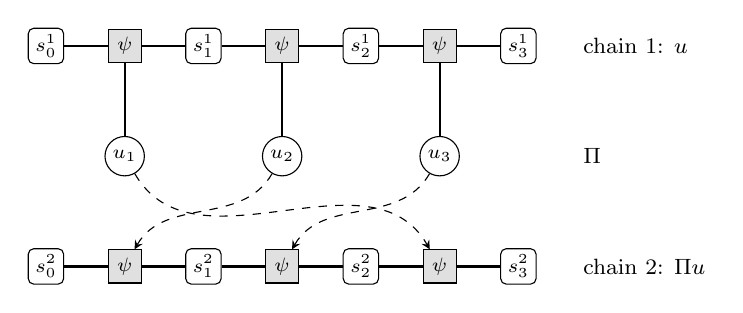
\begin{tikzpicture}[
    scale=1.0,
    bit/.style={circle, draw, minimum size=0.5cm, inner sep=0.5pt, font=\scriptsize, fill=white},
    state/.style={rectangle, draw, rounded corners=2pt, minimum size=0.45cm, inner sep=1pt, font=\scriptsize, fill=white},
    trell/.style={rectangle, draw, fill=black!12, minimum size=0.42cm, inner sep=1pt, font=\scriptsize},
    link/.style={draw, thick},
    perm/.style={draw, dashed, ->, >=stealth}
]
  % first chain
  \foreach \i/\x in {0/1.6, 1/3.6, 2/5.6, 3/7.6} {
    \node[state] (s\i) at (\x, 3.0) {$s^{1}_{\i}$};
  }
  \foreach \i/\j/\x in {0/1/2.6, 1/2/4.6, 2/3/6.6} {
    \node[trell] (t\i) at (\x, 3.0) {$\psi$};
    \draw[link] (s\i) -- (t\i); \draw[link] (t\i) -- (s\j);
  }
  \node[anchor=west, font=\footnotesize] at (8.3, 3.0) {chain 1: $u$};
  % message bits
  \foreach \i/\x in {1/2.6, 2/4.6, 3/6.6} {
    \node[bit] (u\i) at (\x, 1.6) {$u_{\i}$};
  }
  \draw[link] (t0) -- (u1);
  \draw[link] (t1) -- (u2);
  \draw[link] (t2) -- (u3);
  % second chain
  \foreach \i/\x in {0/1.6, 1/3.6, 2/5.6, 3/7.6} {
    \node[state] (r\i) at (\x, 0.2) {$s^{2}_{\i}$};
  }
  \foreach \i/\j/\x in {0/1/2.6, 1/2/4.6, 2/3/6.6} {
    \node[trell] (v\i) at (\x, 0.2) {$\psi$};
    \draw[link] (r\i) -- (v\i); \draw[link] (v\i) -- (r\j);
  }
  \node[anchor=west, font=\footnotesize] at (8.3, 0.2) {chain 2: $\Pi u$};
  \draw[perm] (u1) to[out=-60, in=120] (v2);
  \draw[perm] (u2) to[out=-120, in=60] (v0);
  \draw[perm] (u3) to[out=-120, in=60] (v1);
  \node[anchor=west, font=\footnotesize] at (8.3, 1.6) {$\Pi$};
\end{tikzpicture}
\caption{A turbo code as a factor graph: two trellis chains sharing the
message bits through a permutation. Each $\psi$ is one trellis factor of
Equation~\ref{eq:turbo-factor}, carrying both the transition the register
allows and the channel's score for the two bits that transition transmits;
each $s^{c}_{t}$ is a register state. The message bit $u_i$ is read by the
first chain at position $i$ and by the second at position $\Pi^{-1}(i)$, so
every $u_i$ has degree two and the graph has one cycle per pair of message
bits the permutation reorders --- which is why
Equation~\ref{eq:sum-product} on it is the Bethe approximation and why the
serial schedule of Algorithm~\ref{alg:turbo-decode} is a choice rather than
a derivation. Three message bits and a memory-1 register are drawn; the
instances this repository carries are $K = 12$, $256$ and $1{,}024$ with the
memory-2 $(7,5)$ register. A sketch of the structure and not a rendering of
any instance.}
\label{fig:turbo:sketch}
\end{figure}


\subsection{The algorithms: BCJR, and the extrinsic exchange}
The forward and backward recursions on Equation~\ref{eq:turbo-factor} are
the BCJR algorithm \citep{bahl1974}, which is
Equation~\ref{eq:forward} with the observation moved from the state to the
edge:
\begin{equation}
  \alpha_{t+1}(s') = \sum_{s} \alpha_t(s)\,\psi_t(s, s'),
  \qquad
  \beta_{t}(s) = \sum_{s'} \psi_t(s, s')\,\beta_{t+1}(s'),
  \qquad
  \tilde L_t = \log
    \frac{\sum_{(s,s'):\,u=0} \alpha_t \psi_t \beta_{t+1}}
         {\sum_{(s,s'):\,u=1} \alpha_t \psi_t \beta_{t+1}},
  \label{eq:bcjr}
\end{equation}
with $\alpha_0$ and $\beta_{K+m}$ concentrated on the zero state because
both ends are terminated. Replacing the sum by a maximum gives Viterbi,
whose decision is the blockwise MAP against Equation~\ref{eq:bcjr}'s
bitwise one --- two decodings of one model and different answers, as
Section~\ref{sec:hmm} says of the chain, and the received word that
separates them is a test.

Turbo decoding is Algorithm~\ref{alg:turbo-decode}: two BCJR passes
exchanging the \emph{extrinsic} part of the posterior,
\begin{equation}
  L^{e}_t = \tilde L_t - L^{s}_t - L^{a}_t,
  \label{eq:extrinsic}
\end{equation}
what one chain learned about $u_t$ from every step but $t$. The subtraction
is not a refinement: a decoder handed the other's full posterior would be
handed its own previous output inside it, and the two would agree on a
shared error whatever the channel said. Equation~\ref{eq:extrinsic} is the
sum-product message from the message-bit variable to the other chain, and
the serial order --- chain one, interleave, chain two, deinterleave --- is
the schedule, not a consequence of it.

\subsection{What pins it}
Four referees, and they answer different questions. \emph{Enumeration over
the $2^K$ messages} is exact at $K = 12$ and referees three things: the BCJR
posterior of one constituent code, which it matches to $3 \times 10^{-14}$
because a chain is a tree and the recursion is exact there; the Viterbi
decision, with the margin over the runner-up pinned so that no tie is being
broken; and the turbo iteration, which it does \emph{not} match, since the
joint graph has cycles --- what is asserted there is that the iteration's
bit error rate falls from its first iteration and stays within a stated
factor of the exact MAP's. \emph{The general sum-product}, on the same chain
built as a factor graph, referees the specialization: the tree schedule
gives the same posteriors and the same $\log Z$ to $3 \times 10^{-15}$, and
max-product returns the Viterbi path, which is the pairing
Section~\ref{sec:ldpc} established. \emph{The nullspace parity-check matrix}
referees the encoder: the $2^K$ words the shift register produces are the
$2^K$ words Section~\ref{sec:ldpc}'s enumeration finds in the null space of
a matrix built without it. And \emph{the uncoded closed form} $Q(\sqrt{2
E_b/N_0})$ referees the waterfall at the lengths no enumeration reaches.

\subsection{Choosing among these at the supported sizes}
\label{sec:turbo:discussion}
The trellis recursions of Equation~\ref{eq:bcjr}, their max-plus twin, and
the extrinsic exchange of Algorithm~\ref{alg:turbo-decode} are what this
section assumes; the channel and the ratio convention are
Section~\ref{sec:ldpc}'s unchanged. What is worth discussing is why the
constituent decoder and the pair sit on opposite sides of every claim in
this document.

\paragraph{One code is a chain; two are not.}
A terminated trellis is a chain with both ends pinned, so its factor graph
is a tree and its decoder is exact at any length --- the only decoder in the
two coding sections with that property, and the reason a constituent
posterior can be pinned to an enumeration to the last few digits. The pair
is loopy, and the cycles are not an artefact of a short interleaver: the
permutation puts one around every pair of positions it reorders. So the
length that makes the iteration behave is the length that makes those cycles
long, and a \emph{short} interleaver is the hard case while a long one is
the easy one. That inverts the size axis of every other problem statement
here, where a larger instance is a harder one, and it is why the declared
message lengths span two orders of magnitude rather than clustering at the
enumerable end.

\paragraph{Three regimes.}
Inside the message enumeration the exact bitwise answer is available, so the
iteration's gap is a measured factor rather than a hope. To five hundred and
twelve bits a dense nullspace turns the code into a parity-check matrix, and
the referees of Section~\ref{sec:ldpc} are inherited whole. Past both, one
closed form bounds the curve from a single side --- the uncoded error rate,
which every coded curve must fall below --- and the resolution of a
measurement is set by the frame count it rests on, so a rate is reported
with that count or it is not reported.

\paragraph{What may not be claimed, and why it is stated as a refusal.}
The natural claim about an iterative decoder is that each iteration improves
on the last. It is not made here, because the measurement refuses it: the
ensemble error rate rises between consecutive iterations at several declared
points, every rise inside one binomial interval of the sample the point
rests on. The weaker pair the sample supports is asserted instead. This is
the standing example in this document of a property that sounds like a
correctness condition and is not one --- non-monotonicity is a property of
loopy message passing on a serial schedule, so a decoder asserted to be
monotone would be asserting a defect of its referee.

\paragraph{What the validation assumes.}
Both trellises terminated, which is what pins the recursion's boundary at
each end and makes the constituent graph a chain rather than a chain with a
free end. Output symmetry carried through a \emph{recursive} encoder and
through the message map, re-checked here rather than inherited from
Section~\ref{sec:ldpc}, because the tail of a recursive encoder is a
function of the register state and not a string of zeros. And that the
interleaver is a permutation drawn from a recorded seed, so the code is
reproduced by drawing it again --- a written-out array would be an artefact
no reader could check and no rebuild could verify.

\subsection{Validation}
\label{sec:turbo:validation}
\begin{itemize}
  \item \emph{Enumeration of the $2^{K}$ messages} referees the BCJR
    posterior, the Viterbi decision and the size of the turbo iteration's
    gap. It establishes exactness for one constituent code and an ordering,
    not an equality, for the pair; it reaches $K \le 17$ and no further.
  \item \emph{The tree schedule of the general sum-product} referees the
    trellis decoders on the factor graph of
    Equation~\ref{eq:turbo-factor}. It establishes that the specialization
    is the same computation as the one every other problem class here runs,
    and nothing about whether either is the right model.
  \item \emph{The polynomial division $b(D)/a(D)$} referees the trellis
    arrays, run as an explicit long division over $\mathrm{GF}(2)$ sharing
    no code with them; $\parity c = 0$ through a nullspace matrix referees
    the encoder, and the tail is refereed by the state it leaves. Each
    establishes one construction and nothing about decoding.
  \item \emph{The interleaver as a permutation} is checked rather than
    assumed: $\Pi^{-1}\Pi$ and $\Pi\Pi^{-1}$ are the identity, and the
    fixture records the seed the permutation was drawn under, so the code
    is reproduced by drawing it again rather than by a written-out array no
    reader could check.
  \item \emph{The channel symmetry argument} of Section~\ref{sec:ldpc} is
    re-checked here for the recursive encoder and the turbo message map,
    per realization: the decoded error pattern under a codeword equals the
    decoded word under the all-zero message on the same noise. It
    establishes that the all-zero shortcut is sound, which is what licenses
    every error rate measured past $K = 17$.
  \item \emph{The uncoded bit error rate $Q(\sqrt{2 E_b/N_0})$} referees the
    waterfall at $K = 256$ and $K = 1{,}024$: the coded curve is held to
    falling below it at every declared point and to falling with
    $E_b/N_0$. It establishes that the code buys something and bounds
    nothing about how much; the block error rate at a stated frame count is
    what carries the resolution, and a curve is reported with the count it
    rests on.
\end{itemize}

\paragraph{Where the iteration departs.} The strong claim --- that each
turbo iteration improves on the last --- is \emph{not} made, because the
measurement refuses it. Over the six declared points at $K = 256$ the
ensemble bit error rate rises between consecutive iterations at four of
them, the largest rise $2.3 \times 10^{-3}$ at $0$ dB between iterations 7
and 8, and every rise is inside one binomial interval of the 12,800 message
bits the point rests on. What is asserted is the weaker pair the sample
supports: the last iteration beats the first, and no rise exceeds twice that
interval. The same non-monotonicity is visible at $K = 12$ with a shorter
interleaver, where it is larger relative to the rate; it is a property of
loopy sum-product on a serial schedule and not a defect of this
implementation.

\qacaptionread{figures/turbo_waterfall_caption.txt}{\turboWaterfallCaption}
\begin{figure}[htbp]
  \centering
  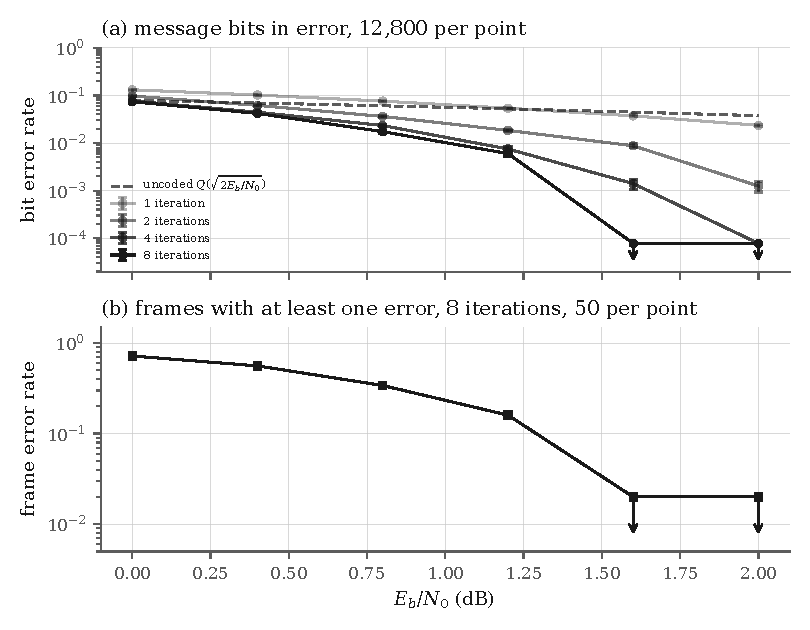
\includegraphics[width=\linewidth]{figures/turbo_waterfall}
  \caption{\turboWaterfallCaption}
  \label{fig:turbo-waterfall}
\end{figure}

\subsection{Extensions, and what is not attempted}
\label{sec:turbo:extensions}
\paragraph{What it would take to go further.}
The section's own statement is that no exact algorithm reaches the pair at the
lengths it is used at, and the referee past $K \le 17$ is a bound from one
side. What would give the pair an ensemble statement is the analogue of
Appendix~\ref{app:density-evolution}: track how the extrinsic information one
constituent decoder produces depends on what it is given, and read the
iteration's convergence off the pair of such curves --- the same fixed-point
reasoning as the erasure threshold, applied to two decoders in series rather
than to one graph. That would turn the measured waterfall into a predicted
one. Two code-side directions follow from Section~\ref{sec:turbo:discussion}'s
observation that the cycles, not the length, are what cost the iteration: an
interleaver designed to avoid short cycles rather than drawn at random, and
puncturing, which raises the rate and is what the transmitted word of
Equation~\ref{eq:turbo-word} deliberately does not do.

\paragraph{What is deliberately not attempted.}
Monotonicity in the iteration count, which is not an open question here but a
refused claim --- the measurement contradicts it and the section states the
weaker pair the sample supports. A blockwise decoding of the \emph{pair}: the
maximum over messages is well defined and no algorithm reaches it, so what is
carried is the constituent code's blockwise answer and the pair's bitwise one.
And non-binary constituent codes, for the reason
Section~\ref{sec:ldpc:extensions} gives: the channel and the ratio convention
are binary throughout, and every referee here is stated in those terms.

\section{The Properties That Referee Each Method}
\label{sec:properties}

An algorithm is accepted here against a property that is true independently of
this implementation. The properties are not interchangeable, and which one
applies is a statement about the method rather than a matter of convenience.
Each \emph{What pins it} paragraph above names one of the five kinds below,
and the regression suite marks every check with the kind it is: an oracle, a
simulated truth, a mathematical invariant, an edge case, or a structural
property of the code. A check that fits none of them is either a missing
category or a test with nothing to assert.

\subsection{Exact answers, where an oracle exists}
Where a quantity can be computed a second way that shares no recursion with the
first, equality is asserted to a stated tolerance. Direct marginalization over
$k^{n-2}$ internal assignments referees pruning; a sum over $k^T$ paths
referees the forward recursion; exhaustive enumeration over $q^{|V|}$
configurations referees a Potts marginal; enumeration of $(2n-5)!!$ topologies
referees a search. Every one is exponential, and that is what makes it an
oracle rather than a second opinion. \textbf{Two implementations agreeing prove
nothing if both are wrong}, so an accelerated method is pinned against the
reference and never against another acceleration.

\subsection{Structural invariants, where no oracle reaches}
Past the sizes enumeration allows, what remains are properties the model must
satisfy whatever the answer is:
\begin{itemize}
  \item rows of a transition matrix sum to one, and $\Pmat(0) = \mathbf{I}$;
  \item a reversible model satisfies detailed balance, $\pi_i \Q_{ij} = \pi_j \Q_{ji}$;
  \item the \emph{pulley principle}: on a reversible model the likelihood is
        invariant to where the root is placed along a branch, so a rooted
        computation and its re-rooting must agree exactly;
  \item a gradient matches central differences, relative to the gradient's own
        norm---entrywise fails wherever an entry is zero, and an absolute bound
        does not transfer across data sizes;
  \item an expectation-maximization iterate increases the likelihood
        monotonically.
\end{itemize}
None of these establishes that a method is right. Each establishes that a
specific way of being wrong did not happen, which is a weaker and more
defensible claim.

\subsection{Recovery, which is the acceptance test for a fit}
A likelihood that increases proves the optimizer runs, not that the model is
right. The acceptance test is to fit data simulated from known parameters and
require the intervals to cover the truth at their nominal rate over
independent replicates. Two qualifications are load-bearing. Where a model has
an exact symmetry---permuting the hidden states of an HMM or the components of
a mixture leaves the likelihood unchanged---recovery is stated \emph{up to that
symmetry}, and the alignment is part of the test. And coverage is measured as a
function of how identifiable the instance is, because a fixture chosen where
everything is well separated is a test of the fixture.

\subsection{Where the likelihood has no maximum, or no curvature}
Two failures are properties of models rather than defects, and both must be
handled before they are discovered.

An \emph{unbounded} likelihood has no maximum to find: put a Gaussian
component's mean on a single observation and let its variance go to zero and
the density there diverges. A fit that converges there was stopped by its
starting point or by a floor, and which one must be knowable---so the bound is
explicit, derived from the data rather than chosen, and reaching it is a
refusal rather than a clamp.

A \emph{flat} likelihood has a maximum that runs to the boundary: an
overdispersed count model approaches its Poisson limit as the dispersion grows,
and past the point where the overdispersion is smaller than the sampling noise
on measuring it, the data cannot tell one value from another. The two failures
are mirror images, and they announce themselves differently---the first as a
divergence, the second as a singular information matrix---which is why each is
measured rather than inferred from the other.

\subsection{Agreement across implementations is a tolerance}
\label{sec:tolerance}
An accelerated implementation is pinned against the reference within a
declared \emph{relative} tolerance, never bitwise. Relative, because a
log-likelihood is a sum over sites and an absolute bound fixed at one size does
not transfer to another. Keyed on the \emph{lowest} precision in the
comparison, because a single-precision device cannot be held to a
double-precision bound, and one bound loose enough for single precision would
let a broken double-precision backend pass. A discrepancy inside the tolerance
is not a defect and is not corrected; one outside it is not a tolerance to
loosen. The values themselves live beside the measurements they are derived
from, not here.

\subsection{Published constants, and asymptotic results}
Some claims come from outside entirely: the $(2n-5)!!$ count, Goemans--Williamson's
$0.87856$ for maximum cut, alpha expansion's factor of two, the
$8(\ln k + 2)$ bound on $k$-means$++$ seeding. These referee an implementation
at any size. \textbf{No asymptotic result is testable at the sizes an exact
oracle allows}, however: a threshold or a limit holds as the problem grows and
says nothing where enumeration can check it. Such a result is reported for
orientation and the per-instance property is what is asserted.

\section{Relevance to the Roadmap}
\label{sec:roadmap}

The problem classes are not applications. They are chosen so that
each abstraction is tested against something that is not the model it was
extracted from: a likelihood engine justified only by trees would be a
phylogenetics library, and an optimizer justified only by an HMM would
encode a chain.

The order the milestones take follows the dependency between the properties
above. Simulation and its ground truth come first, because every later claim is
checked against data whose generating parameters are known. The exact
evaluators come next, because they are the oracles the accelerated ones are
pinned to. Continuous optimization follows, since recovery is the acceptance
test and needs both. Discrete search and learned proposals come last, because
their acceptance criterion---reaching the optimum enumeration identifies---only
exists once enumeration does.

\subsection{Beyond the Roadmap}
\label{sec:bluesky}
Each problem statement above ends with what it would take to go further and
what it deliberately does not attempt. Three directions recur across them, and
they are worth stating once as a whole rather than eleven times in pieces.

\emph{A bound where there is no oracle.} The recurring gap is not speed: it is
that past a size, a search returns an answer nothing can score. Every section
that names a missing referee names the same kind of object --- a branch and
bound over topologies, a boundary contraction for a lattice, a density
evolution past the erasure channel, an enumerated maximum-posterior labelling
on one coupled instance. Each converts a reported optimum into a bracket, and
a bracket is the difference between a result and a measurement.

\emph{Learning as a proposal, never as an answer.} A learned policy, a learned
surrogate, a learned ground state and a learned decoder all enter this
document in the same position: they choose what to evaluate, and the thing
evaluated is still the objective the section defines. That is what keeps them
refereeable --- a proposal that fails is slower, where an answer that fails is
wrong --- and it is the reading the field's own reviews take of the
combinatorial case \citep{bengio2021, mazyavkina2021}. The architectures the
proposals would use are settled elsewhere and are cited rather than restated:
a graph network over the structure \citep{khalil2017}, an attention model over
its parts \citep{kool2019}. The standing caution is the one
Section~\ref{sec:potts:extensions} records --- such a method is measured
against a competently tuned classical baseline at a matched budget, or it has
not been measured \citep{angelini2023} --- and the standing requirement is
that a rate is reported with the interval, the seeds and the budget behind it
\citep{henderson2018, agarwal2021}.

\emph{Structure that is differentiable.} Section~\ref{sec:relaxation} and
Section~\ref{sec:tropical} approach one question from two sides: whether a
discrete structure can be moved by a gradient without becoming a different
problem. Both answer it the same way --- the relaxation must agree with what
it relaxes at every corner --- and both are limited by the same thing, which
is that the corner check needs an enumeration. Extending it to a space no
enumeration reaches is where the structured relaxations \citep{paulus2020} and
the parameterized topology spaces \citep{zhang2019} would have to meet.


\bibliographystyle{plainnat}
\bibliography{references}

\appendix

\section{Derivations Cited From the Text}
\label{app:derivations}

Each of these is standard; each is here because a claim in the main text
depends on it, and the main text cites rather than derives, for the reader
the preface names.

\subsection{Pruning is the marginalization over internal states}
\label{app:pruning}
Root $\tree$ at $\rootnode$ and write $z_u$ for the state at node $u$, so the
leaves' states at one site are the data $\data_s$ and the internal states are
summed. Along each branch the state evolves by the Markov process of
Section~\ref{sec:phylo}, and the branches are conditionally independent given
the state at their common node, so the joint over every node is
$p(z) = \pi_{z_{\rootnode}} \prod_{v \neq \rootnode}
\Pmat_{z_{\mathrm{pa}(v)} z_v}(t_v)$, and the site likelihood is its sum over
the internal states with the leaves clamped---the summand of
Equation~\ref{eq:site-independence}, with $k^{n-2}$ terms. Define
$L_u(i) = p(\data_s^{(u)} \mid z_u = i)$, the probability of the data at the
leaves below $u$ given $u$'s state. The subtrees hanging from $u$'s children
share no variable and, given $z_u$, no factor, so the sum over their states
factorizes into one sum per child:
\begin{equation*}
  L_u(i) = \prod_{v \in \mathrm{children}(u)} p(\data_s^{(v)} \mid z_u = i)
         = \prod_{v \in \mathrm{children}(u)} \sum_{j \in \states}
           \Pmat_{ij}(t_v)\, p(\data_s^{(v)} \mid z_v = j),
\end{equation*}
the second equality conditioning on $z_v$ and using that the data below $v$
depends on $z_u$ only through $z_v$. The inner probability is $L_v(j)$, which
is Equation~\ref{eq:pruning}; at a leaf $L_u(i) = \mathbb{1}[z_u = i]$
because the state is observed; and summing the root state against its prior
gives Equation~\ref{eq:root}. Nothing in the argument fixes the order of the
children or the depth of the tree, so the recursion is a post-order traversal
in which each node's sum is done once per parent state: $O(n k^2)$ per site
against $k^{n-2}$ terms. Each $L_u$ is linear in each $L_v$, so rescaling
$L_u$ by a positive $c_u$ scales the site likelihood by $\prod_u c_u$ and
nothing else, which is why the logarithm of the scaling may be accumulated
apart from the recursion and the rescaled recursion is a transformation of
this one rather than a second algorithm
\citep{felsenstein1981, felsenstein2004}.

\subsection{Forward--backward is the same marginalization on a chain}
\label{app:forward-backward}
With the factors of Section~\ref{sec:hmm} the joint over the hidden path and
the observations is $p(\hidden, \data) = \pi_{z_1}\,\emission_{z_1}(y_1)
\prod_{t > 1} \mathbf{A}_{z_{t-1} z_t}\, \emission_{z_t}(y_t)$, and the
evidence sums it over $k^T$ paths. Define $\alpha_t(i) = p(y_1, \dots, y_t,
z_t = i)$. Conditioning on $z_{t-1}$, and using that $y_1, \dots, y_{t-1}$
depend on $z_t$ only through $z_{t-1}$, splits the sum over the first $t - 1$
states from the rest:
$\alpha_t(i) = \big[\sum_j \alpha_{t-1}(j)\,\mathbf{A}_{ji}\big]\,
\emission_i(y_t)$, with $\alpha_1(i) = \pi_i\,\emission_i(y_1)$, and the
evidence is $\sum_i \alpha_T(i)$: Equation~\ref{eq:forward}. Define
$\beta_t(i) = p(y_{t+1}, \dots, y_T \mid z_t = i)$, so $\beta_T = 1$;
conditioning on $z_{t+1}$ in the same way gives the backward recursion of
Equation~\ref{eq:posterior}. The two meet at any position:
$p(z_t = i, \data) = \alpha_t(i)\,\beta_t(i)$, because the observations
before $t$ and after $t$ are independent given $z_t$, and dividing by the
evidence gives the posterior of Equation~\ref{eq:posterior}; the same split
one step wider gives the pairwise posterior
$p(z_{t-1} = i, z_t = j \mid \data) = \alpha_{t-1}(i)\,\mathbf{A}_{ij}\,
\emission_j(y_t)\,\beta_t(j) / p(\data)$, the sufficient statistic of the
expectation step.

The chain is the caterpillar tree of Section~\ref{sec:hmm} rooted at $z_1$:
each $z_t$ has one child $z_{t+1}$ carrying the branch factor $\mathbf{A}$ and
one observed leaf $y_t$ carrying the emission. Appendix~\ref{app:pruning}
then gives $L_{z_t}(i) = \emission_i(y_t)\,\sum_j \mathbf{A}_{ij}\,
L_{z_{t+1}}(j)$, so $L_{z_t}(i) = \emission_i(y_t)\,\beta_t(i)$ and
Equation~\ref{eq:root} is $\sum_i \pi_i\,\emission_i(y_1)\,\beta_1(i) =
\sum_i \alpha_1(i)\,\beta_1(i) = p(\data)$: pruning on the chain is the
backward pass, and the forward pass is the same recursion run toward the
other end with the prior entering as a leaf factor at $z_1$. Both passes in
the logarithm are the rescaled recursion of Appendix~\ref{app:pruning} with
the scale taken at every step. Replacing each sum by a maximum leaves every
step of the argument intact, since a maximum distributes over a product of
non-negative factors as a sum does, and gives Equation~\ref{eq:viterbi}
\citep{durbin1998, koller2009}.

\subsection{Sum-product on a tree, and its loopy stationary point}
\label{app:sum-product}
Both derivations above are one fact about a tree-structured factor graph.
Take an edge between factor $a$ and variable $i$ and remove it; because the
graph is a tree, the component containing $a$ is a subtree $\tree_{a \to i}$
that meets the rest only at $x_i$. Define the message from $a$ to $i$ as the
partition function of that subtree with $x_i$ clamped,
$m_{a \to i}(x_i) = \sum_{x_{\tree_{a \to i}} \setminus x_i}
\prod_{b \in \tree_{a \to i}} \psi_b(x_{\partial b})$, and $m_{i \to a}$
likewise for the subtree on $i$'s side. The subtrees hanging from $a$'s other
variables $j \in \partial a \setminus i$ are disjoint, so the sum over their
variables factorizes into a product of their partition functions, each a
function of its own $x_j$; and the subtrees hanging from $i$'s other factors
share only $x_i$, so their product is $m_{i \to a}(x_i)$. That is
Equation~\ref{eq:sum-product}, with the messages at a leaf variable or leaf
factor being $1$ and the factor itself. At any variable the whole graph is
the union of the subtrees on its factors, so $Z = \sum_{x_i} \prod_{a \in
\partial i} m_{a \to i}(x_i)$ and the marginal is that product normalized;
at a factor, $p(x_{\partial a}) \propto \psi_a(x_{\partial a}) \prod_{i \in
\partial a} m_{i \to a}(x_i)$. A message depends only on messages from
further from any chosen root, so one leaf-to-root pass computes every message
toward it and one root-to-leaf pass every message away, and every marginal
follows: two passes, each factor summed once per direction
\citep{pearl1988, kschischang2001, koller2009}. Pruning is this with a node's
state as the variable, a branch matrix as the factor between parent and
child, the prior as a factor on the root and a leaf's observation as an
indicator factor: $L_u(i)$ is the product of the factor-to-variable messages
from below, which is the variable-to-factor message $m_{u \to \psi_u}$ that
$u$ sends up its own branch. Forward--backward is this on the chain. The
argument used only that sum distributes over product, so max-product follows
by replacing every sum with a maximum, exact on a tree when the maximum is
unique.

On a graph with a cycle no edge separates the graph into two subtrees, so
the message has no such definition; iterating Equation~\ref{eq:sum-product}
regardless defines a map on messages, and a fixed point of that map is a
stationary point of the Bethe free energy, which Appendix~\ref{app:bethe}
derives for the pairwise case of Equation~\ref{eq:bethe} and which reads, for
factors of any degree,
\begin{equation}
  F_{\mathrm{Bethe}}
    = \sum_a \sum_{x_{\partial a}} b_a\,\big(\log b_a - \log \psi_a\big)
    - \sum_i (d_i - 1) \sum_{x_i} b_i \log b_i,
  \label{eq:bethe-factor}
\end{equation}
with $d_i$ the number of factors on $i$. On a tree $p(x) = \prod_a b_a /
\prod_i b_i^{\,d_i - 1}$ exactly, the beliefs being the true marginals, so
Equation~\ref{eq:bethe-factor} is $-\log Z$ and the stationary point is the
answer of the two passes; on a loopy graph the factorization fails and the
fixed point is the approximation
\citep{yedidia2005, mezard2009}.

\subsection{The Bethe free energy is stationary at a sum-product fixed point}
\label{app:bethe}
Write the beliefs of a pairwise graph as $b_i$ and $b_{ij}$ and constrain them
to be normalized and locally consistent, $\sum_{\sigma_j} b_{ij} = b_i$.
Introducing a multiplier $\lambda_{ij}(\sigma_i)$ for each consistency
constraint and setting the derivative of Equation~\ref{eq:bethe} to zero gives
$b_{ij} \propto \psi_{ij}\, e^{\lambda_{ij}(\sigma_i) + \lambda_{ji}(\sigma_j)}$
and $b_i \propto \psi_i\, e^{\sum_{j \in \partial i} \lambda_{ji}(\sigma_i) / (d_i - 1)}$;
identifying $e^{\lambda_{ji}(\sigma_i)}$ with $\prod_{l \in \partial i
\setminus j} m_{l \to i}(\sigma_i)$ turns the consistency constraint into
Equation~\ref{eq:bp-message}. So a fixed point of belief propagation is a
stationary point of the Bethe free energy and conversely; on a tree the Bethe
free energy is the exact variational free energy, which is why the fixed point
there gives $-\log Z$ \citep{yedidia2005}. The argument uses only that
each $b_a$ is a function of the variables its factor touches, so it holds
for factors of any degree, with Equation~\ref{eq:bethe-factor} in place of
Equation~\ref{eq:bethe} and $d_i - 1$ counting the factors on $i$ beyond
the first (Appendix~\ref{app:sum-product}).

\subsection{Detailed balance for a cluster move in a field}
\label{app:detailed-balance}
In the Edwards--Sokal representation the joint over spins and bonds is
$p(\sigma, \omega) \propto \prod_{\langle i,j \rangle : \omega_{ij} = 1}
(1 - e^{-\beta J_{ij}})\,\delta(\sigma_i, \sigma_j) \prod_{\omega_{ij} = 0}
e^{-\beta J_{ij}}\ \prod_i e^{\beta h_i(\sigma_i)}$, whose spin marginal is the
Boltzmann distribution of Equation~\ref{eq:potts}. Drawing bonds given spins
and then recolouring a bond cluster $\mathcal{C}$ uniformly are both Gibbs
steps at zero field, so the move preserves $p$ there. With a field the
recolouring is no longer a Gibbs step: the ratio of the target before and after
recolouring $\mathcal{C}$ from $\mu$ to $\nu$ is $\exp(\beta \sum_{i \in
\mathcal{C}} [h_i(\nu) - h_i(\mu)])$, the bond configuration being unchanged,
and a uniform proposal accepted with the Metropolis probability of
Equation~\ref{eq:cluster-accept} satisfies detailed balance with respect to
that ratio. Omitting the accept step gives a chain that runs and mixes and
converges to the zero-field distribution, which is why the distributional
test is run with a field as well as without.

\subsection{The exchange ratio in parallel tempering}
\label{app:exchange}
The replicas' joint target is the product $\prod_r \exp(-\beta_r E(\sigma_r))$.
Swapping the configurations of replicas $i$ and $j$ changes it by
$\exp(-\beta_i E_j - \beta_j E_i) / \exp(-\beta_i E_i - \beta_j E_j)
= \exp[(\beta_i - \beta_j)(E_i - E_j)]$, and the proposal is symmetric, so the
Metropolis acceptance is Equation~\ref{eq:exchange}. Each replica's marginal
under the joint is its own tempered Boltzmann distribution whatever the
exchanges do, which is the property the per-replica goodness-of-fit test
asserts.

\subsection{Density evolution on the erasure channel}
\label{app:density-evolution}
On a cycle-free $(d_v, d_c)$ graph the messages arriving at a node are
independent, so the erasure probability of a message is a number rather than
a distribution and Equation~\ref{eq:tanh-rule} reduces to a scalar
recursion. A check-to-bit message is known only if every other incoming
bit message is known; a bit-to-check message is erased only if the channel
and every other incoming check message are. With $x_\ell$ the probability
that a bit-to-check message is erased after $\ell$ iterations,
\begin{equation}
  x_0 = \epsilon,
  \qquad
  x_\ell = \epsilon \big( 1 - (1 - x_{\ell-1})^{d_c - 1} \big)^{d_v - 1},
  \label{eq:density-evolution}
\end{equation}
the recursion \citet[Sec.~3.12]{richardson2008} derives and names density
evolution. The right-hand side is increasing in $x_{\ell-1}$ and in
$\epsilon$, so $x_\ell$ is non-increasing and its limit is the largest fixed
point in $[0, \epsilon]$; the threshold $\epsilon^\star$ is the largest
$\epsilon$ for which that fixed point is zero, found by bisection, and for
$(3,6)$ it is $0.4294$, with $0.3834$ for $(4,8)$ and $0.5176$ for
$(3,5)$. A finite code is not cycle-free, but the neighbourhood of a bit to
depth $\ell$ is a tree with probability tending to one as $n$ grows at
fixed $\ell$, which is why the recursion is the limit of the flooding
decoder and why the code at size is held to bracketing $\epsilon^\star$
rather than to a per-draw agreement---the rule this repository states for
every asymptotic result (Section~\ref{sec:properties}).

\subsection{The delta method for an interval at a fit}
\label{app:delta}
At a maximum $\hat\params$ of the log-likelihood, the observed information
$\mathcal{I} = -\nabla^2 \log p(\data \mid \hat\params)$ gives the asymptotic
covariance $\Sigma = \mathcal{I}^{-1}$ of $\hat\params$. A constrained
parameter $\constrained(\params)$ is a smooth function of $\params$, so to first
order $\mathrm{Var}(\constrained(\hat\params)) \approx J \Sigma J^{\top}$ with
$J = \partial \constrained / \partial \params$ at $\hat\params$. The statement
is asymptotic in the sample size and requires $\mathcal{I}$ to be invertible;
a singular or ill-conditioned information is a parameter the data does not
identify, and the interval is refused rather than reported
(Section~\ref{sec:properties}).

\section{Derivations for the Actor--Critic}
\label{app:rl}

\paragraph{Any state-dependent baseline leaves the estimator unbiased.}
For a function $b$ of the state alone,
$\mathbb{E}_{a \sim \pi(\cdot \mid s)}[\nabla \log \pi(a \mid s)\, b(s)]
= b(s) \sum_a \nabla \pi(a \mid s) = b(s)\, \nabla \sum_a \pi(a \mid s) = 0$,
so subtracting $b(s_t)$ from $G_t$ in \eqref{eq:reinforce} changes no
expectation. The variance of the per-step term $\nabla \log \pi \cdot (G_t - b)$
is minimized over constant $b$ by a weighted mean of $G_t$, and over
state-dependent $b$ the value $V^\pi(s_t)$ is the choice that removes the part
of $G_t$ predictable from the state; a fitted critic approximates it, and its
error costs variance, never bias, as long as the fit does not read the action
sampled at that step \citep{suttonbarto2018}.

\paragraph{The generalized advantage telescopes to its two limits.}
With $\delta_t = R_t + V(s_{t+1}) - V(s_t)$ and $V(s_T) = 0$,
$\sum_{l=0}^{T-t-1} \delta_{t+l} = \sum_{u \ge t} R_u - V(s_t) = G_t - V(s_t)$,
which is \eqref{eq:gae} at $\lambda = 1$; at $\lambda = 0$ only $\delta_t$
survives. The exponential weights interpolate the two, and the bias of
$A_t^{(\lambda)}$ as an estimate of the true advantage is
$O(\lambda^{k})$ in the critic's error at $k$ steps ahead
\citep{schulman2016}.

\paragraph{PUCT as policy improvement.}
With exact leaf values and one decision of depth, every backed-up value in
\eqref{eq:puct} is $Q^*(s, a)$ exactly, and as $N(s) \to \infty$ the bonus
of every action vanishes relative to the gap between the best mean and the
rest, so the most visited action is an argmax of $Q^*$. At depth the means
are of returns under the search's own descents, which concentrate on the
children it rates highest; the normalized visit counts are then a
distribution whose one-step expected value under $Q^\pi$ is at least the
prior's, which is the policy-improvement step of policy iteration with the
prior as $\pi$ and the visit distribution as the improved policy
\citep{suttonbarto2018, silver2017}. The regression suite checks both on
the Potts chain: the argmax exactly at depth one, and the improvement on 13
of 14 sampled states at depth three, the exception being a state whose prior
already puts most of its mass on an optimal move.

\paragraph{The clipped objective at the collecting policy.}
With $\pi = \pi_{\mathrm{old}}$, $\rho_t = 1$ for every decision, so both
arguments of the minimum in \eqref{eq:ppo-clip} equal $A_t$ and
$\nabla \rho_t = \nabla \log \pi(a_t \mid s_t)$; the gradient of
\eqref{eq:ppo-clip} is $\sum_t \nabla \log \pi(a_t \mid s_t)\, A_t$, the
actor--critic's estimator. Away from the collecting policy the minimum
removes the gradient wherever the ratio has left $[1-\epsilon, 1+\epsilon]$
in the direction the advantage would push it, which is the pessimistic
bound on the surrogate improvement that licenses the reuse of a batch
\citep{schulman2017}.

\section{Derivations of the Bounds}
\label{app:bounds}

\paragraph{The plug-in bound, \eqref{eq:plugin-bound}.}
$\ell^\ast(\tree)$ is a maximum over the feasible set $\branch \ge 0$, and
$\hat{\branch}$ lies in it by construction: projected gradient descent on the
convex least-squares objective clamps every iterate to the non-negative
orthant, so the value at $\hat{\branch}$ is one of the values maximized over.
Equality holds exactly when $\hat{\branch}$ is a maximizer.

\paragraph{The parsimony bound, \eqref{eq:parsimony-bound}.}
Write $a_e = e^{-k t_e/(k-1)} \in [0,1]$. Each entry of $\Pmat(t_e)$ is affine
in $a_e$ and each branch appears exactly once in the product of
\eqref{eq:pruning}, so the site likelihood is a polynomial of degree at most
one in each $a_e$: multilinear. A multilinear function on a box attains its
maximum at a vertex, where each $\Pmat_e$ is either $\mathbf{I}$ (no change
permitted) or $\mathbf{J}/k$ (the child's state independent of the parent's,
at weight $1/k$). Root the tree at leaf $1$, which the pulley principle
permits for a reversible model. At a vertex with cut set $C$ (the branches
carrying $\mathbf{J}/k$), the site likelihood is a sum over ancestral
assignments constant on each component of $\tree \setminus C$:
$\pi(x_{1,s})\,k^{-|C|}\,k^{\,\ell'}$, with $\ell'$ the number of
components containing no leaf (each contributes a free sum over $k$ states),
provided every leafy component is monochromatic, and zero otherwise.
Merging each leafless component into a neighbour across one of its boundary
branches removes one cut and one leafless component at a time and leaves a
valid partition with $|C| - \ell'$ cuts, all of whose components are leafy
and monochromatic; assigning each its leaf state gives an ancestral labelling
with at most $|C| - \ell'$ changes, so $F_s \le |C| - \ell'$ by minimality of
the Fitch score. Hence every vertex value is at most
$\pi(x_{1,s})\,k^{-F_s}$, and so is the maximum over the box. Summing over
sites gives \eqref{eq:parsimony-bound}; the regression suite enumerates the
$2^{|E|}$ vertices at five taxa and finds the bound attained on every site.
The entrywise limit $\sup_t \Pmat_{ij}(t)$, one on the diagonal and $1/k$
off it, gives a bound this one dominates, because that matrix is not
row-stochastic and the polynomial is increasing in every entry.

\paragraph{The block-frequency bracket, \eqref{eq:block-frequency-bound}.}
Two claims, and only the second needs an argument. First, the partition is a
partition: every site lies in exactly one block, the frequent blocks
contribute $\ell_{\mathcal{F}}$ by Equation~\ref{eq:site-patterns}, and each
of the remaining $B$ sites contributes a term lying in
$[\underline\lambda, \overline\lambda]$ by definition, so summing gives
\eqref{eq:block-frequency-bound}. Second, $\underline\lambda$ and
$\overline\lambda$ are computable in one pass. Run \eqref{eq:pruning} in the
log domain and carry an interval $[\underline{L}_u(i), \overline{L}_u(i)]$ in
place of each partial. A leaf $v$ observed in state $x$ sends its parent the
column $\Pmat_{\cdot x}(t_v)$, so over every $x$ that message lies entrywise
in $[\min_j \Pmat_{ij}(t_v), \max_j \Pmat_{ij}(t_v)]$, which is the leaf case
and the only place the data enters. Above a leaf, $\sum_j \Pmat_{ij}(t_v)
L_v(j)$ and the product over children in \eqref{eq:pruning} are non-decreasing
in each $L_v(j)$, since transition probabilities and partials are
non-negative, and so is the root sum \eqref{eq:root}; a non-decreasing
function of arguments confined to intervals is confined to the interval its
endpoints give, so the bounds propagate and $\underline\lambda$,
$\overline\lambda$ bracket $\log p(x \mid \tree, \branch, \Q)$ for every
$x \in \states^n$ at once. The relaxation is that each child's extreme is
taken independently of the others: the bracket is therefore sound, and no
single column need attain either end. $\underline\lambda = -\infty$ where a
branch of length zero makes some column impossible, which is that column's
value and not a failure. The regression suite enumerates all $k^{\,n} = 256$
columns of the four-taxon fixture and finds none outside the bracket.

\paragraph{The mean-field bound, \eqref{eq:mean-field-bound}.}
For any distribution $q$ on configurations,
$\log Z = \mathbb{E}_q[-\energy] + H(q) + \mathrm{KL}(q \,\|\, p)$, and the
divergence is non-negative (Gibbs' inequality). Restricting $q$ to products
and evaluating the expectation gives the right-hand side; the fixed-point
iteration $q_i \propto \exp(h_i + \sum_{j \in \partial i} J_{ij} q_j)$
ascends it coordinate-wise, and the bound holds at every iterate, so a
truncated iteration is a looser bound and never a wrong one
\citep{mackay2003, mezard2009}.

\paragraph{The spanning-tree bound, \eqref{eq:spanning-tree-bound}.}
$\log Z(\theta)$ is the log-normalizer of an exponential family and therefore
convex in $\theta$. For trees $T$ with weights $\rho(T)$ and parameters
$\theta(T)$ with $\sum_T \rho(T)\theta(T) = \theta$, Jensen gives
$\log Z(\theta) \le \sum_T \rho(T) \log Z(\theta(T))$. The implementation
takes one tree per edge, built by breadth-first search from that edge so it
contains it, weighted uniformly; an edge appearing in a fraction $\rho_e$ of
the trees carries $J_e/\rho_e$ on each tree containing it and $0$ elsewhere,
so the weighted mean is $J_e$, and the fields are shared. Each
$\log Z(\theta(T))$ is exact by the leaf-to-root recursion, in the log
domain. The bound is tight when the graph is a tree \citep{wainwright2005}.

\paragraph{The ground-state bracket, \eqref{eq:ground-state-bounds}.}
$Z(\beta) = \sum_\sigma e^{-\beta \energy(\sigma)}$ has $k^N$ terms, each at
most $e^{-\beta E_{\min}}$ and at least one equal to it, so
$-\beta E_{\min} \le \log Z(\beta) \le N \log k - \beta E_{\min}$. Combining
with $L \le \log Z(\beta) \le U$ and dividing by $\beta > 0$ gives the
bracket; as $\beta$ grows the $N \log k$ term is divided away, until the
bounds on $\log Z$ themselves loosen.

\section{Algorithms Cited From the Text}
\label{app:algorithms}

The algorithms each problem statement cites, grouped by what each is for:
initializers, which choose where a search starts; samplers, which draw from a
distribution at a temperature; optimizers, which move toward an optimum; and
surrogates, which stand in for an expensive evaluation. They are collected
here rather than at the point of use because most of them apply to more than
one problem, and a statement of an algorithm belongs where it can be cited
from each. Four algorithms stay in the body, because there the text derives
them as it states them: forward simulation, Algorithm~\ref{alg:simulate};
neighbor joining, Algorithm~\ref{alg:neighbor-joining}; the Wolff move in an
external field, Algorithm~\ref{alg:wolff-field}; and the data-sampled
burn-in, Algorithm~\ref{alg:graph-burnin}.

\subsection{Initializers}
\label{app:algorithms:initializers}

\begin{algorithm}[htbp]
\caption{$k$-means$++$ seeding of $K$ centres, Equation~\ref{eq:kmeanspp}}
\label{alg:kmeanspp}
\begin{algorithmic}[1]
\State draw $c_1$ uniformly from the observations $y_1, \dots, y_N$
\For{$j = 1$ to $K - 1$}
  \State $D(y) \gets \min_{j' \le j} |y - c_{j'}|$ for every observation $y$
  \State draw $c_{j+1} = y$ with probability $D(y)^2 / \sum_{y'} D(y')^2$
\EndFor
\State \Return the centres $c_1, \dots, c_K$
\end{algorithmic}
\end{algorithm}

\begin{algorithm}[htbp]
\caption{The closest tree of a Hadamard spectrum, Equation~\ref{eq:hadamard}}
\label{alg:hadamard-start}
\begin{algorithmic}[1]
\State recode the alignment to two states and index the $2^{n-1}$ patterns by
       the set of taxa differing from a reference taxon
\State $s \gets$ the observed pattern frequencies;
       $q \gets \hadamard^{-1} \log(\hadamard s)$
\State $\mathcal{S} \gets \varnothing$
\For{each split in decreasing order of its weight in $q$}
  \If{the split is compatible with every split in $\mathcal{S}$}
    \State $\mathcal{S} \gets \mathcal{S} \cup \{\text{split}\}$
  \EndIf
  \State \textbf{stop} once $|\mathcal{S}| = n - 3$
\EndFor
\State \Return the topology whose internal edges are $\mathcal{S}$, with the
       corresponding weights as branch lengths
\end{algorithmic}
\end{algorithm}

\begin{algorithm}[htbp]
\caption{Multi-start from a generator, at a declared budget}
\label{alg:random-restart}
\begin{algorithmic}[1]
\State $\params_0 \gets$ the objective's own start, or that start tilted by a
       fixed alternating amount where it is stationary
\For{$r = 1$ to $R$}
  \State $\params_r \gets \params_0 + \varepsilon_r$, $\varepsilon_r$ drawn
         from the passed-in generator
\EndFor
\State fit from every $\params_r$, each fit charged to the shared budget of
       objective evaluations
\State \Return every fit with its spread, and the best of them --- never the
       best alone
\end{algorithmic}
\end{algorithm}

\subsection{Samplers}
\label{app:algorithms:samplers}

\begin{algorithm}[htbp]
\caption{One heat-bath sweep at inverse temperature $\beta$,
Equation~\ref{eq:heat-bath}}
\label{alg:heat-bath}
\begin{algorithmic}[1]
\For{each node $i$ of $\graph$, in a fixed order}
  \State $p(\sigma) \propto \exp\!\big(\beta [\sum_{j \in \partial i} J_{ij}
         \delta(\sigma, \sigma_j) + h_i(\sigma)]\big)$ for
         $\sigma \in \{1, \dots, q\}$
  \State draw $\sigma_i \sim p$ \Comment{$\beta \to \infty$ is the argmax,
         which is iterated conditional modes}
\EndFor
\State \Return the configuration after every node has been updated once
\end{algorithmic}
\end{algorithm}

\begin{algorithm}[htbp]
\caption{A cluster move at zero field, Edwards--Sokal bonds}
\label{alg:cluster-move}
\begin{algorithmic}[1]
\State refuse the move if any $J_{ij} < 0$, where $1 - e^{-\beta J_{ij}}$ is
       not a probability
\For{each edge $\langle i,j \rangle$ with $\sigma_i = \sigma_j$}
  \State place a bond with probability $1 - e^{-\beta J_{ij}}$
\EndFor
\State $\mathcal{C} \gets$ the bond-connected components; in Wolff, the one
       component containing a uniformly drawn root
\For{each component in $\mathcal{C}$}
  \State draw a new label $\nu$ uniformly from $\{1, \dots, q\}$
  \State recolour the component to $\nu$, accepted with
         Equation~\ref{eq:cluster-accept} where a field is present
\EndFor
\end{algorithmic}
\end{algorithm}

\begin{algorithm}[htbp]
\caption{Parallel tempering over $R$ replicas, Equation~\ref{eq:exchange}}
\label{alg:parallel-tempering}
\begin{algorithmic}[1]
\State $T_1 < \dots < T_R$; replica $r$ draws from its own generator, spawned
       from one parent that draws only the exchange uniforms
\For{each sweep of the budget}
  \For{$r = 1$ to $R$}
    \State advance replica $r$ by one sweep at $\beta_r = 1/T_r$
           \Comment{Algorithm~\ref{alg:heat-bath} or~\ref{alg:cluster-move}}
  \EndFor
  \For{each adjacent pair $(r, r+1)$}
    \State exchange the configurations with probability
           $\min\{1, \exp[(\beta_r - \beta_{r+1})(E_r - E_{r+1})]\}$
  \EndFor
  \State record the cold replica's state, and the acceptance of every pair
\EndFor
\State \Return the lowest energy seen, and the cold replica's recorded
       weights, Equation~\ref{eq:tempered-weight}
\end{algorithmic}
\end{algorithm}

\begin{algorithm}[htbp]
\caption{One block sweep over a chain, given the rest of the model}
\label{alg:chain-block}
\begin{algorithmic}[1]
\State run the forward recursion Equation~\ref{eq:forward} over the chain,
       keeping every $\alpha_t$
\State draw $z_T \sim \alpha_T$, normalized
\For{$t = T - 1$ down to $1$}
  \State draw $z_t$ with probability
         $\propto \alpha_t(z_t)\, \mathbf{A}_{z_t z_{t+1}}$
\EndFor
\State \Return the path, one exact draw from its conditional and not a
       sequence of single-site updates
\end{algorithmic}
\end{algorithm}

\subsection{Optimizers}
\label{app:algorithms:optimizers}

\begin{algorithm}[htbp]
\caption{Alpha expansion, Equation~\ref{eq:alpha-expansion}}
\label{alg:alpha-expansion}
\begin{algorithmic}[1]
\State $\sigma \gets$ any labelling
\Repeat
  \For{each label $\alpha \in \{1, \dots, q\}$}
    \State build the two-state graph in which every site keeps $\sigma_i$ or
           switches to $\alpha$
    \State $\sigma' \gets$ the labelling of its minimum $s$--$t$ cut
    \If{$\energy(\sigma') < \energy(\sigma)$} $\sigma \gets \sigma'$ \EndIf
  \EndFor
\Until{no expansion lowers the energy}
\State \Return $\sigma$ \Comment{within the constant of
       Equation~\ref{eq:alpha-expansion} of the optimum, provided each
       expansion was solved exactly}
\end{algorithmic}
\end{algorithm}

\begin{algorithm}[htbp]
\caption{Hill climbing over a structural neighbourhood}
\label{alg:hill-climbing}
\begin{algorithmic}[1]
\State $x \gets$ a start; $\mathrm{score}(x) \gets$ its full evaluation
\Repeat
  \State $\mathcal{N} \gets \neighbourhood(x)$, each candidate scored at most
         once and charged to the budget
  \State $x' \gets \arg\max_{y \in \mathcal{N}} \mathrm{score}(y)$
  \If{$\mathrm{score}(x') > \mathrm{score}(x)$} $x \gets x'$ \EndIf
\Until{no neighbour improves, or the budget is spent}
\State \Return $x$, its score always a full evaluation and never a surrogate's
\end{algorithmic}
\end{algorithm}

\begin{algorithm}[htbp]
\caption{Expectation--maximization on a chain, or without one}
\label{alg:baum-welch}
\begin{algorithmic}[1]
\Repeat
  \State \textbf{E step:} the posteriors of Equation~\ref{eq:posterior} by
         forward--backward; on a model with no chain, the responsibilities of
         Equation~\ref{eq:responsibilities} by a division
  \State \textbf{M step:} re-estimate $\bpi$ and $\mathbf{A}$ in closed form
         from the posterior counts, and the emission parameters by the
         family's own rule --- itself an optimization where no closed form
         exists
  \State assert the likelihood did not decrease
\Until{the increase falls below a tolerance, or the iteration cap is reached}
\end{algorithmic}
\end{algorithm}

\begin{algorithm}[htbp]
\caption{Sum-product decoding in the log domain,
Equation~\ref{eq:tanh-rule}}
\label{alg:sum-product-decode}
\begin{algorithmic}[1]
\State $m_{b \to i} \gets 0$ for every edge; $L_i$ from
       Equation~\ref{eq:ldpc-llr}
\For{iteration $1$ to the cap}
  \State $m_{i \to a} \gets \mathrm{clip}(L_i + \sum_{b \in \partial i
         \setminus a} m_{b \to i})$ for every edge, at once
  \State $m_{a \to i} \gets 2 \operatorname{artanh} \prod_{j \in \partial a
         \setminus i} \tanh (m_{j \to a}/2)$, or
         Equation~\ref{eq:min-sum} for min-sum
  \State $\tilde L_i \gets L_i + \sum_{b \in \partial i} m_{b \to i}$;
         $\hat c_i \gets \mathbb{1}[\tilde L_i < 0]$
  \State \textbf{stop} if every bit is decided and $\parity \hat c = 0$
\EndFor
\State \Return $\hat c$, and whether the syndrome check was reached --- a
       failure here is the event a block error rate counts
\end{algorithmic}
\end{algorithm}

\begin{algorithm}[htbp]
\caption{Turbo decoding: the serial extrinsic exchange,
Equation~\ref{eq:extrinsic}}
\label{alg:turbo-decode}
\begin{algorithmic}[1]
\State split the received ratios into $L^{s}, L^{p1}, L^{p2}$ and the second
       encoder's tail, Equation~\ref{eq:turbo-word}
\State $L^{a} \gets 0$ over the first chain's $K + m$ steps
\For{iteration $1$ to the cap}
  \State $\tilde L^{1} \gets$ BCJR$(L^{s}, L^{p1}, L^{a})$ by
         Equation~\ref{eq:bcjr}; $L^{e1} \gets \tilde L^{1} - L^{s} - L^{a}$
  \State $\tilde L^{2} \gets$ BCJR$(\Pi L^{s}, L^{p2}, \Pi L^{e1})$, the
         message positions interleaved and the tails left alone
  \State $L^{a} \gets \Pi^{-1}(\tilde L^{2} - \Pi L^{s} - \Pi L^{e1})$
  \State \textbf{stop} if the two chains' hard decisions on $u$ agree
\EndFor
\State \Return $\hat u_i = \mathbb{1}[(\Pi^{-1}\tilde L^{2})_i < 0]$, and
       whether the two agreed --- which is a stopping rule and not a
       certificate, since the graph has cycles
\end{algorithmic}
\end{algorithm}

\subsection{Surrogates}
\label{app:algorithms:surrogates}

\begin{algorithm}[htbp]
\caption{Ranking a neighbourhood by a surrogate, Section~\ref{sec:surrogates}}
\label{alg:surrogate-rank}
\begin{algorithmic}[1]
\State $\mathcal{N} \gets \neighbourhood(x)$
\State $\hat s(y) \gets$ the surrogate's value at every $y \in \mathcal{N}$,
       one cheap pass each
\If{the surrogate is an analytic bound}
  \State discard every $y$ whose bound cannot beat the incumbent
         \Comment{certified: no violation is permitted on any structure an
         oracle can score}
\Else
  \State shift $\hat s$ by a quantile of the held-out residuals, to the
         coverage the predictor claims
\EndIf
\State evaluate in full the best $\kappa$ candidates by $\hat s$, and the
       accepted move in full whatever its rank
\State \Return the accepted move, with a reported score that is always a full
       evaluation
\end{algorithmic}
\end{algorithm}

\begin{algorithm}[htbp]
\caption{The block-frequency bracket, Equation~\ref{eq:block-frequency-bound}}
\label{alg:block-frequency}
\begin{algorithmic}[1]
\State cut the $L$ columns into $\lfloor L/N \rfloor$ blocks of $N$ consecutive
       sites, and a shorter remainder if $N \nmid L$
       \Comment{a remainder is never equal to a full block}
\State count the occurrences of each distinct block;
       $\mathcal{F} \gets$ those occurring at least $m$ times
\State $\ell_{\mathcal{F}} \gets$ Equation~\ref{eq:site-patterns} over the
       columns of $\mathcal{F}$, each weighted by its block's count
       \Comment{a column shared by two frequent blocks is one pattern with the
       counts added}
\State $B \gets L - $ the sites $\mathcal{F}$ covers
\State $\underline\lambda, \overline\lambda \gets$
       Equation~\ref{eq:pruning} with each leaf's message replaced by the
       extremes of its transition row, one pass, no data read
\State \Return
       $[\ell_{\mathcal{F}} + B \underline\lambda,\;
         \ell_{\mathcal{F}} + B \overline\lambda]$, and
       $\ell_{\mathcal{F}} \cdot L / (L - B)$ as the point prediction that
       ranks
\end{algorithmic}
\end{algorithm}

\section{Reference Taxonomy}
\label{app:taxonomy}

Grouped as the repository groups them, so one routing table serves the code and
the documents alike. Within a group, books come first, then reviews, then the
papers an algorithm implements or a proposal needs as its oracle.

\paragraph{Infrastructure (build, structure, and speed).}
Software craft: \citet{martin2008}, \citet{blandy2021}, \citet{ramalho2022}.
Systems and hardware, including memory hierarchies and parallel kernels:
\citet{bryant2015}, \citet{pmpp2022}. Python performance:
\citet{gorelick2020}, \citet{antao2023}.

\paragraph{Optimization (discrete and continuous).}
Algorithms and discrete mathematics: \citet{clrs2022}, \citet{rosen2019},
\citet{papadimitriou1998}; the papers behind the cut-based solvers,
\citet{kolmogorov2004} on which energies a cut minimizes and
\citet{boykov2004} on the max-flow they run. Numerical optimization:
\citet{nocedal2006}, \citet{boyd2004} for the semidefinite certificate;
\citet{hansen2001} for the covariance-adapting evolution strategy proposed as
a population baseline. Probabilistic inference and message passing:
\citet{mackay2003}, \citet{koller2009}, \citet{frey1998}, \citet{ortega2022},
\citet{bishop2006}, \citet{murphy2023}; the review \citet{wainwright2008};
the papers \citet{wainwright2005} and \citet{wainwright2005map} for the
tree-reweighted bounds, \citet{hsu2012} for spectral initialization of a
hidden Markov model, and \citet{banerjee2005} for the divergence a seeding of
an exponential family draws under. Statistical physics and Monte Carlo: \citet{mezard2009},
\citet{newman1999}, \citet{krauth2006}, \citet{landau2014}; the reviews
\citet{betancourt2017} and \citet{schollwoeck2011}; the paper
\citet{machta2010} for population annealing. Information theory and
geometry: \citet{amari2016}, \citet{cover2006}. Learning and reinforcement
learning: \citet{goodfellow2016}, \citet{prince2023}, \citet{suttonbarto2018},
\citet{lapan2020}, \citet{raschka2024}; the papers \citet{sutton1999} and
\citet{bacon2017} for options, and \citet{schrittwieser2020} for planning
with a learned model. Learning for combinatorial optimization: the reviews
\citet{bengio2021} and \citet{mazyavkina2021}; the papers \citet{khalil2017},
\citet{kool2019}, \citet{paulus2020}, \citet{henderson2018},
\citet{agarwal2021}, and the pair \citet{schuetz2022} and
\citet{angelini2023}.

\paragraph{Application (the science).}
Phylogenetics: \citet{felsenstein2004}, \citet{durbin1998},
\citet{compeau2015}, \citet{pachter2005}, \citet{yang2014}; the papers
\citet{whidden2015}, \citet{azouri2021}, \citet{zhang2018}, \citet{zhang2019},
\citet{speyer2004}, \citet{altekar2004}, and the external baselines
\citet{minh2020} and \citet{kozlov2019}; distance and spectral methods:
\citet{saitou1987}, \citet{atteson1999}, \citet{steel1994},
\citet{hendy1993}, \citet{mossel2006}, with \citet{hsu2012} as the bridge.
Information and coding:
\citet{blahut2003}, \citet{richardson2008}, with \citet{nielsen2010} as
background only; the papers
\citet{gallager1962}, \citet{mackay2004} and \citet{nachmani2018}.

\end{document}
